%Version 3.1 December 2024
%DIF LATEXDIFF DIFFERENCE FILE
%DIF DEL old/main-file.tex   Tue Feb 10 13:18:58 2026
%DIF ADD new/main-file.tex   Tue Feb 10 12:54:31 2026
% See section 11 of the User Manual for version history
%
%%%%%%%%%%%%%%%%%%%%%%%%%%%%%%%%%%%%%%%%%%%%%%%%%%%%%%%%%%%%%%%%%%%%%%
%%                                                                 %%
%% Please do not use \input{...} to include other tex files.       %%
%% Submit your LaTeX manuscript as one .tex document.              %%
%%                                                                 %%
%% All additional figures and files should be attached             %%
%% separately and not embedded in the \TeX\ document itself.       %%
%%                                                                 %%
%%%%%%%%%%%%%%%%%%%%%%%%%%%%%%%%%%%%%%%%%%%%%%%%%%%%%%%%%%%%%%%%%%%%%

%%\documentclass[referee,sn-basic]{sn-jnl}% referee option is meant for double line spacing

%%=======================================================%%
%% to print line numbers in the margin use lineno option %%
%%=======================================================%%

%%\documentclass[lineno,pdflatex,sn-basic]{sn-jnl}% Basic Springer Nature Reference Style/Chemistry Reference Style

%%=========================================================================================%%
%% the documentclass is set to pdflatex as default. You can delete it if not appropriate.  %%
%%=========================================================================================%%

%%\documentclass[sn-basic]{sn-jnl}% Basic Springer Nature Reference Style/Chemistry Reference Style

%%Note: the following reference styles support Namedate and Numbered referencing. By default the style follows the most common style. To switch between the options you can add or remove “Numbered” in the optional parenthesis. 
%%The option is available for: sn-basic.bst, sn-chicago.bst%  
 
%%\documentclass[pdflatex,sn-nature]{sn-jnl}% Style for submissions to Nature Portfolio journals
%%\documentclass[pdflatex,sn-basic]{sn-jnl}% Basic Springer Nature Reference Style/Chemistry Reference Style
%DIF 33c33
%DIF < \documentclass[pdflatex,sn-mathphys-num]{sn-jnl}% Math and Physical Sciences Numbered Reference Style
%DIF -------
\documentclass[sn-mathphys-num]{sn-jnl}% Math and Physical Sciences Numbered Reference Style %DIF > 
%DIF -------
%%\documentclass[pdflatex,sn-mathphys-ay]{sn-jnl}% Math and Physical Sciences Author Year Reference Style
%%\documentclass[pdflatex,sn-aps]{sn-jnl}% American Physical Society (APS) Reference Style
%%\documentclass[pdflatex,sn-vancouver-num]{sn-jnl}% Vancouver Numbered Reference Style
%%\documentclass[pdflatex,sn-vancouver-ay]{sn-jnl}% Vancouver Author Year Reference Style
%%\documentclass[pdflatex,sn-apa]{sn-jnl}% APA Reference Style
%%\documentclass[pdflatex,sn-chicago]{sn-jnl}% Chicago-based Humanities Reference Style

%%%% Standard Packages
%%<additional latex packages if required can be included here>

\usepackage{graphicx}%
\usepackage{multirow}%
\usepackage{amsmath,amssymb,amsfonts}%
\usepackage{amsthm}%
\usepackage{mathrsfs}%
\usepackage[title]{appendix}%
\usepackage{xcolor}%
\usepackage{textcomp}%
\usepackage{manyfoot}%
\usepackage{booktabs}%
\usepackage{algorithm}%
\usepackage{algorithmicx}%
\usepackage{algpseudocode}%
\usepackage{listings}%

% \usepackage{cite}
\usepackage{balance}
\usepackage{booktabs}
\usepackage{subcaption}

%%%%

%%%%%=============================================================================%%%%
%%%%  Remarks: This template is provided to aid authors with the preparation
%%%%  of original research articles intended for submission to journals published 
%%%%  by Springer Nature. The guidance has been prepared in partnership with 
%%%%  production teams to conform to Springer Nature technical requirements. 
%%%%  Editorial and presentation requirements differ among journal portfolios and 
%%%%  research disciplines. You may find sections in this template are irrelevant 
%%%%  to your work and are empowered to omit any such section if allowed by the 
%%%%  journal you intend to submit to. The submission guidelines and policies 
%%%%  of the journal take precedence. A detailed User Manual is available in the 
%%%%  template package for technical guidance.
%%%%%=============================================================================%%%%

%% as per the requirement new theorem styles can be included as shown below
\theoremstyle{thmstyleone}%
\newtheorem{theorem}{Theorem}%  meant for continuous numbers
%%\newtheorem{theorem}{Theorem}[section]% meant for sectionwise numbers
%% optional argument [theorem] produces theorem numbering sequence instead of independent numbers for Proposition
\newtheorem{proposition}[theorem]{Proposition}% 
%%\newtheorem{proposition}{Proposition}% to get separate numbers for theorem and proposition etc.

\theoremstyle{thmstyletwo}%
\newtheorem{example}{Example}%
\newtheorem{remark}{Remark}%

\theoremstyle{thmstylethree}%
\newtheorem{definition}{Definition}%

\raggedbottom
%%\unnumbered% uncomment this for unnumbered level heads
%DIF PREAMBLE EXTENSION ADDED BY LATEXDIFF
%DIF UNDERLINE PREAMBLE %DIF PREAMBLE
\RequirePackage[normalem]{ulem} %DIF PREAMBLE
\RequirePackage{color}\definecolor{RED}{rgb}{1,0,0}\definecolor{BLUE}{rgb}{0,0,1} %DIF PREAMBLE
\providecommand{\DIFadd}[1]{{\protect\color{blue}\uwave{#1}}} %DIF PREAMBLE
\providecommand{\DIFdel}[1]{{\protect\color{red}\sout{#1}}} %DIF PREAMBLE
%DIF SAFE PREAMBLE %DIF PREAMBLE
\providecommand{\DIFaddbegin}{} %DIF PREAMBLE
\providecommand{\DIFaddend}{} %DIF PREAMBLE
\providecommand{\DIFdelbegin}{} %DIF PREAMBLE
\providecommand{\DIFdelend}{} %DIF PREAMBLE
\providecommand{\DIFmodbegin}{} %DIF PREAMBLE
\providecommand{\DIFmodend}{} %DIF PREAMBLE
%DIF FLOATSAFE PREAMBLE %DIF PREAMBLE
\providecommand{\DIFaddFL}[1]{\DIFadd{#1}} %DIF PREAMBLE
\providecommand{\DIFdelFL}[1]{\DIFdel{#1}} %DIF PREAMBLE
\providecommand{\DIFaddbeginFL}{} %DIF PREAMBLE
\providecommand{\DIFaddendFL}{} %DIF PREAMBLE
\providecommand{\DIFdelbeginFL}{} %DIF PREAMBLE
\providecommand{\DIFdelendFL}{} %DIF PREAMBLE
\providecommand{\DIFscaledelfig}{0.5}
%DIF HIGHLIGHTGRAPHICS PREAMBLE %DIF PREAMBLE
\RequirePackage{settobox} %DIF PREAMBLE
\RequirePackage{letltxmacro} %DIF PREAMBLE
\newsavebox{\DIFdelgraphicsbox} %DIF PREAMBLE
\newlength{\DIFdelgraphicswidth} %DIF PREAMBLE
\newlength{\DIFdelgraphicsheight} %DIF PREAMBLE
% store original definition of \includegraphics %DIF PREAMBLE
\LetLtxMacro{\DIFOincludegraphics}{\includegraphics} %DIF PREAMBLE
\providecommand{\DIFaddincludegraphics}[2][]{{\color{blue}\fbox{\DIFOincludegraphics[#1]{#2}}}} %DIF PREAMBLE
\providecommand{\DIFdelincludegraphics}[2][]{% %DIF PREAMBLE
\sbox{\DIFdelgraphicsbox}{\DIFOincludegraphics[#1]{#2}}% %DIF PREAMBLE
\settoboxwidth{\DIFdelgraphicswidth}{\DIFdelgraphicsbox} %DIF PREAMBLE
\settoboxtotalheight{\DIFdelgraphicsheight}{\DIFdelgraphicsbox} %DIF PREAMBLE
\scalebox{\DIFscaledelfig}{% %DIF PREAMBLE
\parbox[b]{\DIFdelgraphicswidth}{\usebox{\DIFdelgraphicsbox}\\[-\baselineskip] \rule{\DIFdelgraphicswidth}{0em}}\llap{\resizebox{\DIFdelgraphicswidth}{\DIFdelgraphicsheight}{% %DIF PREAMBLE
\setlength{\unitlength}{\DIFdelgraphicswidth}% %DIF PREAMBLE
\begin{picture}(1,1)% %DIF PREAMBLE
\thicklines\linethickness{2pt} %DIF PREAMBLE
{\color[rgb]{1,0,0}\put(0,0){\framebox(1,1){}}}% %DIF PREAMBLE
{\color[rgb]{1,0,0}\put(0,0){\line( 1,1){1}}}% %DIF PREAMBLE
{\color[rgb]{1,0,0}\put(0,1){\line(1,-1){1}}}% %DIF PREAMBLE
\end{picture}% %DIF PREAMBLE
}\hspace*{3pt}}} %DIF PREAMBLE
} %DIF PREAMBLE
\LetLtxMacro{\DIFOaddbegin}{\DIFaddbegin} %DIF PREAMBLE
\LetLtxMacro{\DIFOaddend}{\DIFaddend} %DIF PREAMBLE
\LetLtxMacro{\DIFOdelbegin}{\DIFdelbegin} %DIF PREAMBLE
\LetLtxMacro{\DIFOdelend}{\DIFdelend} %DIF PREAMBLE
\DeclareRobustCommand{\DIFaddbegin}{\DIFOaddbegin \let\includegraphics\DIFaddincludegraphics} %DIF PREAMBLE
\DeclareRobustCommand{\DIFaddend}{\DIFOaddend \let\includegraphics\DIFOincludegraphics} %DIF PREAMBLE
\DeclareRobustCommand{\DIFdelbegin}{\DIFOdelbegin \let\includegraphics\DIFdelincludegraphics} %DIF PREAMBLE
\DeclareRobustCommand{\DIFdelend}{\DIFOaddend \let\includegraphics\DIFOincludegraphics} %DIF PREAMBLE
\LetLtxMacro{\DIFOaddbeginFL}{\DIFaddbeginFL} %DIF PREAMBLE
\LetLtxMacro{\DIFOaddendFL}{\DIFaddendFL} %DIF PREAMBLE
\LetLtxMacro{\DIFOdelbeginFL}{\DIFdelbeginFL} %DIF PREAMBLE
\LetLtxMacro{\DIFOdelendFL}{\DIFdelendFL} %DIF PREAMBLE
\DeclareRobustCommand{\DIFaddbeginFL}{\DIFOaddbeginFL \let\includegraphics\DIFaddincludegraphics} %DIF PREAMBLE
\DeclareRobustCommand{\DIFaddendFL}{\DIFOaddendFL \let\includegraphics\DIFOincludegraphics} %DIF PREAMBLE
\DeclareRobustCommand{\DIFdelbeginFL}{\DIFOdelbeginFL \let\includegraphics\DIFdelincludegraphics} %DIF PREAMBLE
\DeclareRobustCommand{\DIFdelendFL}{\DIFOaddendFL \let\includegraphics\DIFOincludegraphics} %DIF PREAMBLE
%DIF AMSMATHULEM PREAMBLE %DIF PREAMBLE
\makeatletter %DIF PREAMBLE
\let\sout@orig\sout %DIF PREAMBLE
\renewcommand{\sout}[1]{\ifmmode\text{\sout@orig{\ensuremath{#1}}}\else\sout@orig{#1}\fi} %DIF PREAMBLE
\makeatother %DIF PREAMBLE
%DIF COLORLISTINGS PREAMBLE %DIF PREAMBLE
\RequirePackage{listings} %DIF PREAMBLE
\RequirePackage{color} %DIF PREAMBLE
\lstdefinelanguage{DIFcode}{ %DIF PREAMBLE
%DIF DIFCODE_UNDERLINE %DIF PREAMBLE
  moredelim=[il][\color{red}\sout]{\%DIF\ <\ }, %DIF PREAMBLE
  moredelim=[il][\color{blue}\uwave]{\%DIF\ >\ } %DIF PREAMBLE
} %DIF PREAMBLE
\lstdefinestyle{DIFverbatimstyle}{ %DIF PREAMBLE
	language=DIFcode, %DIF PREAMBLE
	basicstyle=\ttfamily, %DIF PREAMBLE
	columns=fullflexible, %DIF PREAMBLE
	keepspaces=true %DIF PREAMBLE
} %DIF PREAMBLE
\lstnewenvironment{DIFverbatim}[1][]{\lstset{style=DIFverbatimstyle}}{} %DIF PREAMBLE
\lstnewenvironment{DIFverbatim*}[1][]{\lstset{style=DIFverbatimstyle,showspaces=true}}{} %DIF PREAMBLE
\lstset{extendedchars=\true,inputencoding=utf8}

%DIF END PREAMBLE EXTENSION ADDED BY LATEXDIFF

\begin{document}

\title[Distribution-Enhanced Knowledge Distillation]{Distribution-Enhanced Knowledge Distillation}

%%=============================================================%%
%% GivenName	-> \fnm{Joergen W.}
%% Particle	-> \spfx{van der} -> surname prefix
%% FamilyName	-> \sur{Ploeg}
%% Suffix	-> \sfx{IV}
%% \author*[1,2]{\fnm{Joergen W.} \spfx{van der} \sur{Ploeg} 
%%  \sfx{IV}}\email{iauthor@gmail.com}

%%=============================================================%%

\author*[1]{\fnm{Calvin} \sur{Kinateder}}\email{kinatecj@mail.uc.edu}
%\equalcont{These authors contributed equally to this work.}

\author*[2]{\fnm{Usman} \sur{Anjum}}\email{usman.anjum@ottawa.edu}
%\equalcont{These authors contributed equally to this work.}

\author[1]{\fnm{Justin} \sur{Zhan}}\email{zhanjt@ucmail.uc.edu}

\affil*[1]{\orgdiv{Dept. of Computer Science}, \orgname{University of Cincinnati}, \orgaddress{\street{Street}, \city{Cincinnati}, \postcode{100190}, \state{State}, \country{USA}}}

\DIFdelbegin %DIFDELCMD < \affil[2]{\orgdiv{Dept. of Computer Science}, \orgname{Ottawa University}, \orgaddress{\street{Street}, \city{Surprise}, \postcode{10587}, \state{State}, \country{USA}}}
%DIFDELCMD < %%%
\DIFdelend \DIFaddbegin \affil[2]{\orgdiv{Dept. of Computer Science}, \orgname{Ottowa University}, \orgaddress{\street{Street}, \city{Surprise}, \postcode{10587}, \state{State}, \country{USA}}}
\DIFaddend 

%%==================================%%
%% Sample for unstructured abstract %%
%%==================================%%

\abstract{The Tsetlin Machine (TM) is a framework that used propositional logic to learn patterns from data by creating human-interpretable conjunctive clauses. Similar to neural networks, TM accuracy generally increases with model size, although larger clause sets lead to slower training and higher memory usage. Knowledge distillation (KD) is widely used in neural networks to transfer information from a large teacher model to a smaller student model, improving accuracy without increasing training time. Extending KD to Tsetlin Machines is not straightforward due to the absence of differentiable logits. Consequently, we propose Distribution-Enhanced Knowledge Distillation (DEKD), a TM-based framework that adapts KD principles to TMs. DEKD transfers knowledge through two mechanisms: (1) an intelligent clause-selection algorithm that identifies and initializes the student with the most informative teacher clauses, and (2) a probability-based distillation scheme that generates soft distributions from the teacher's unclamped class sums and incorporates them into the student's training feedback. Together, these components allow the student to learn higher-level decision patterns normally accessible only to a larger TM. Experiments on benchmark image and text datasets demonstrate that DEKD consistently improves student accuracy while maintaining or reducing inference time. The approach effectively narrows the performance gap between teacher and student models, offering a practical path toward deploying compact and interpretable Tsetlin Machines in resource-constrained environments.}

%%================================%%
%% Sample for structured abstract %%
%%================================%%

% \abstract{\textbf{Purpose:} The abstract serves both as a general introduction to the topic and as a brief, non-technical summary of the main results and their implications. The abstract must not include subheadings (unless expressly permitted in the journal's Instructions to Authors), equations or citations. As a guide the abstract should not exceed 200 words. Most journals do not set a hard limit however authors are advised to check the author instructions for the journal they are submitting to.
% 
% \textbf{Methods:} The abstract serves both as a general introduction to the topic and as a brief, non-technical summary of the main results and their implications. The abstract must not include subheadings (unless expressly permitted in the journal's Instructions to Authors), equations or citations. As a guide the abstract should not exceed 200 words. Most journals do not set a hard limit however authors are advised to check the author instructions for the journal they are submitting to.
% 
% \textbf{Results:} The abstract serves both as a general introduction to the topic and as a brief, non-technical summary of the main results and their implications. The abstract must not include subheadings (unless expressly permitted in the journal's Instructions to Authors), equations or citations. As a guide the abstract should not exceed 200 words. Most journals do not set a hard limit however authors are advised to check the author instructions for the journal they are submitting to.
% 
% \textbf{Conclusion:} The abstract serves both as a general introduction to the topic and as a brief, non-technical summary of the main results and their implications. The abstract must not include subheadings (unless expressly permitted in the journal's Instructions to Authors), equations or citations. As a guide the abstract should not exceed 200 words. Most journals do not set a hard limit however authors are advised to check the author instructions for the journal they are submitting to.}

\keywords{Tsetlin Machine, Knowledge Distillation, Explainable AI, Propositional Logic, Classification, Data Mining}

%%\pacs[JEL Classification]{D8, H51}

%%\pacs[MSC Classification]{35A01, 65L10, 65L12, 65L20, 65L70}

\maketitle

\section{Introduction}\label{sec1}
Deep neural networks have become central to solving problems in regression, object recognition, text generation, and many other domains. As computational capability has advanced, these networks have grown deeper and more complex. Increased complexity, however, reduces interpretability, raises training cost, and slows inference speed, particularly on embedded or resource-constrained hardware. Knowledge distillation, introduced by Hinton et al.\ in 2015, seeks to address these challenges by transferring the behavior of a large teacher model to a smaller student model while maintaining comparable performance \cite{hinton2015distillingknowledgeneuralnetwork}.

Knowledge distillation operates through a teacher-student paradigm in which the student model learns to imitate the teacher's internal representations and decision patterns. Neural networks lend themselves naturally to this approach because their hidden layers encode structured representations that serve as a form of ``knowledge.'' During distillation, the student is trained to minimize the difference between its outputs and the softened output distributions of the teacher, a process shown empirically to improve generalization \cite{deepseekai2025deepseekr1incentivizingreasoningcapability}. Temperature scaling plays a central role in this process by smoothing the teacher's logits before the softmax transformation, thereby exposing inter-class similarity information that aids student learning \cite{hinton2015distillingknowledgeneuralnetwork, matsuyama2025adaptive}.

The Tsetlin Machine (TM), introduced by Granmo in 2018 \cite{granmo2018tsetlin}, represents a different class of learning algorithms built on Tsetlin Automata (TA) and propositional logic. TMs learn collections of human-interpretable clauses and have demonstrated strong performance on classification and regression tasks \cite{abeyrathna2021massively, lei2020arithmetic}. Their rule-based structure provides transparency and aligns naturally with goals in explainable AI \cite{xu2019explainable, dovsilovic2018explainable}. Additionally, logic-based algorithms can offer faster execution on hardware and similar propositional logic-based approaches have been effectively used in other machine learning contexts \cite{anjum2022localization, anjumlocalization}.

Using propositional logic in Tsetlin Machines has many unique advantages over traditional machine learning algorithms. Propositional logic based learning is more interpretable and explainable, making it easier for humans to understand. Because of this, Tsetlin Machines have numerous important applications in explainable AI (xAI), a field where transparency and interpretability are of chief importance in AI algorithms~\cite{xu2019explainable,dovsilovic2018explainable}. Tsetlin Machines can also achieve a much faster execution time over traditional machine learning algorithms that require advanced vector multiplication. Propositional logic based learning algorithms have been utilized by traditional machine learning algorithms~\cite{anjum2022localization, anjumlocalization}.

Although TMs have shown substantial promise, model accuracy generally increases with the number of clauses, making large TMs computationally expensive and difficult to deploy on edge devices or FPGAs \cite{zhang2021low}. These limitations naturally motivate the question of whether knowledge distillation techniques can be adapted to the discrete, non-differentiable structure of Tsetlin Machines. Traditional distillation methods cannot be applied directly, as TMs do not produce logits, feature maps, or differentiable intermediate representations.

In this work, we explore knowledge distillation for Tsetlin Machines by introducing a framework that transfers information through clause-level structure and distributional signals derived from class sums. \DIFdelbegin \DIFdel{Our objectives are as follows}\DIFdelend \DIFaddbegin \DIFadd{In this work, we make the following contributions}\DIFaddend :
\begin{itemize}
	\item \DIFdelbegin \DIFdel{Develop a knowledge distillation framework tailored to the logical architecture of TMs}\DIFdelend \DIFaddbegin \DIFadd{We introduce Distribution Enhanced Knowledge Distillation (DEKD) for Tsetlin Machines (TM), as a distillation framework that transfers the full class confidence distribution derived from unclamped class sums rather than only hard class predictions}\DIFaddend .
	\item \DIFdelbegin \DIFdel{Propose a clause initialization mechanism to accelerate student training and enhance knowledge transfer}\DIFdelend \DIFaddbegin \DIFadd{We introduce a numerically stable transformation of discrete and potentially unbounded TM class sums into probability distributions suitable for distillation. Unlike weighted TMs or regularized TMs, which modify clause weights or training penalties, DEKD operates at the supervision level by reshaping the training signal of the student model}\DIFaddend .
	\item \DIFdelbegin \DIFdel{Evaluate the method on benchmark datasets in terms of accuracy and execution time}\DIFdelend \DIFaddbegin \DIFadd{We combine distribution level supervision with structured clause initialization, enabling the student to inherit both structural bias and distributional confidence information from the teacher}\DIFaddend .
	\item \DIFdelbegin \DIFdel{Visualize the effects of clause transfer using activation and contribution maps}\DIFdelend \DIFaddbegin \DIFadd{We provide empirical evaluation across image and text datasets demonstrating that distribution based supervision improves student performance compared to training without distillation}\DIFaddend .
\end{itemize}

\section{Related Works}
Knowledge distillation (KD) was introduced by Hinton et al.\ in 2015 as a strategy for improving model generalization while reducing model size and computational cost \cite{hinton2015distillingknowledgeneuralnetwork}. Gao et al.\ later proposed a two-stage distillation framework that transfers backbone representations from teacher to student before task-specific training, substantially narrowing the accuracy gap between the two models \cite{gao2019embarrassinglysimpleapproachknowledge}. KD has since been applied across many domains. In natural language processing (NLP), distillation using large unlabeled transfer sets drawn from pre-trained language models has enabled compact student models to generalize effectively and even outperform larger architectures such as OpenAI's GPT when combined with bidirectional LSTMs \cite{tang-etal-2019-natural, radford2019language, cui2019deepbidirectionalunidirectionallstm}. Other variants include self-distillation, where a single model improves its own representations through iterative shrinking \cite{zhang2019teacherimproveperformanceconvolutional}, and approaches that initialize student models from teacher weights to accelerate training and improve performance \cite{xu2023initializingmodelslargerones}.

The Tsetlin Machine (TM), introduced by Granmo in 2018 \cite{granmo2018tsetlin, bouneffouf2023multi, bouneffouf2020survey}, offers a rule-based learning framework grounded in Tsetlin Automata. Numerous extensions have expanded the capabilities of the TM. Contextual bandit formulations leverage algorithms such as Thompson sampling and $\epsilon$-greedy strategies \cite{seraj2022tsetlin}. Convolutional TMs adapt clause concepts from classical convolutional neural networks for image classification \cite{granmo2019convolutional, tunheim2023convolutional, convolutional2015introduction}. Regression-based TMs extend the architecture to produce continuous outputs using specialized voting mechanisms \cite{darshana2020regression}.

Other architectural enhancements include the coalesced TM, which supports multi-output learning and jointly optimizes clause composition and weighting through stochastic search \cite{glimsdal2021coalesced, oommen1997stochastic}. TMs have also shown promise in natural language processing for text encoding, document classification, and sentiment analysis \cite{bhattarai2023tsetlin, saha2022relational, saha2023using, berge2019using, yadav2021sentiment}. Additional improvements include the label-critical TM, which uses paired Tsetlin Automata to refine label assignment \cite{abouzeid2022label}.

Several works focus on improving efficiency and generalization. Weighted TMs assign clause-specific weights to emphasize discriminative patterns and reduce computational overhead \cite{phoulady2019weighted}. Regularized TMs introduce moving-average and weighted-average regularizers to stabilize training and mitigate overfitting, and further explore softmax-based classification as an alternative to raw clause sums \cite{anjum2024novel, softmax}. Multi-layer TM architectures demonstrate that hierarchical clause learning can improve performance on complex datasets \cite{gorbenko2024multi}. Other variants involves the inclusion of an Absorbing Automata~\cite{bhattarai2023contractingtsetlinmachineabsorbing} and incorporating ways to limit the clauses \cite{abeyrathna2023building, 9923795}.

\DIFdelbegin \DIFdel{Collectively, these developments highlight both the versatility of the TM framework and the need for techniques that balance accuracy, interpretability, and computational efficiency. Despite extensive progress in TM architecture and training strategies, prior work has not examined how knowledge distillation can be adapted }\DIFdelend \DIFaddbegin \DIFadd{Existing Tsetlin Machine extensions such as weighted TMs and regularized TMs modify internal clause weighting mechanisms or introduce regularization strategies to improve generalization. In contrast, the proposed DEKD framework does not alter the internal learning rules or clause update dynamics of the Tsetlin Machine. Instead, it introduces a teacher–student supervision mechanism that transfers distributional information derived from class sums. While conceptually inspired by knowledge distillation in neural networks, the algorithmic realization is specific }\DIFaddend to the discrete \DIFdelbegin \DIFdel{and non-differentiable nature }\DIFdelend \DIFaddbegin \DIFadd{clause voting structure }\DIFaddend of Tsetlin Machines \DIFdelbegin \DIFdel{, motivating the approach presented in this study}\DIFdelend \DIFaddbegin \DIFadd{and requires a dedicated transformation of class sums into stable probability distributions}\DIFaddend .


\section{Preliminary: Tsetlin Machines}
%DIF <  In Tsetlin Machines, propositional logic is used to build clauses ($C$) of literals ($L$) created using features of the input data. For example, in an image, a pixel is a literal. The literals of the clauses are learned using feedback rules which change the literals' locations in memory during training. It is important to mention that, while a pixel may be a literal, the set of all pixels is not equal to the set of all literals. Literals are created for each feature and each negated feature, making the number of literals equal to twice the number of features in a data sample.
%DIF <  Clauses are created as conjunctions of memorized literals, where the predicted class of an input sample is determined by the majority sum of each clause over each class. The clause sum is calculated by a step function parameterized by threshold $T$, which sets the value where a clause becomes true or false (Figure~\ref{fig:inference-structure})~\cite{granmo2018tsetlin}. 
\DIFdelbegin %DIFDELCMD < 

%DIFDELCMD < %%%
%DIF <  \begin{figure}
%DIF <      \centering
%DIF <      
\includegraphics[width=0.65\linewidth]{images/introduction/inference-structure-v2.png}
%DIF <      \caption{Inference structure for a binary output Testlin machine.}
%DIF <      \label{fig:inference-structure}
%DIF <  \end{figure}
%DIFDELCMD < 

%DIFDELCMD < %%%
%DIF <  \subsection{Mathematical Definition}
%DIFDELCMD < 

%DIFDELCMD < %%%
%DIF <  Using propositional logic statements, the Tsetlin Machine is capable of solving complex pattern recognition problems~\cite{granmo2018tsetlin}. A standard Tsetlin Machine is composed of an assembly of Tsetlin Automatons (TAs)~\cite{tsetlin1961behaviour}. Each TA exists as a part of a conjunctive clause of the Tsetlin Machine. 
%DIFDELCMD < 

%DIFDELCMD < %%%
%DIF <  The Tsetlin Machine takes an input vector $X$ of $x\in\{0,1\}^n$ propositional variables: $X = (x_1, x_2, \dots, x_n) \in \{0,1\}^n$.
%DIFDELCMD < 

%DIFDELCMD < %%%
%DIF <  %For example, if $n=2$ (2 features), then the components of $X$ are $x_1$ and $x_2$, and the domain space is $\{(0, 0), (0, 1),$ $(1, 0), (1, 1)\}$. 
%DIFDELCMD < 

%DIFDELCMD < %%%
%DIF <  The Tsetlin Machine is able to deduce patterns in the input data using conjunctive clauses consisting of literals in the dataset. A literal can be one of the boolean features in the input data or the negation of a feature in the input data. This can be represented as $L = l_k \in \{0, 1\}^{2n}$ where each literal $l_k$ is defined as:
%DIF <  \begin{align}
%DIF <      l_k = \begin{cases}
%DIF <      x_k & if \quad 1 \le k \le n, \\
%DIF <      \neg x_{k-n} & if \quad n+1 \le k \le 2n
%DIF <      \end{cases}
%DIF <  \end{align}
%DIFDELCMD < 

%DIFDELCMD < %%%
%DIF <  This defines the first $n$ literals as the actual variables and the next $n$ variables as the negated variables. Therefore the number of literals in a model can be simply calculated as $|L|=2n$.
%DIF <  %Using the aforementioned example of $n=2$, then $L = \{x_1, x_2, \neg x_1, \neg x_2\}$.
%DIFDELCMD < 

%DIFDELCMD < %%%
%DIF <  In general, the number of clauses is a user-defined parameter and can be considered a hyperparameter of the Tsetlin Machine. This has a significant effect on accuracy~\cite{9923795}. Let the set of clauses belonging to a Tsetlin Machine be defined as $C$ and each clause be denoted as $C_j$ where $j \in \{1,...,|C|\}$. Thus, it follows that the clause is a conjunction of a subset of literals $L_j \subseteq L$:  $C_j = \bigwedge_{l_k \in L_j} l_k = \prod_{l_k \in L_j} l_k$.
%DIFDELCMD < 

%DIFDELCMD < %%%
%DIF <  A clause $C_j$ evaluates to $C_j \in \{0, 1\}$ depending on the truth values of each literal that belongs to it. For example, let $|C| = 2$ with the user defined clauses being $C_1 = x_1 \wedge \neg x_2$ and $C_2 = x_1 \wedge x_2$. %Then, extending what we defined previously, the literals have the index $L_1 = \{1, 4\}$ and $L_2 = \{1, 2\}$ in the full set of literals with length $|L|=2n$.
%DIFDELCMD < 

%DIFDELCMD < %%%
%DIF <  Each clause in $C$ is assigned a polarity $p \in \{-1, +1\}$, denoting whether the clause is negative or positive. Specifically, positively polarized clauses, defined as $C_j^+ \in \{0, 1\}^{\frac{|C|}{2}}$, are assigned to class $y = 1$. Negatively polarized clauses, defined as $C_j^-\in \{0, 1\}^{\frac{|C|}{2}}$, are assigned to class $y = 0$. In a typical implementation, half of the clauses are given positive polarity and the remaining half given negative polarity. It follows that the positively polarized clauses vote to classify the input sample as the target class, and inversely for the negatively polarized classes.
%DIFDELCMD < 

%DIFDELCMD < %%%
%DIF <  In order to compute the final classification decision, the clause outputs are summed.
%DIFDELCMD < 

%DIFDELCMD < %%%
%DIF <  %%%%%%%%%%%%%%%%%%%%%%%%%%%%%%%%%%%%%%%%%%%
%DIF <  \iffalse
%DIF <  \begin{align} \label{eq:basic_classification}
%DIF <      s(X) & = \sum_{j=1}^{|C|/2}C_j^+ - \sum_{j=1}^{|C|/2}C_j^- \\
%DIF <      \hat{y} & = u(s(X))  \nonumber
%DIF <  \end{align}
%DIF <  where $u(v)$ is the unit step function defined by:
%DIF <  \begin{equation}
%DIF <      u(v) = \begin{cases}
%DIF <      1 & if \quad v \ge 0 \\
%DIF <      0 & otherwise
%DIF <      \end{cases}
%DIF <  \end{equation}
%DIF <  The output of the summation decides the selected class $\hat{y} \in \{0, 1\}$.
%DIF <   For our previously defined example, Figure~\ref{fig:learn-dyn} shows two positive polarity clauses, $C_1=x_1 \wedge \neg x_2$ and $C_3=\neg x_1 \wedge \neg x_2$ (clauses with negative polarity are omitted). Both clauses evaluate to zero, resolving to a final classification of $\hat{y}=1$.
%DIFDELCMD < 

%DIFDELCMD < %%%
%DIF <   \begin{figure*}[t]
%DIF <       \includegraphics[width=\textwidth]{images/introduction/learning_dynamics.png}
%DIF <       \caption{TM learning dynamics with input ($x_1=0, x_2=1$) and output $y=1$.}
%DIF <       \label{fig:learn-dyn}
%DIF <   \end{figure*}
%DIFDELCMD < 

%DIFDELCMD < %%%
%DIF <  For a single training step in a Tsetlin Machine, clause sums are used instead of a typical loss function. Each clause is given feedback with a probability $\hat{p}$, determined by:
%DIF <  \begin{align} \label{eq:feedback-equation}
%DIF <      \hat{p} = \begin{cases}
%DIF <          \frac{T + \text{clamp}(s(X), -T, T)}{2T} & if \quad y=0 \\
%DIF <          \frac{T - \text{clamp}(s(X), -T, T)}{2T} & if \quad y=1
%DIF <      \end{cases}
%DIF <  \end{align}
%DIFDELCMD < 

%DIFDELCMD < %%%
%DIF <  In Equation~\eqref{eq:feedback-equation}, $s(X)$ is the sum of the clauses as defined in Equation~\eqref{eq:basic_classification}. The threshold, $T$, is a user-defined parameter. The~$\text{clamp}$ function scales the $s(X)$ between $-T$ and $T$, clipping off any overflow. This random clause selection is paramount to the Tsetlin Machine. It directs the clauses to form a distribution across the quantifiable patterns in the data in an efficient manner. Because of the $\text{clamp}$ function, the truth value of each clause is proportional to $\pm T$. Effectively, the feedback amount depends on $T$, generating more feedback when $s(X)$ is far from $T$.
%DIF <  \fi
%DIF <  %%%%%%%%%%%%%%%%%%%%%%%%%%%%%%%%%%%%%%%%%%%
%DIFDELCMD < 

%DIFDELCMD < %%%
%DIF <  The TA controls which actions are taken during learning steps, deciding whether to include or exclude certain literals in a clause based on the feedback received. As described previously, feedback can be classified as either Type I or Type II feedback. When the TA is in any state $1 \dots N$, the TA excludes the literal (Action 1). Conversely, in states $N+1 \dots 2N$, the TA includes the literal (Action 2). Thus, when a TA receives Type I feedback, the literal represented by the TA moves further into being included; when a TA receives Type II feedback, the literal moves further into being excluded.
%DIFDELCMD < 

%DIFDELCMD < %%%
%DIF <  Type I feedback works to reduce the frequency of overfitting and false negatives by recognizing frequent patterns. Type II feedback reduces the occurrence of false positives by enhancing the discrimination between samples belonging to different classes.
%DIFDELCMD < 

%DIFDELCMD < %%%
%DIF <  During Type I feedback, positively polarized clauses receive positive feedback when $y=1$ and negative feedback on negatively polarized clauses when $y=0$. Type I feedback has two subtypes: Type IA (include) feedback increments the literal's position in memory, and Type IB (exclude) feedback decrements the literal's position in~memory. 
%DIFDELCMD < 

%DIFDELCMD < %%%
%DIF <  Type I feedback is parametrized by specificity $s$ where $s \ge 1$. Define the TA state action on the $k^{th}$ literal and the $j^{th}$ clause by $a_{j,k}$. State $a_{j,k}$ receives Type IA feedback with probability $\frac{s-1}{s}$ and Type IB feedback with probability $\frac{1}{s}$. When the TA receives Type IA feedback, it increments by 1, and inversely for Type IB feedback. The probability design pushes Type IA and Type IB feedback to include and exclude literals, respectively.
%DIFDELCMD < 

%DIFDELCMD < %%%
%DIF <  Type II feedback is applied to clauses with positive polarity when $y=0$ and to clauses with negative polarity when $y=1$. TA states are not updated when the clause output is 0. Conversely, when the clause output is 1, all included literals with value 0 in state $a_{j,k}$ are incremented by 1. Type II feedback is focused on literals that differentiate the clause output between $y=0$ and $y=1$.
%DIFDELCMD < 

%DIFDELCMD < %%%
%DIF <   We will be using weighted, multi-class Tsetlin Machines for all experiments in this paper. The following equation shows how classification is determined in a weighted, multi-class Tsetlin Machine (WMCTM) with $\zeta$ classes.
%DIF <  \begin{align} \label{eq:weighted-multi-classification}
%DIF <     \hat{y} & = \underset{i=1,\dots,\zeta}{\mathrm{argmax}} \left( \sum_{j=1}^{|C|/2} w_j^+C_j^+ - \sum_{j=1}^{|C|/2}w_j^-C_j^-\right)
%DIF <  \end{align}
%DIFDELCMD < 

%DIFDELCMD < %%%
\DIFdelend In a Tsetlin Machine, propositional logic is used to form clauses composed of literals derived from the input features. For binary input data, each feature produces two literals, the feature itself and its negation, giving a total of $2n$ literals for an $n$-dimensional input vector. Each literal is controlled by a Tsetlin Automaton (TA), which determines whether that literal is included in or excluded from a clause during training.

A clause is expressed as a conjunction of the literals selected by its automata. During inference, the clauses collectively vote for a class: clauses with positive polarity support the target class, whereas negatively polarized clauses vote against it. The final prediction is obtained by comparing the aggregated positive and negative votes through a thresholded decision rule. Figure~\ref{fig:inference-structure} shows a high-level overview of the inference process for a binary-output Tsetlin Machine.

\begin{figure}[t]
    \centering
    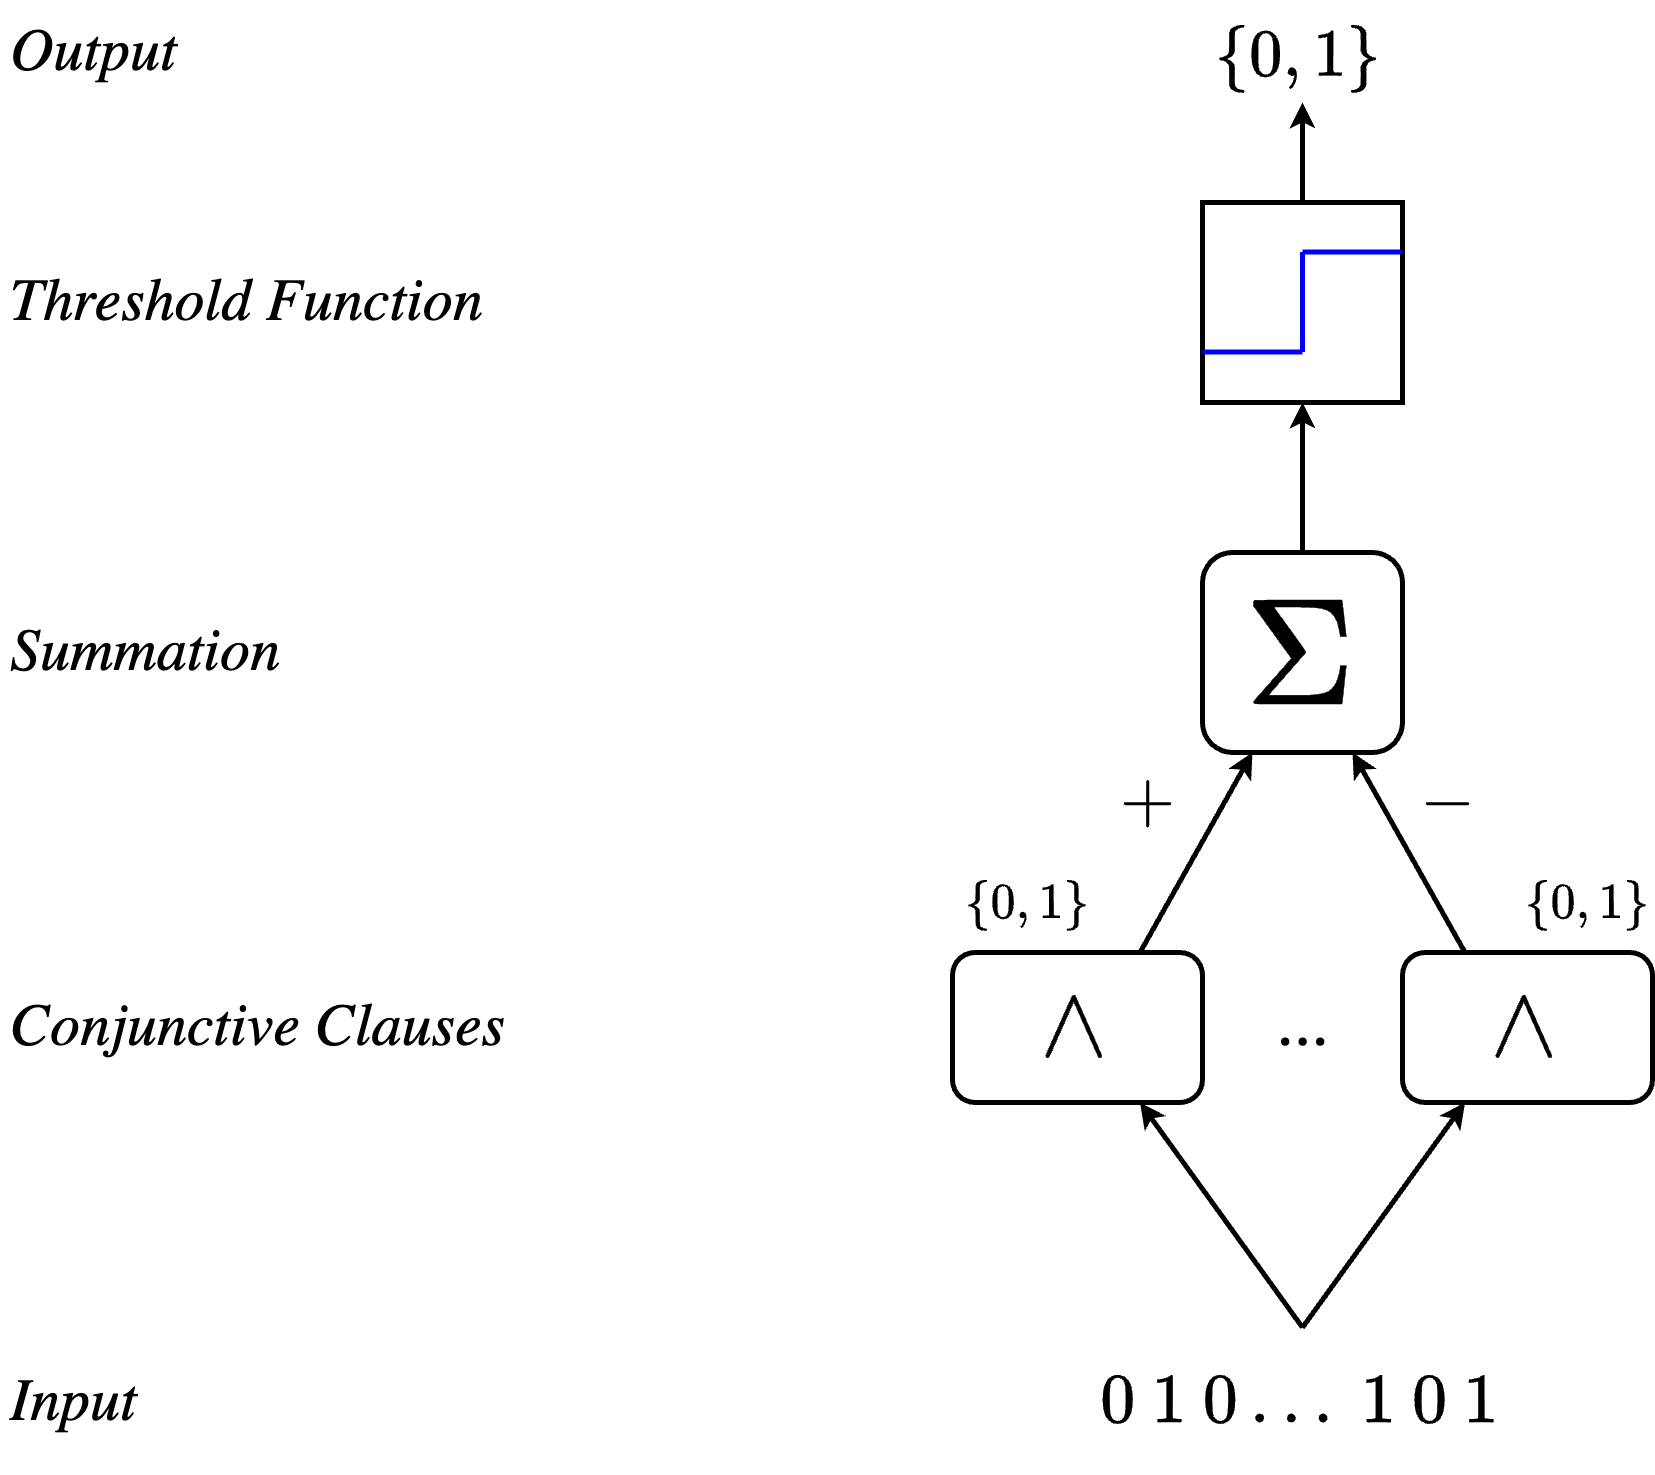
\includegraphics[width=0.65\linewidth]{inference-structure-v2.png}
    \caption{Inference structure for a binary-output Tsetlin Machine.}
    \label{fig:inference-structure}
\end{figure}

Let the input vector be
\[
X = (x_1, x_2, \dots, x_n) \in \{0,1\}^n.
\]
The full set of literals is
\[
L = \{x_1, \dots, x_n, \neg x_1, \dots, \neg x_n\},
\]
so that the number of literals is $|L| = 2n$. A clause $C_j$ is defined as a conjunction over a subset of literals,
\[
C_j = \bigwedge_{l_k \in L_j} l_k,
\]
where $L_j \subseteq L$. Each clause evaluates to $C_j \in \{0,1\}$ depending on whether all included literals are satisfied by the input.

Clauses are evenly divided into positive and negative polarity groups. Positive clauses vote for the target class, whereas negative clauses vote for the opposite class. For the weighted multi-class Tsetlin Machine (WMCTM) used in this work, the predicted class among $\zeta$ possible labels is computed as
\[
\hat{y} = 
\underset{i=1,\dots,\zeta}{\mathrm{argmax}}
\left(
\sum_{j=1}^{|C|/2} w_j^{+} C_j^{+}
-
\sum_{j=1}^{|C|/2} w_j^{-} C_j^{-}
\right),
\]
where $w_j^{+}$ and $w_j^{-}$ denote the learned clause weights for positive and negative polarity clauses, respectively.

Each literal is governed by a Tsetlin Automaton with $2N$ internal states. States $1,\dots,N$ correspond to excluding the literal from the clause, and states $N+1,\dots,2N$ correspond to including it. The automaton transitions between states through Type~I and Type~II feedback.

Type~I feedback reinforces patterns associated with correct classifications. It encourages clauses to include literals that frequently co-occur with the true class, while discouraging literals that introduce noise. The specificity parameter $s$ determines the balance between include-focused (Type~IA) and exclude-focused (Type~IB) updates.

Type~II feedback is activated when a clause contributes to a false positive. In such cases, the automata of included literals transition toward states that reduce the clause's likelihood of activating on similar incorrect inputs, thereby improving class discrimination.

Through these local, automaton-based updates, Tsetlin Machines learn structured logical patterns without relying on gradients or backpropagation. Throughout this work, we employ weighted multi-class Tsetlin Machines, as clause weighting has been shown to improve both discrimination and training behavior.


\section{Methodology}
In this section, we describe how knowledge distillation can be adapted to the Tsetlin Machine framework. We propose \textit{Distribution-Enhanced Knowledge Distillation} (DKD), a method that transfers information from a larger teacher Tsetlin Machine to a smaller student by leveraging both clause-level structure and distributional class information. Although Tsetlin Machines differ fundamentally from neural networks, DKD is inspired by classical distillation methods by using softened output distributions to guide learning.

The central idea behind DKD is that the teacher's most informative patterns should be transferred in a manner that improves generalization without increasing model size. Our approach integrates two complementary mechanisms: (1) \textit{clause initialization}, in which the student is seeded with a subset of influential clauses from the teacher, and (2) \textit{distributional supervision}, where the student receives additional guidance through probability distributions derived from the teacher's class-sum outputs.

To control the relative influence of these components, DKD introduces three interpretable hyperparameters:
\begin{enumerate}
    \item \textbf{Temperature} $(\tau \in (0,\infty))$: Regulates the entropy of teacher-derived probability distributions. High temperatures $(\tau > 1)$ produce softer distributions that highlight inter-class similarities, while low temperatures $(\tau < 1)$ sharpen the distribution around the predicted class. It is adapted from traditional knowledge distribution \cite{hinton2015distillingknowledgeneuralnetwork}.
    \item \textbf{Balance} $(\alpha \in [0,1])$: Determines the trade-off between ground-truth labels and teacher soft labels. When $\alpha = 1$, training reduces to standard TM learning; when $\alpha = 0$, training relies entirely on soft labels.
    \item \textbf{Weight transfer fraction} $(z \in [0,1])$: Controls how clauses are selected during initialization. Larger values emphasize high-weight clauses, and smaller values promote structural diversity among transferred clauses.
\end{enumerate}

We denote the teacher Tsetlin Machine as $TM_T$, the baseline student (trained without distillation) as $TM_S$, and the distilled student as $TM_D$. The models $TM_S$ and $TM_D$ are parametrically identical, enabling direct comparison of performance with and without distillation.

Traditional knowledge distillation in neural networks relies on logits or hidden-layer activations obtained through backpropagation. Tsetlin Machines do not produce such continuous internal representations. To address this limitation, we construct probability distributions from the teacher's unclamped class sums and combine them with clause transfer, resulting in a hybrid feature- and response-based form of distillation that enhances student accuracy while preserving interpretability and low latency~\cite{anjum2024novel, xu2023initializingmodelslargerones}. 

Following the standard KD workflow, the teacher is first trained for $E_T$ epochs. The student is then initialized with clauses selected from the teacher and trained for $E_S$ epochs using both hard labels and teacher-derived soft labels.

A key advantage of this approach is that the distilled model does not require the teacher during inference. The final student model is therefore suitable for deployment in memory- and power-constrained environments, including embedded systems and FPGA implementations where the larger teacher cannot be feasibly stored or executed.

\subsection{Clause Initialization}

The first component of our hybrid distillation framework operates prior to training the distilled model. Let the trained teacher Tsetlin Machine have a clause set $C_T$ and the student have a clause set $C_S$, denoted as $TM_T \ni C_T$ and $TM_S \ni C_S$, respectively. Since knowledge distillation aims to use a larger model to improve a smaller one, we assume $|C_T| > |C_S|$.

Previous studies have shown that smaller neural networks can be initialized with subsets of weights extracted from larger pretrained models~\cite{xu2023initializingmodelslargerones}. For Tsetlin Machines, the closest analogue to hidden-layer features is the set of propositional clauses. Because these clauses are independently learned patterns, they can be directly transferred between models. Thus, a student $TM_S$ can be initialized by copying up to $|C_S|$ clauses from the teacher $TM_T$, effectively providing pretrained structure. This constitutes a form of feature-based knowledge distillation.

To accomplish this, we introduce \textit{IntelligentTransfer} (Algorithm~\ref{algo:init-clauses}), which selects the top-$|C_S|$ teacher clauses based on a combination of influence and diversity. Let $\zeta$ denote the number of output classes, and let $z \in [0,1]$ represent the fraction of clauses allocated by weight, with $(1-z)$ representing the fraction allocated by diversity.

\DIFaddbegin \DIFadd{Algorithm \ref{algo:init-clauses} initializes the student Tsetlin Machine using clauses learned by the teacher model. Since clauses encode propositional patterns discovered during training, transferring a subset of these clauses allows the student to inherit useful structural bias before learning begins. The proposed selection strategy balances two complementary criteria: clause importance, measured by clause weight, and clause diversity, measured by the proportion of active Tsetlin Automata within each clause. This prevents the student from inheriting only highly weighted but redundant clauses, while still prioritizing influential patterns. The result is a compact initialization that preserves both discriminative strength and feature coverage.
}

\DIFaddend For weight-based selection, the teacher clauses in each class are sorted in descending order of their clause weights. Let $\lambda_{\text{weight}}$ denote the index set of the top $\lfloor z\cdot|C_S|\rfloor$ clauses. The remaining clause indices form the set $\Omega_{\text{remain}}$.

To compute diversity, we evaluate each remaining clause $(j,w_j) \in \Omega_{\text{remain}}$ for every class $k$. Let $A_j^k$ denote the set of Tsetlin Automata (TAs) associated with clause $j$ in class $k$. Define the TA activation ratio
\[
a_j = \frac{|A_j^k|_1}{|A_j^k|_0 + |A_j^k|_1},
\]
which reflects how often the clause includes its literals. Higher $a_j$ values indicate clauses that engage with a broader portion of the input space. Next, we normalize the clause weight,
\[
w'_j = \frac{w_j}{\max(W^k)},
\]
where $W^k$ is the set of clause weights for class $k$. Combining diversity and normalized weight yields
\[
v_j = w'_j \cdot a_j.
\]
Each score is stored in a set $D$, which is then sorted in descending order. The top $(|C_S| - n_{\text{direct}})$ indices from $D$ form the diversity-based clause set $\lambda_{\text{diverse}}$. The complete selection set is $\lambda_{\text{selected}} = \lambda_{\text{weight}} \cup \lambda_{\text{diverse}}$, which is transferred to the student.

Varying the weight-transfer parameter $z$ changes the balance between weight-focused and diversity-focused selection. When $z=0$, all transferred clauses are selected through diversity scoring. When $z=1$, selection is based solely on clause weight. In our experiments, $z=0.2$ provided an effective balance.

\DIFdelbegin %DIFDELCMD < \begin{algorithm}[H]
%DIFDELCMD < %%%
\DIFdelend \DIFaddbegin \begin{algorithm}[h]
\DIFaddend \caption{IntelligentTransfer: Clause Initialization for Student Tsetlin Machine}
\label{algo:init-clauses}
\begin{algorithmic}[1]
\Require $TM_T$: trained teacher Tsetlin Machine
\Require $TM_S$: student Tsetlin Machine
\Require $z \in [0,1]$: fraction of clauses selected by weight
\Function{IntelligentTransfer}{$TM_T, TM_S, z$}

\For{each class $k \in \{1,\ldots,\zeta\}$} 
    \State $W^k \gets$ clause weights of teacher for class $k$
    \State $A^k \gets$ TA states associated with each clause in class $k$
    \State $C_S^k \gets$ number of student clauses allocated to class $k$
    \State $\Omega \gets \{(j, W^k_j) : j = 1,\ldots,|W^k|\}$
    \State $n_{\text{direct}} \gets \max(1,\lfloor z \cdot C_S^k \rfloor)$
    \State Sort $\Omega$ in descending order by weight
    \State $\lambda_{\text{weight}} \gets$ first $n_{\text{direct}}$ indices from $\Omega$

    \State $\Omega_{\text{remain}} \gets \Omega \setminus \lambda_{\text{weight}}$
    \State $D \gets \emptyset$

    \For{each $(j, w_j)$ in $\Omega_{\text{remain}}$}
        \State $a_j \gets \frac{|A_j^k|_1}{|A_j^k|_0 + |A_j^k|_1}$
        \State $w'_j \gets \frac{w_j}{\max(W^k)}$
        \State $v_j \gets w'_j \cdot a_j$
        \State Append $(j, v_j)$ to $D$
    \EndFor

    \State Sort $D$ in descending order by score
    \State $n_{\text{diverse}} \gets C_S^k - n_{\text{direct}}$
    \State $\lambda_{\text{diverse}} \gets$ first $n_{\text{diverse}}$ indices from $D$

    \State $\lambda_{\text{selected}} \gets \lambda_{\text{weight}} \cup \lambda_{\text{diverse}}$

    \For{$m \gets 1$ to $|\lambda_{\text{selected}}|$}
        \State Transfer clause and weight from teacher at index $\lambda_{\text{selected}}[m]$ to student position $m$
    \EndFor
\EndFor

\EndFunction
\end{algorithmic}
\end{algorithm}

\subsection{Soft Label Generation}

\begin{figure}
    \centering
    
\includegraphics[width=0.75\linewidth]{soft-labels-flow.png}
    \caption{Visualization of the training process using soft labels.}
    \label{fig:soft-labels-flow}
\end{figure}

\begin{figure}[h]
    \centering
    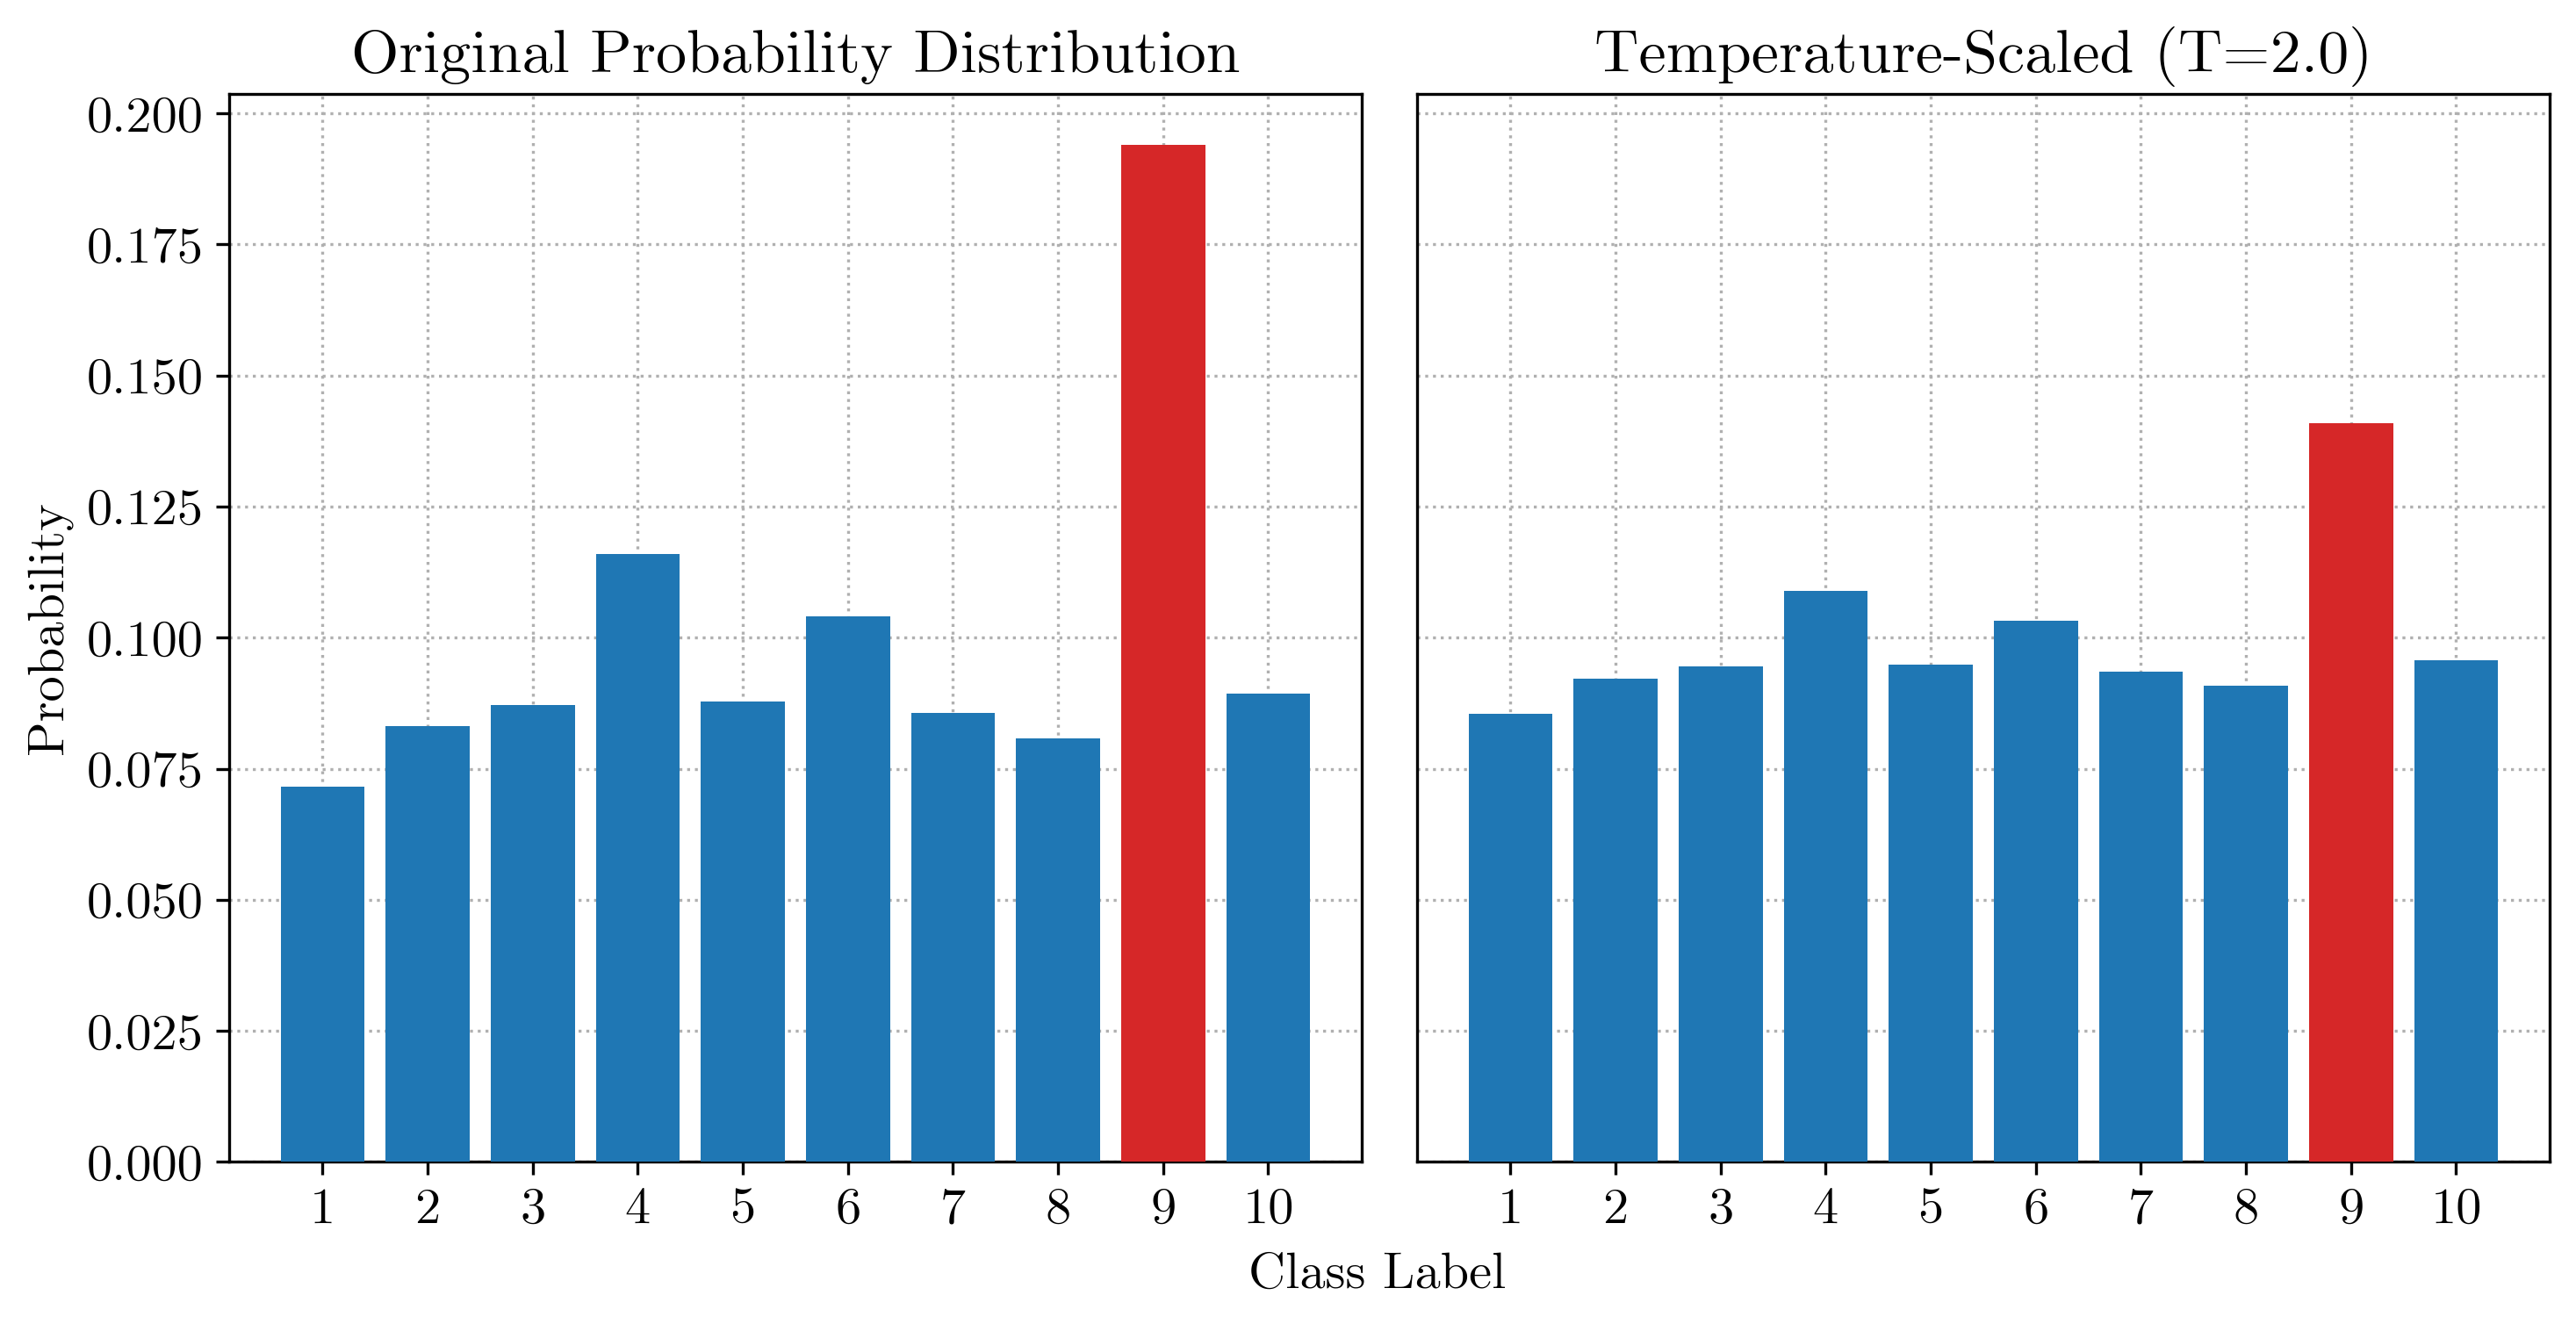
\includegraphics[width=0.65\linewidth]{pdist-ex-scaled.png}
    \caption{Fig. A1: Visualization of soft label probability distributions generated by 
    Algorithm \ref{algo:soft-labels}. Left: Temperature $\tau = 1.0$ (as generated). Center: $\tau = 2.0$ 
    (softer, more uniform). Right: $\tau = 0.5$ (sharper, peaked). The red bar 
    indicates the predicted class. Higher temperatures expose more information 
    about class relationships by flattening the distribution. Temperature scaling 
    is applied during training (Algorithm \ref{algo:fit-soft}), not during soft label generation.}
    \label{fig:pdist-ex-scaled}
\end{figure}

In order to teach the student TM to mimic the teacher, the student must be trained with a probability distribution over the teacher’s class predictions for each training sample. In traditional networks, these probability distributions (soft labels) are easily obtained from the output layer after applying the softmax function (see Figure~\ref{fig:pdist-ex-scaled}). The soft labels indicate for a data point $\mathbf{x}_i$ how likely it belongs to each class, with the class having the highest probability being the predicted class. On the left side of Figure~\ref{fig:pdist-ex-scaled} this is visualized; the selected class is shown in red. In TMs, however, we use discrete clause voting rather than continuous activations, so a different approach is required.

Recall that in a traditional multi-class Tsetlin Machine, classification is determined by computing class sums (the sum of positive and negative weighted clause votes). Let $|C|$ be the number of clauses and $\zeta$ the number of classes in a Tsetlin Machine. For a weighted multi-class Tsetlin Machine, the class sums $C \in \mathbb{R}^\zeta$ over the $\zeta$ classes are computed as shown in Equation~\eqref{eq:csums-general}:

\begin{equation}
\label{eq:csums-general}
\mathbb{C}_{k} = \sum_{j=1}^{|C|/2} w^+_{j,k}C_{j,k}^{+} \;-\; \sum_{j=1}^{|C|/2} w^-_{j,k}C_{j,k}^{-}, \quad \forall k \in \{1, \dots, \zeta\}.  % EDIT: added spacing around minus
\end{equation}

In order to convert these class sums into valid soft labels, we apply the procedure given in Algorithm~\ref{algo:soft-labels}. These class sums contain valuable information about the teacher’s confidence across all classes, not just the top class. However, they cannot be directly used as probability distributions because they can be negative (due to negative clause votes), they are unbounded, and may not sum to one.

\DIFdelbegin %DIFDELCMD < \begin{algorithm}[H]
%DIFDELCMD < %%%
\DIFdelend \DIFaddbegin \DIFadd{Algorithm \ref{algo:soft-labels} converts raw, unclamped class sums produced by a teacher Tsetlin Machine into probability distributions suitable for knowledge distillation. Unlike neural networks, Tsetlin Machines produce discrete and potentially unbounded class sums that may be negative and are not directly comparable across samples. The algorithm therefore applies a sequence of transformations to preserve relative class confidence while ensuring numerical stability: class sums are first shifted to remove negative values, then normalized on a per-sample basis, and finally transformed into a probability distribution using a temperature-scaled softmax. In degenerate cases where all class sums are equal, the procedure yields a uniform distribution, reflecting maximal uncertainty in the teacher’s prediction.
}

\DIFadd{To address these issues, Algorithm~\ref{algo:soft-labels} applies a sequence of transformations designed to preserve relative class confidence while ensuring numerical stability. First, a per sample shifting operation removes negative values without altering the ordering of class scores. Next, per sample normalization scales class sums to a comparable range, preventing dominance by samples with large magnitude scores. The exponential transformation emphasizes relative differences between classes, and the final normalization step produces valid probability distributions that sum to one. Together, these steps enable stable and meaningful soft labels suitable for distillation in the absence of continuous logits or backpropagation.
}

\begin{algorithm}[h]
\DIFaddend \caption{Generate Soft Labels from Tsetlin Machine Class Sums}
\label{algo:soft-labels}
\begin{algorithmic}[1]
\Require $\mathbb{C} \in \mathbb{R}^{N \times \zeta}$: raw (unclamped) class sums for $N$ examples across $\zeta$ classes
\Function{GetSoftLabels}{$\mathbb{C}$}
  \Comment{Phase 1: Make class sums non-negative}
  \State $c_{\min}^i = \min_{j \in \{1,\dots,\zeta\}} \mathbb{C}_{ij}, \quad \forall i = 1,\dots,N$
  \State $\hat{\mathbb{C}}_{ij} = \mathbb{C}_{ij} - c_{\min}^i, \quad \forall i,j$  
   \Comment{Now $\hat{\mathbb{C}}_{ij} \ge 0$}
  \\
  \Comment{Phase 2: Normalize per example to [0,1]}
  \State $m_i = \max_{j \in \{1,\dots,\zeta\}} \hat{\mathbb{C}}_{ij}, \quad \forall i$
  \If{$m_i > 0$}
    \State $\bar{\mathbb{C}}_{ij} = \hat{\mathbb{C}}_{ij} / m_i, \quad \forall j$  
     \Comment{So that $\bar{\mathbb{C}}_{ij} \in [0,1]$ and the maximum equals 1}
  \Else
    \State $\bar{\mathbb{C}}_{ij} = 0, \quad \forall j$  
     \Comment{In the degenerate case where all raw sums are equal}
  \EndIf
  \\
  \Comment{Phase 3: Exponentiate and normalize to produce a probability distribution}
  \State $P_{ij} = \exp\left(\bar{\mathbb{C}}_{ij} / \tau\right), \quad \forall i,j$  % EDIT: make temperature explicit
  \State $S_{ij} = \displaystyle \frac{P_{ij}}{\sum_{k=1}^{\zeta} P_{ik}}, \quad \forall i,j$
  \State \Return $S \in \mathbb{R}^{N \times \zeta}$
\EndFunction
\end{algorithmic}
\end{algorithm}

Here $S_{ij}$ can be interpreted as the teacher’s estimated probability $\mathbb{P}(y_i = j \mid \mathbf{x}_i)$. Each row $S_i$ is a valid probability distribution over classes. The optional temperature parameter $\tau > 0$ (which defaults to 1 if not explicitly used) allows controlling the softness of the distribution during distillation.

For example, suppose for a 3-class TM we obtain raw class sums  
\[
\mathbb{C} = [-50,\;120,\;-30].
\]  
Then Phase 1 (shift) yields  
\[
\hat{\mathbb{C}} = [0,\;170,\;20].
\]  
Phase 2 (normalize) yields  
\[
\bar{\mathbb{C}} = [0,\;1.0,\;0.118],
\]  
Phase 3 (softmax with $\tau = 1$) yields  
\[
P = [\exp(0),\;\exp(1.0),\;\exp(0.118)] = [1,\;2.718,\;1.125],
\]  
and finally the normalized soft labels are  
\[
S \approx [0.204,\;0.554,\;0.229].
\]  
Thus the teacher assigns approximately 55.4\% probability to class 2, 22.9\% to class 3, and 20.4\% to class 1 — not just the single top class but a full distribution reflecting confidence and relative class plausibility.

Our approach differs from standard logit-based softmax (often used in neural networks) by introducing shifting and scaling before exponentiation. These steps ensure non-negativity, avoid numerical instability due to large or negative sums, and preserve relative differences in class votes. We apply any temperature scaling only during distillation, not during soft‑label generation, which simplifies reuse of soft labels across different training regimes.

This procedure enables the student model to learn not only the teacher’s top prediction but its confidence structure across classes, potentially transferring richer “dark knowledge” as shown to improve generalization in various distillation settings (e.g., knowledge distillation literature).  

\subsection{Improved Training} 

To use the soft labels generated by the teacher in Algorithm~\ref{algo:soft-labels}, we modify the standard Tsetlin Machine update step. \DIFaddbegin \DIFadd{Algorithm \ref{algo:soft-labels} describes the training procedure for the distilled Tsetlin Machine using both hard labels and soft labels provided by the teacher. During training, the student receives standard clause feedback derived from ground-truth labels, while additional guidance is incorporated through probability distributions generated from the teacher’s class sums. A balance parameter controls the relative influence of hard and soft supervision, allowing the student to learn both the target labels and the teacher’s confidence structure. This approach preserves the original Tsetlin Machine learning dynamics while enriching the training signal with distribution-level information.
}

\DIFaddend Training consists of two phases: reinforcing the positive class and reinforcing the negative classes. Recall that a multi-class Tsetlin Machine can be viewed as a team of $\zeta$ TMs, one for each class. In standard multi-class TM training, Type I feedback is sent to the true class $c$, and Type II feedback is sent to a random negative class $\neq c$.

We propose a novel fit method for use in Tsetlin Machines, described in Algorithm~\ref{algo:fit-soft}. As in traditional TM training, the algorithm takes training data $X \in \mathbb{R}^{N \times n}$, true labels $y \in \mathbb{R}^N$, the number of training examples $N$, and the number of epochs $E$. We introduce three additional parameters: soft labels $S \in \mathbb{R}^{N \times \zeta}$, balance $\alpha \in [0,1]$, and distribution temperature $\tau \in (0,\infty)$. The balance parameter $\alpha$ controls the influence of soft labels in training, while the temperature $\tau$ adjusts the entropy of the soft labels. Figure~\ref{fig:soft-labels-flow} illustrates the data pathway for training the distilled model.

First, for each epoch $e$ and example $i$, the soft label distributions are adjusted by temperature $\tau^2$ and re-normalized. This modifies the entropy of the soft labels: a higher $\tau>1$ increases entropy, moving the distribution toward uniform, while $\tau<1$ decreases entropy, emphasizing the true class. This effect is shown in Figure~\ref{fig:pdist-ex-scaled}.

\DIFdelbegin %DIFDELCMD < \begin{algorithm}[H]
%DIFDELCMD < %%%
\DIFdelend \DIFaddbegin \DIFadd{In Algorithm~\ref{algo:fit-soft}, Type I feedback is applied to the true class $y_i=c$ with probability $\alpha$, allowing the student to learn from ambiguous examples and mimic the teacher. For each class $k$, the base feedback probability $\phi = (1-\alpha) p_{i,k}$ is computed. Classes with $\phi < 0.001$ are skipped for efficiency. The feedback type is determined by the soft label: $p_{i,k} > 0.5$ indicates a possible positive class (Type I), otherwise Type II. The feedback probability is then adjusted by confidence and temperature before stochastic application. This process is repeated for each class, example, and epoch, enabling the distilled model to integrate both teacher soft labels and ground truth information.
}

\begin{algorithm}[htbp]
\DIFaddend \caption{Tsetlin Machine fit method using soft label distributions}
\label{algo:fit-soft}
\begin{algorithmic}[1]
\Require $X\in\mathbb{R}^{N \times n}$: Training examples
\Require $y\in\mathbb{R}^{N}$: True class labels
\Require $S\in\mathbb{R}^{N \times \zeta}$: Teacher probability distributions (soft labels)
\Require $N$: Number of training examples
\Require $E$: Number of epochs
\Require $\alpha \in [0,1]$: Balance between hard/soft labels (0=pure soft, 1=pure hard)
\Require $\tau \in (0,\infty)$: Temperature for sharpening/softening distributions

\Function{FitEnhanced}{$X, y, S, N, E, \alpha, \tau$}
    \For{each epoch $e \in \{1,\ldots,E\}$}
        \For{each example $i \in \{1,\ldots,N\}$}
            \State $c \gets y_i$ \Comment{True class label for current example}
            \State $p_i \gets S_i^{1/\tau^2}$ \Comment{Apply temperature scaling}
            \State $p_i \gets p_i / \sum p_i$ \Comment{Renormalize to probability distribution}

            \Comment{Phase 1: Hard Label Training}
            \State $u \sim \mathcal{U}(0,1)$
            \If{$u \leq \alpha$}
                \State $\text{TM}_c.\text{update}(X_i, \texttt{Type I})$
            \EndIf

            \Comment{Phase 2: Soft Label Training}
            \For{each class $k \in \{1,\ldots,\zeta\}$}
                \If{$k = c$ \textbf{and} $\alpha > 0$} \Comment{Skip true class if already trained with hard labels}
                    \State \textbf{continue}
                \EndIf
                \State $\phi \gets (1 - \alpha) \, p_{i,k}$ \Comment{Base feedback probability}
                \If{$\phi < 0.001$} \Comment{Skip unlikely classes}
                    \State \textbf{continue}
                \EndIf

                \If{$p_{i,k} > 0.5$}
                    \State $f \gets \texttt{Type I}$ \Comment{Positive feedback}
                    \State $\phi \gets \phi (1 + p_{i,k} \tau)$
                \Else
                    \State $f \gets \texttt{Type II}$ \Comment{Negative feedback}
                    \State $\phi \gets \phi (1 + (1 - p_{i,k}) \tau)$
                \EndIf

                \State $u \sim \mathcal{U}(0,1)$ \Comment{Independent random draw}
                \If{$u \leq \phi$}
                    \State $\text{TM}_k.\text{update}(X_i, f)$
                \EndIf
            \EndFor
        \EndFor
    \EndFor
\EndFunction
\end{algorithmic}
\end{algorithm}




\DIFdelbegin \DIFdel{In Algorithm~\ref{algo:fit-soft}, Type I feedback is applied to the true class $y_i=c$ with probability $\alpha$, allowing the student to learn from ambiguous examples and mimic the teacher. For each class $k$, the base feedback probability $\phi = (1-\alpha) p_{i,k}$ is computed. Classes with $\phi < 0.001$ are skipped for efficiency. The feedback type is determined by the soft label: $p_{i,k} > 0.5$ indicates a possible positive class (Type I), otherwise Type II. The feedback probability is then adjusted by confidence and temperature before stochastic application. This process is repeated for each class, example, and epoch, enabling the distilled model to integrate both teacher soft labels and ground truth information.
}%DIFDELCMD < 

%DIFDELCMD < %%%
\DIFdelend \section{Experiment and Results}
In this section, we explore how using a feature- and response-based teacher-student knowledge distillation model affects accuracy and performance across several datasets. We test both approaches described in the previous section to determine which performs best. For both approaches, we compare training and testing accuracy and runtime to evaluate effectiveness. All experiments are conducted using a parallel Tsetlin Machine implementation~\footnote{https://github.com/ckinateder/pyTsetlinMachineParallel}. 

\subsection{Datasets}

We use four standard benchmark datasets: MNIST, KMNIST, EMNIST, and IMDB. 

\subsection{Dataset Descriptions} \label{dataset-desc}

\subsubsection{MNIST}
MNIST (Modified National Institute of Standards and Technology)~\cite{lecun1998gradient} is a widely used dataset containing 70,000 samples of handwritten digits. It is split into 60,000 training images and 10,000 testing images. Each image is a grayscale digit in $\{0,1,...,9\}$ and has size $28 \times 28$ pixels. 

\subsubsection{Kuzushiji-MNIST (KMNIST)}
Kuzushiji-MNIST~\cite{kmnist} contains 70,000 grayscale images of historical Japanese characters, with 60,000 training images and 10,000 test images. Each image has size $28 \times 28$ pixels and there are 10 classes. KMNIST provides an alternative to MNIST for evaluating classification performance on non-Latin characters.

\subsubsection{Extended-MNIST (EMNIST)}
EMNIST~\cite{DBLP:EMNIST} contains 145,600 grayscale $28 \times 28$ images. It consists of 124,800 training images and 20,800 testing images across 26 classes, one for each letter of the alphabet.

\subsubsection{IMDB}
The IMDB dataset~\cite{maas-EtAl:2011:ACL-HLT2011} is a text classification dataset for sentiment analysis over movie reviews. It contains 25,000 highly polarized movie reviews for training and 25,000 for testing. There are two classes: positive and negative. 

\subsection{Dataset Preprocessing}
For the image datasets, all grayscale images are binarized at a threshold of $75/255$ (0.3 normalized). This threshold provides a balance between preserving edge information and reducing noise across all three image datasets. Pixels with intensity $\leq 75$ are set to 0, and pixels with intensity $>75$ are set to 1.

IMDB textual data is preprocessed into n-grams and converted into bit representations, resulting in a total of 5,000 features per sample.

\begin{table}
\centering
\caption{Dataset Information}
\begin{tabular}{|l|c|c|c|c|c|}
\hline
Dataset & $|X_{train}|$ & $|X_{test}|$ & $|L|$ & $\zeta$ & Type\\
\hline
EMNIST & 124800 & 20800 & 784 & 26 & Image \\\hline
MNIST & 60000 & 10000 & 784 & 10 & Image \\\hline
KMNIST & 60000 & 10000 & 784 & 10 & Image \\\hline
IMDB & 25000 & 25000 & 5000 & 2 & Text \\
\hline
\end{tabular}
\label{tab:dataset-size}
\end{table}


\subsection{Experiment Design}

Our experiments follow a knowledge distillation scenario similar to neural networks. We have a student model $TM_S$, a teacher model $TM_T$, and a distilled model $TM_D$. All three models share the same parameters except for the number of clauses. The student model is assigned fewer clauses than the teacher (in our experiments, between 2 and 10 times fewer), and the distilled model has the same number of clauses as the student model. The student model serves as a baseline for what the distilled model would achieve without our proposed algorithms. Because the student and distilled models have the same size, they should have roughly the same speed.

Let $E_S$ and $E_T$ denote the number of student and teacher epochs, respectively. Let $E_{T+S} = E_T + E_S$ denote the total number of epochs. The choice of epoch counts (Table~\ref{tab:hyperparams-dkd}) was determined through preliminary convergence analysis on validation data.

First, the student model $TM_S$ is trained on the dataset for $E_{T+S}$ epochs, providing a baseline of expected accuracy for a Tsetlin Machine with $C_S$ clauses and $E_{T+S}$ epochs. Next, the teacher model $TM_T$ is trained with $C_T$ clauses for $E_{T+S}$ epochs.

Once the baselines are established, we reinitialize the teacher model $TM_T$ from the checkpoint at $E_T$ epochs to avoid giving the distilled model an unfair advantage. We then initialize the distilled model $TM_D$ with the clauses of the trained teacher using Algorithm~\ref{algo:init-clauses}. Soft labels are generated from the teacher over the training dataset using Algorithm~\ref{algo:soft-labels}. Finally, the distilled model is trained for $E_S$ epochs on the training dataset and the soft labels from the teacher using Algorithm~\ref{algo:fit-soft}. Because Tsetlin Machines are stochastic, each experiment is repeated $K$ times and results are averaged. \DIFaddbegin \DIFadd{We report mean and standard deviation across runs; formal hypothesis testing is not performed, and observed improvements should therefore be interpreted as consistent empirical trends rather than statistically certified gains.
}\DIFaddend 

\DIFaddbegin \DIFadd{The experimental design focuses on isolating the effect of distribution-enhanced supervision and clause-level transfer under fixed architectural settings. Accordingly, comparisons are limited to teacher, student, and distilled models that share identical hyperparameters aside from clause count. Alternative approaches such as extended training of smaller Tsetlin Machines, weighted or regularized TMs, and explicit clause pruning without distillation are not evaluated experimentally in this study. These comparisons represent important directions for future work.
}

\DIFaddend For data collection, we measure average accuracies over $E_{T+S}$ epochs. Training and testing times are recorded for the student and teacher baselines over $E_{T+S}$ epochs, and for the distilled model over $E_S$ epochs. This reflects that the distilled model begins training after $E_T$ epochs with a smaller architecture than the teacher. The time for generating soft labels, clause outputs, and applying PCD is not included, as it is a one-time cost approximately equal to the time of one training epoch.

Hyperparameters for our distribution-enhanced experiments are shown in Table~\ref{tab:hyperparams-dkd}. Temperature selection ($\tau$ in Table~\ref{tab:hyperparams-dkd}) was determined through preliminary grid search experiments over the range $[1.0, 2.0, 3.0, 4.0, 5.0]$. We found that $\tau \in [3.0, 4.0]$ consistently produced the best results across datasets, outperforming the vanilla softmax ($\tau = 1.0$). This suggests that softer distributions, which reveal more information about class relationships, are particularly valuable for Tsetlin Machines, likely because they help guide discrete propositional logic clauses toward capturing inter-class boundaries more effectively. 

Overall, we observe across all datasets that \DIFdelbegin \DIFdel{our }\DIFdelend \DIFaddbegin \DIFadd{the }\DIFaddend proposed knowledge distillation approach \DIFdelbegin \DIFdel{significantly improves accuracy and performance in the distilled model. The influence of the teacher on the distilled model is also visible in the included clause literals}\DIFdelend \DIFaddbegin \DIFadd{consistently improves the accuracy of the distilled model relative to a non-distilled student under identical architectural constraints, while maintaining comparable training and inference costs}\DIFaddend . 

\begin{table*}
\centering
\caption{Experiment Hyperparameters (DKD)}
\begin{tabular}{|l|c|c|c|c|c|c|c|c|c|c|c|c|}
\hline
Dataset & $|C_T|$ & $|C_S|$ & $T_T$ & $T_S$ & $s_T$ & $s_S$ & $\tau$ & $\alpha$ & $z$ & $E_T$ & $E_S$ & $K$ \\
\hline
EMNIST & 1000 & 100 & 100 & 100 & 4.0 & 4.0 & 4.0 & 0.5 & 0.2 & 120 & 240 & 10 \\\hline
MNIST & 1000 & 100 & 10 & 10 & 4.0 & 4.0 & 3.0 & 0.5 & 0.3 & 120 & 240 & 10 \\\hline
KMNIST & 2000 & 200 & 100 & 100 & 8.2 & 8.2 & 4.0 & 0.5 & 0.3 & 120 & 240 & 10 \\\hline
IMDB & 8000 & 4000 & 6000 & 6000 & 7.0 & 7.0 & 3.0 & 0.5 & 0.2 & 30 & 60 & 8 \\
\hline
\end{tabular}
\label{tab:hyperparams-dkd}
\end{table*}


\subsection{Training Accuracy and Performance Analysis} \label{sec:trapa}

\begin{table*}
\centering
\caption{Training Results}
\begin{tabular}{|l|c|c|c|c|c|c|}
\hline
Dataset & $Acc'_T$ & $\mathcal{T}'_T$ & $Acc'_S$ & $\mathcal{T}'_S$ & $Acc'_D$ & $\mathcal{T}'_D$ \\
\hline
MNIST & 97.65 \newline $\pm$ 0.07 & 0.70 \newline $\pm$ 0.01 & 90.63 \newline $\pm$ 0.13 & 0.26 \newline $\pm$ 0.00 & 95.25 \newline $\pm$ 0.07 & 0.24 \newline $\pm$ 0.00 \\\hline%\hdashline
KMNIST & 98.10 \newline $\pm$ 0.03 & 1.69 \newline $\pm$ 0.05 & 92.46 \newline $\pm$ 0.03 & 0.34 \newline $\pm$ 0.00 & 94.66 \newline $\pm$ 0.04 & 0.36 \newline $\pm$ 0.00 \\\hline%\hdashline
EMNIST & 86.88 \newline $\pm$ 0.09 & 3.15 \newline $\pm$ 0.02 & 79.35 \newline $\pm$ 0.06 & 0.62 \newline $\pm$ 0.00 & 83.20 \newline $\pm$ 0.06 & 0.67 \newline $\pm$ 0.00 \\\hline%\hdashline
IMDB & 99.41 \newline $\pm$ 0.07 & 28.95 \newline $\pm$ 0.42 & 98.39 \newline $\pm$ 0.24 & 17.07 \newline $\pm$ 0.35 & 98.96 \newline $\pm$ 0.13 & 9.35 \newline $\pm$ 0.29 \\
\hline
\end{tabular}
\label{tab:train-table-dkd}
\end{table*}


\begin{figure}[h]
    \centering
    \begin{subfigure}[b]{0.49\linewidth}
        \centering
        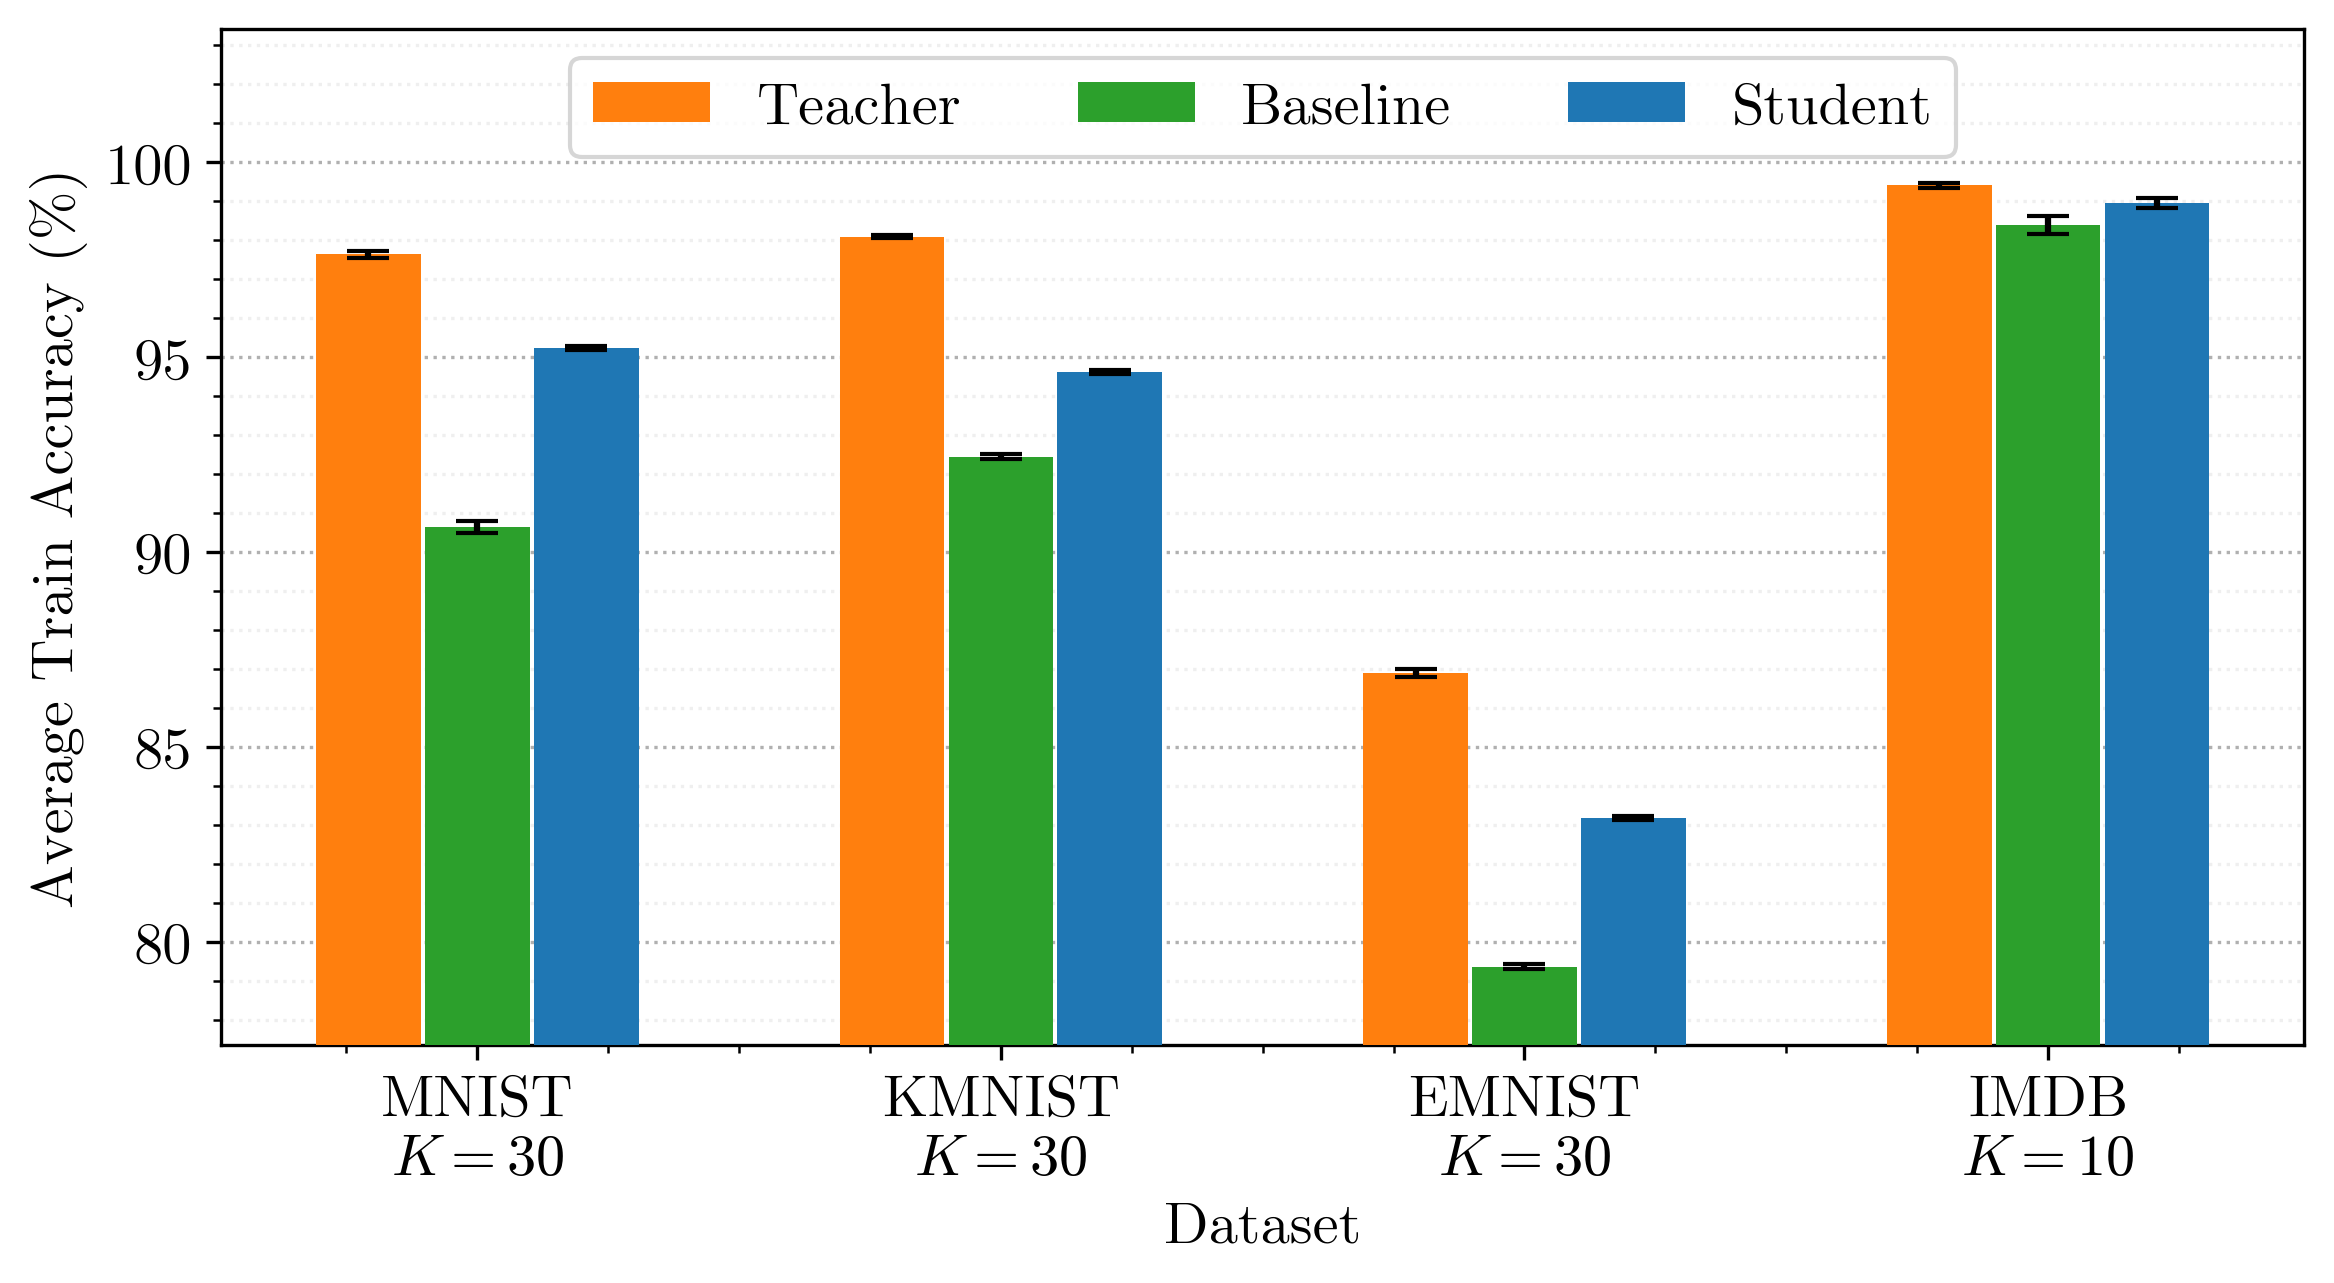
\includegraphics[width=\linewidth]{combined_train_acc.png}
        \caption{Average training accuracy $Acc'$ on each dataset using DKD.}
        \label{fig:train-acc-combined}
    \end{subfigure}
    \hfill
    \begin{subfigure}[b]{0.49\linewidth}
        \centering
        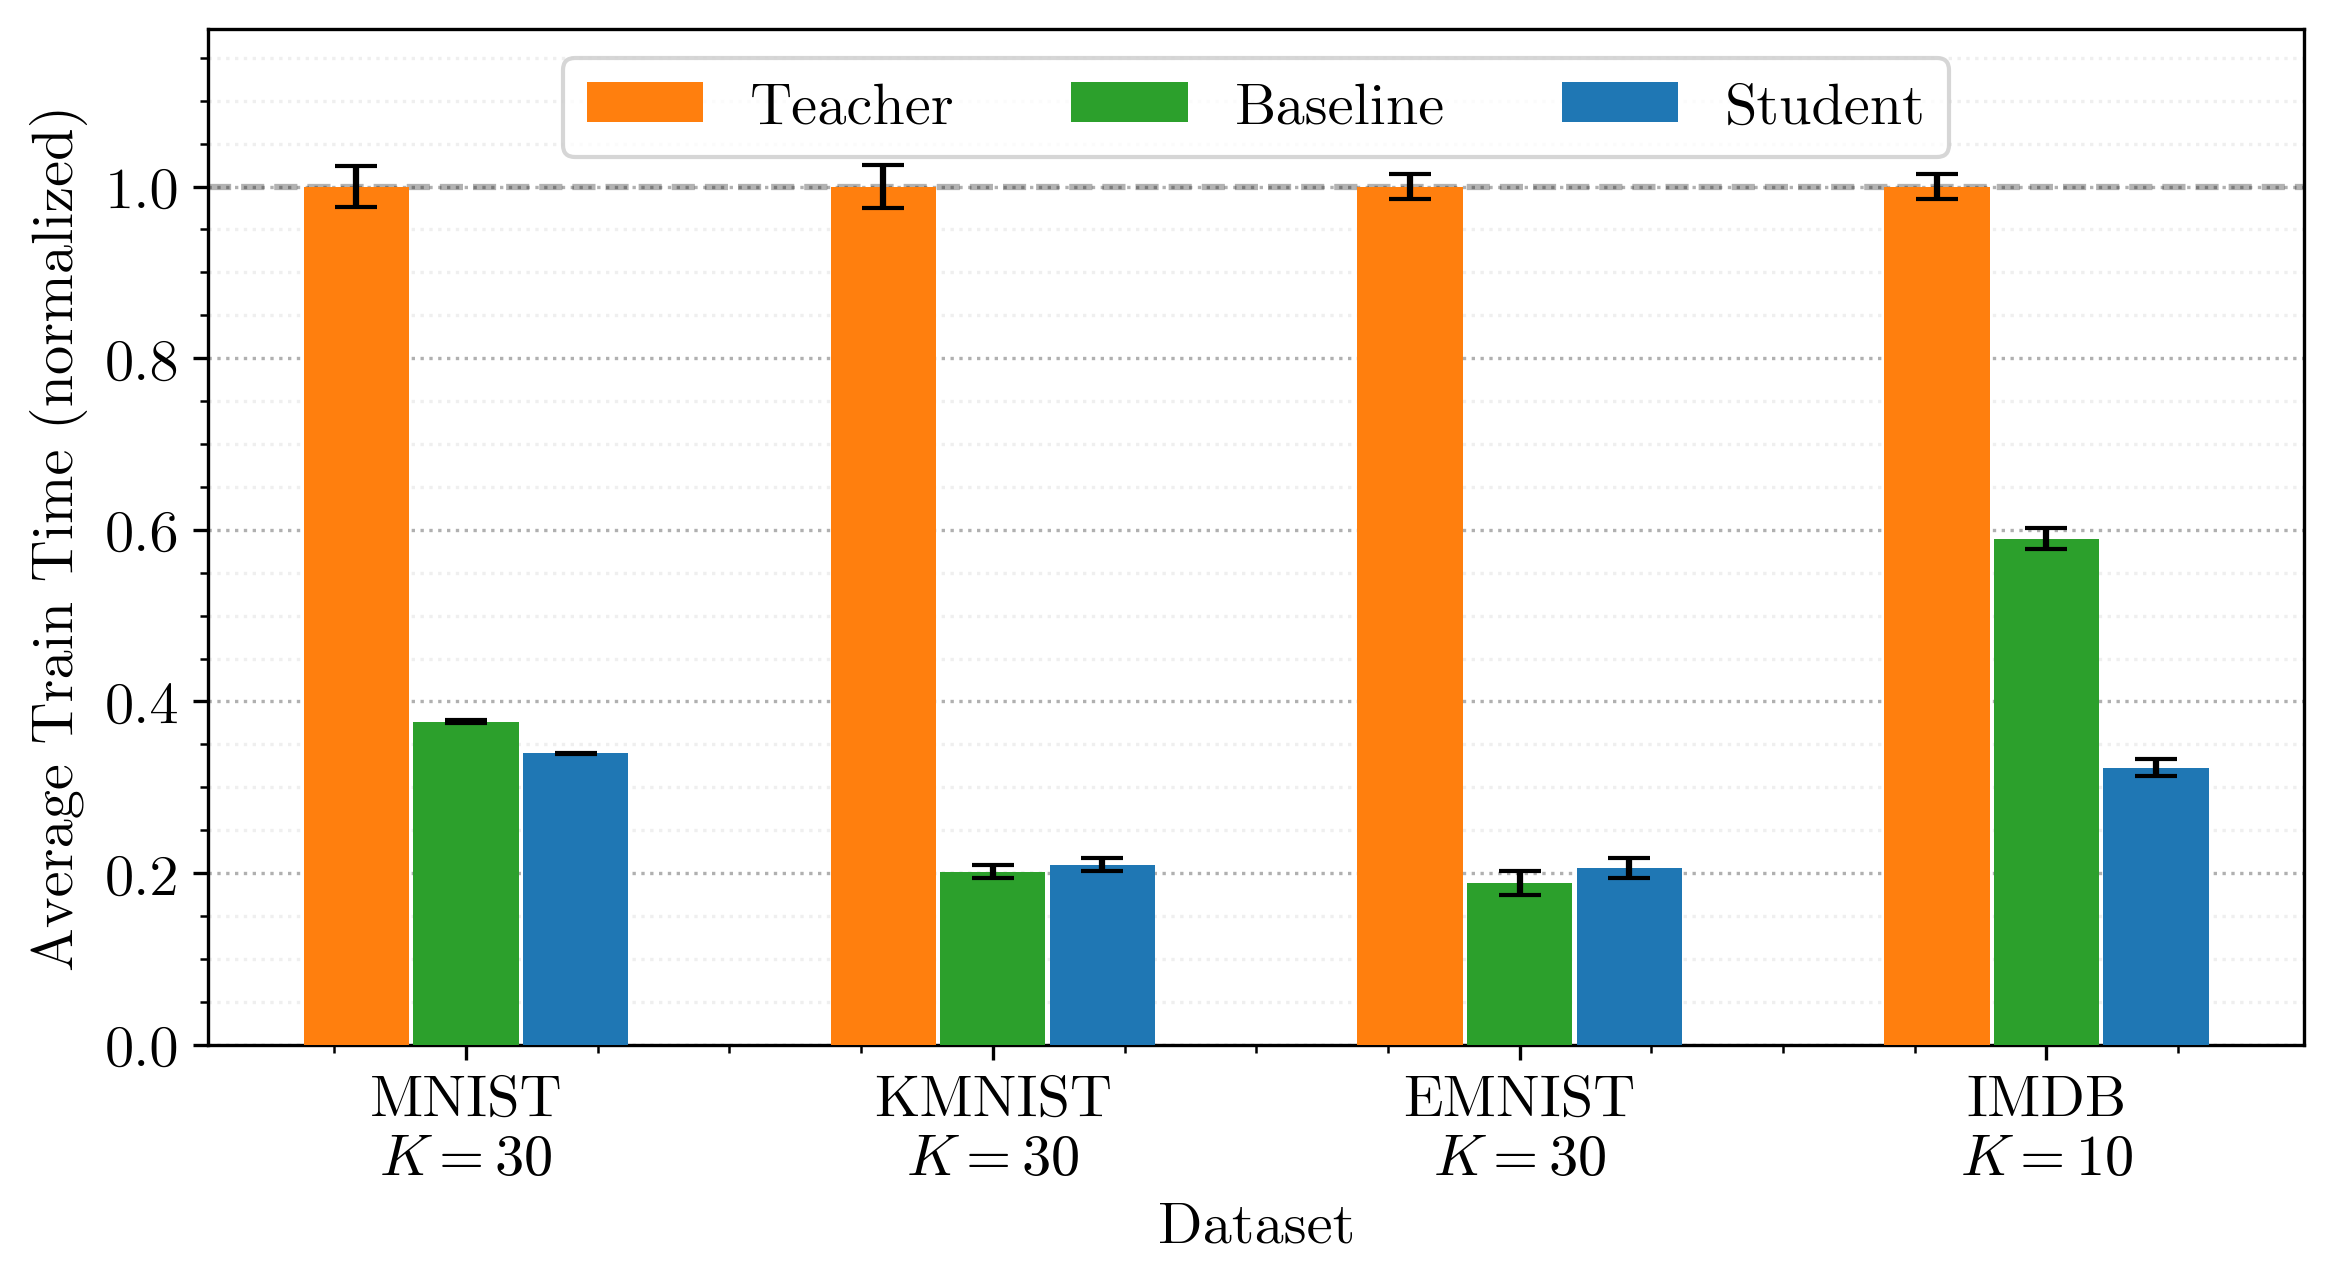
\includegraphics[width=\linewidth]{combined_train_time.png}
        \caption{Average epoch training time $\mathcal{T}'$ on each dataset using DKD.}
        \label{fig:train-time-combined}
    \end{subfigure}
    \caption{Training accuracy and epoch time on each dataset using DKD.}
    \label{fig:train-acc-time-combined}
\end{figure}

The experimental results indicate that \DIFdelbegin \DIFdel{using }\DIFdelend teacher-student knowledge distillation \DIFdelbegin \DIFdel{can significantly improve }\DIFdelend \DIFaddbegin \DIFadd{consistently improves }\DIFaddend the training accuracy of a smaller model with minimal overhead. Clause transfer from the teacher to the distilled model, combined with distribution-enhanced fitting, allows the distilled model to achieve higher accuracy without increasing training time. These results are summarized in Table~\ref{tab:train-table-dkd} and illustrated in Figures~\ref{fig:train-acc-combined} and~\ref{fig:train-time-combined}.

The average training times in Figure~\ref{fig:train-time-combined} are normalized to allow fair comparison across datasets of different sizes. For the EMNIST dataset, training accuracy improves by nearly 4 percentage points compared to the baseline student model, while maintaining similar epoch times. This is further illustrated in Figures~\ref{fig:train-acc-emnist} and~\ref{fig:train-time-combined}. 

Training efficiency can also be visualized in an efficiency plot (Figure~\ref{fig:train-eff-emnist}). Points to the left of the diagonal line represent a ``free lunch'' region, where accuracy increases without a proportional increase in execution time. This reflects the core idea of knowledge distillation: improving accuracy without additional training cost. \DIFaddbegin \DIFadd{This visualization is intended as an intuitive comparison rather than a formal efficiency guarantee.
}\DIFaddend 

\begin{figure}[h]
    \centering
    \begin{subfigure}[b]{0.48\linewidth}
        \centering
        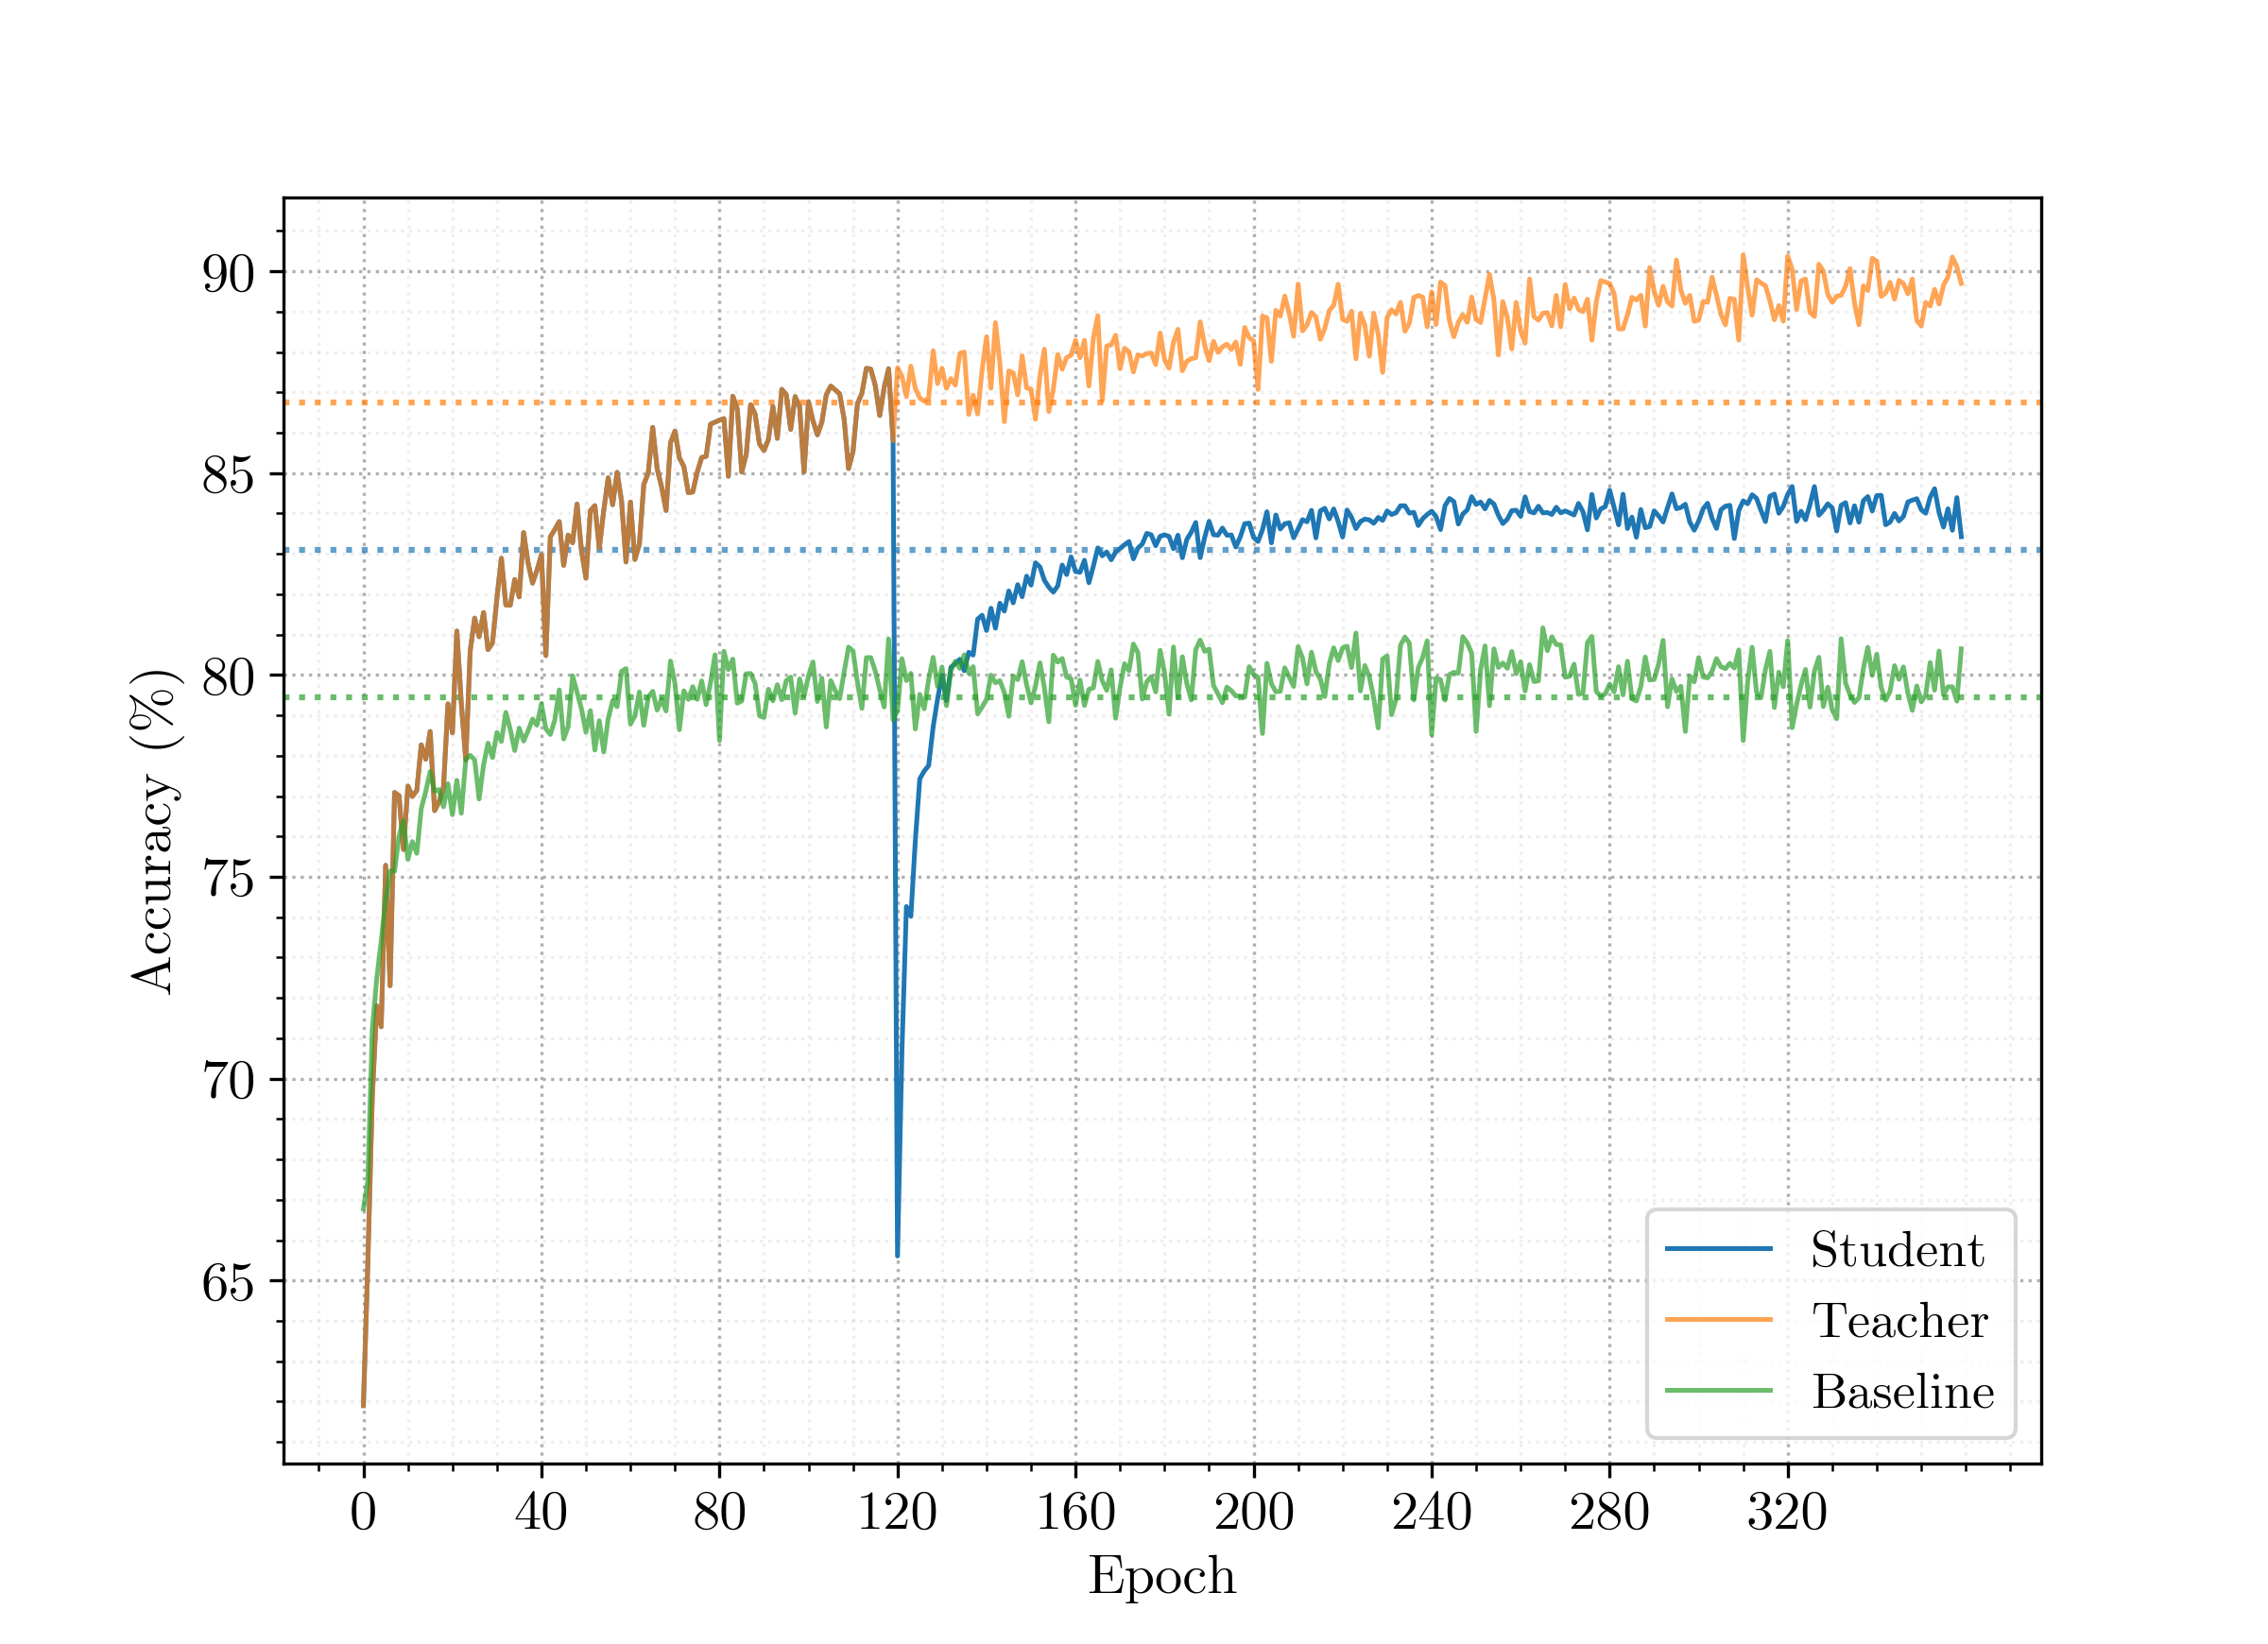
\includegraphics[width=\linewidth]{EMNIST_train_accuracy.png}
        \caption{Training accuracy $Acc'$ on EMNIST using DKD.}
        \label{fig:train-acc-emnist}
    \end{subfigure}
    \hfill
    \begin{subfigure}[b]{0.48\linewidth}
        \centering
        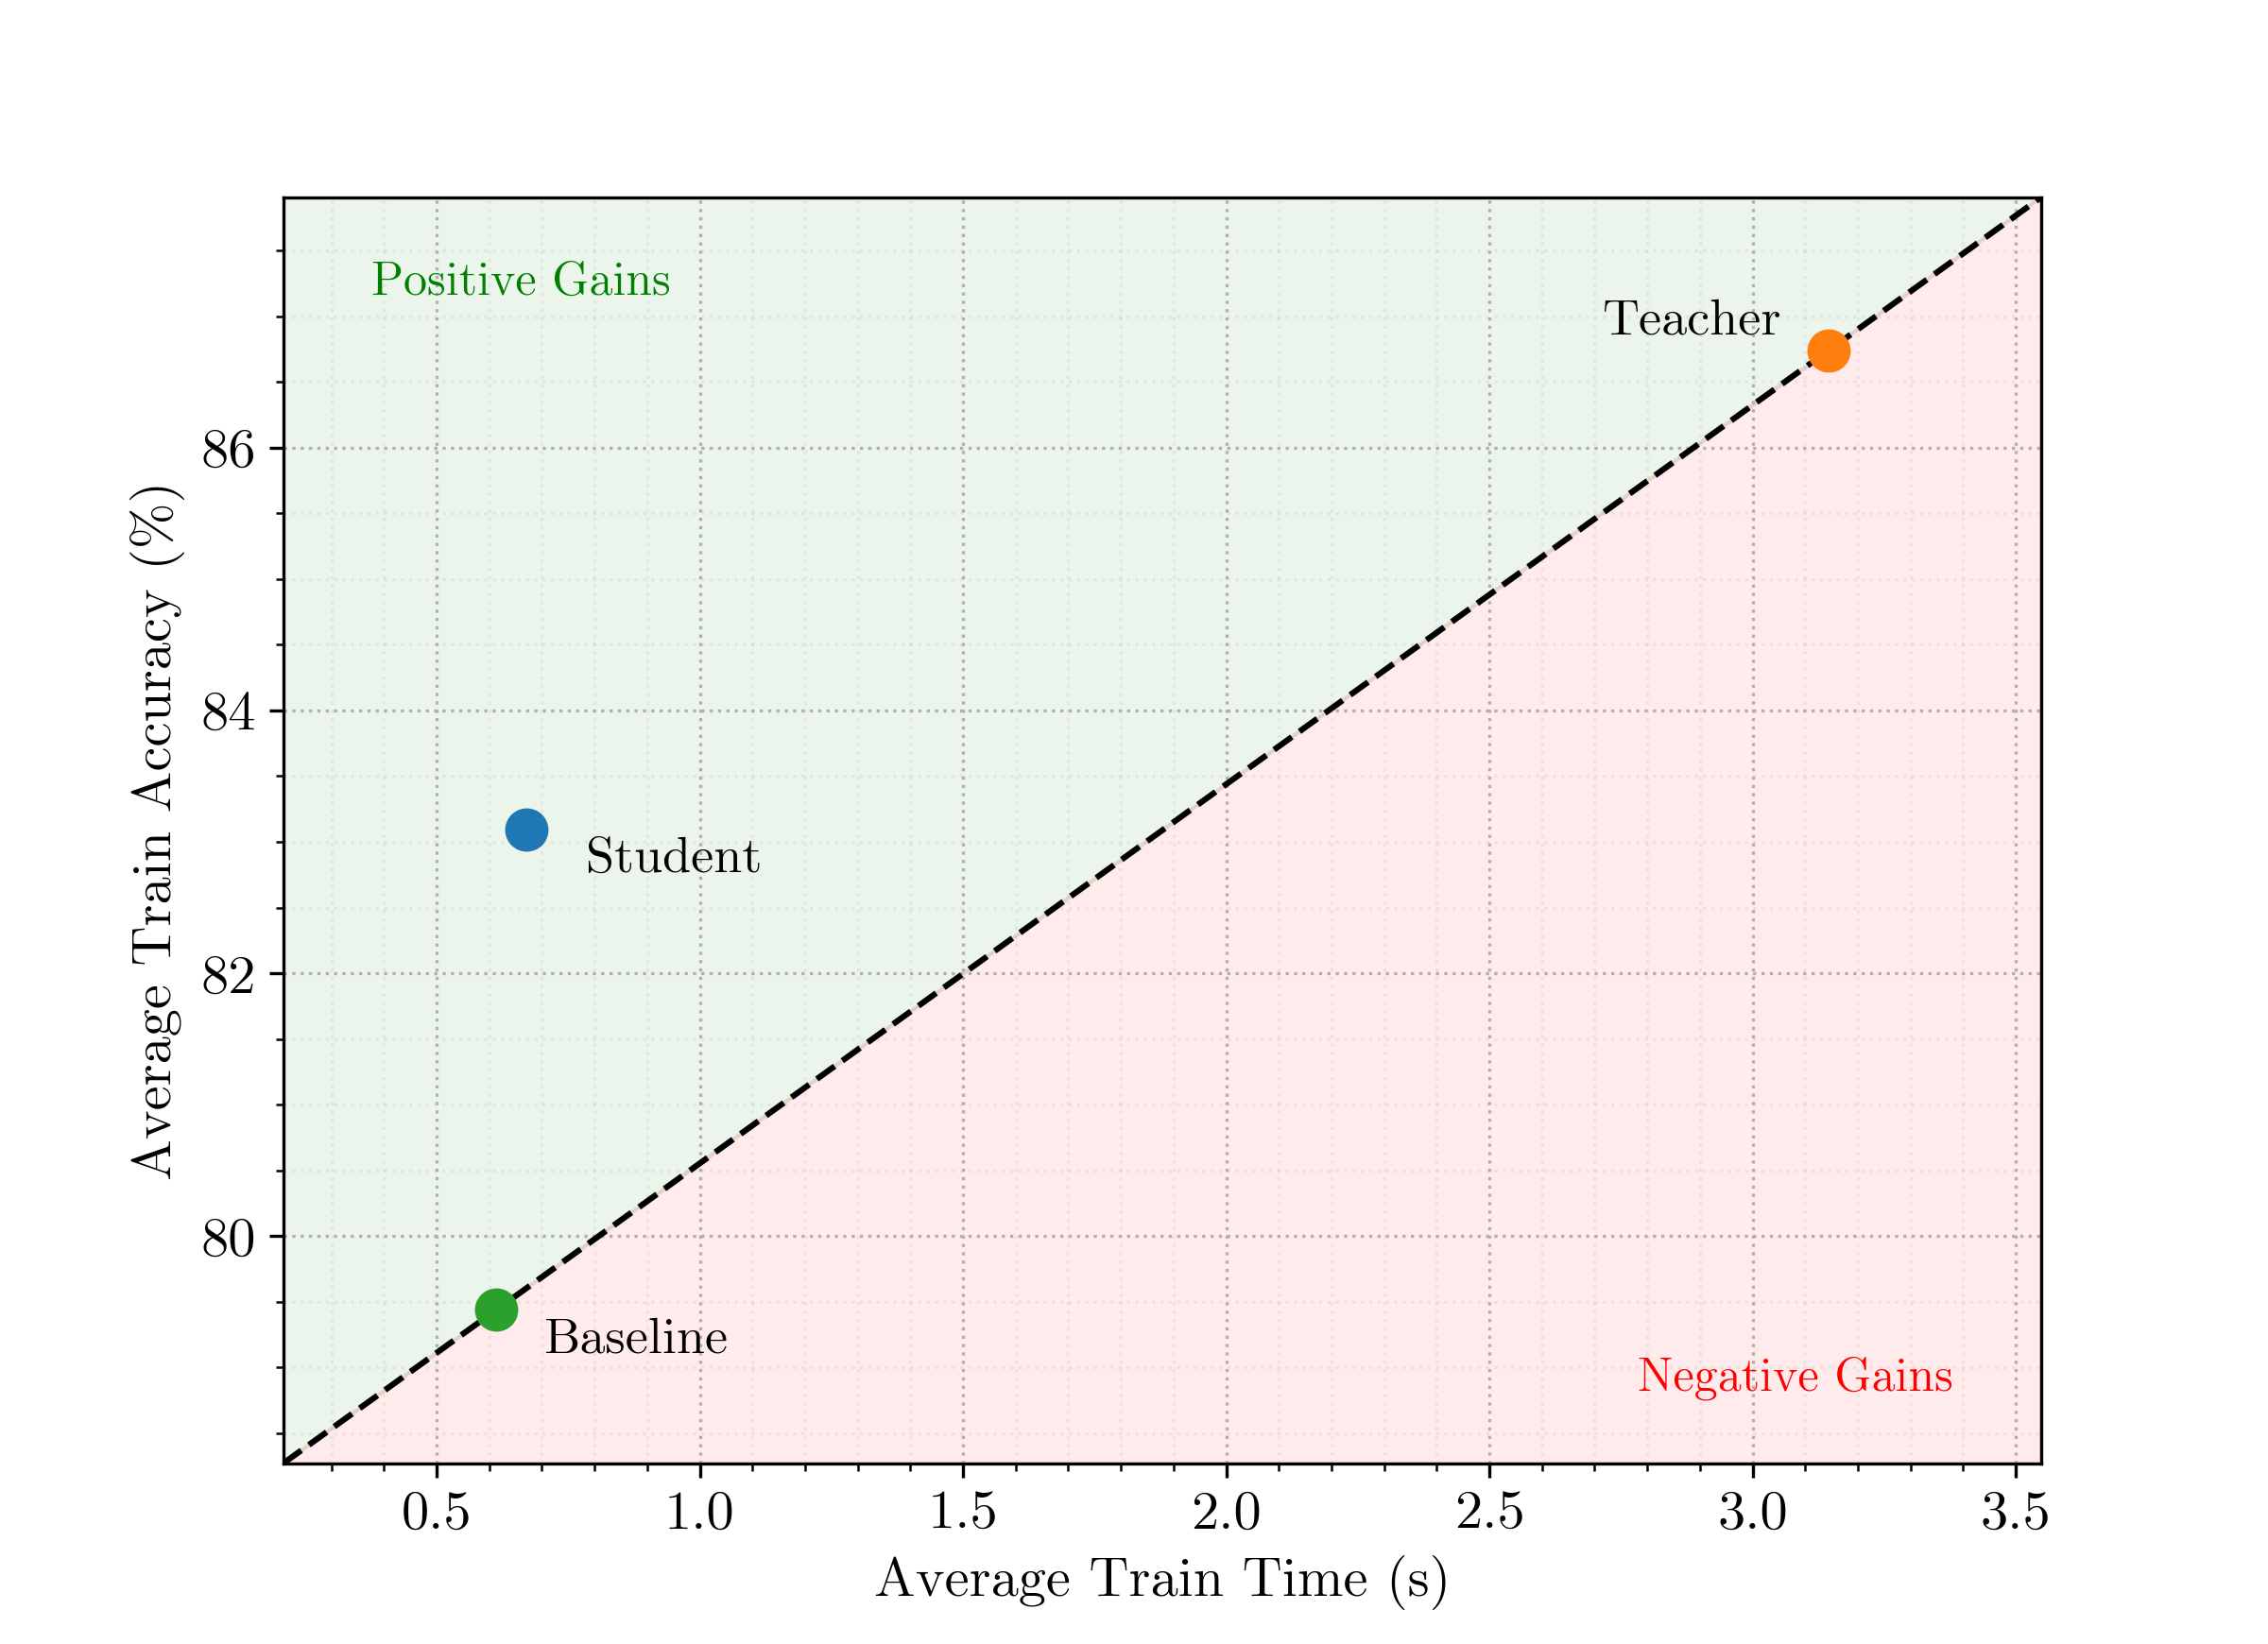
\includegraphics[width=\linewidth]{EMNIST_train_efficiency.png}
        \caption{Training efficiency on EMNIST using DKD.}
        \label{fig:train-eff-emnist}
    \end{subfigure}
    \caption{Training accuracy and efficiency on EMNIST using DKD.}
    \label{fig:train-emnist-combined}
\end{figure}

For MNIST, the distilled model $TM_D$ increases training accuracy over the student by approximately 5 percentage points, with reduced variance and slightly lower training time. On KMNIST, $TM_D$ achieves modest gains, increasing average accuracy by around 2 percentage points with similar epoch times. On the IMDB dataset, $TM_D$ achieves accuracy between the teacher and student while reducing training time by roughly half. This is enabled by rapid literal pruning guided by the teacher, and IMDB results stabilize more quickly than the MNIST datasets, allowing for fewer epochs.

The temporary drop in accuracy at $E = E_T$ in each plot reflects the distilled model's adjustment to clause transfer. The student model $TM_S$ is trained from scratch, whereas the distilled model $TM_D$ starts with $|C_S|$ clauses copied from $TM_T$ after $E_T$ epochs. The distilled model needs several epochs to re-balance clause contributions in the absence of the remaining teacher clauses. For example, in Figure~\ref{fig:train-acc-emnist}, it takes approximately 7 epochs for $TM_D$ to reach the equilibrium accuracy of the student, which is fewer epochs than required for the student to reach the same level. This demonstrates that clause initialization combined with distribution-enhanced fitting enables efficient training of a smaller model.

\subsection{Testing Accuracy and Performance Analysis}

The results on the test datasets further confirm that our teacher-student knowledge distillation framework improves both accuracy and performance. Table~\ref{tab:test-table-dkd} summarizes the testing performance of each model across all datasets.

Figure~\ref{fig:test-acc-combined} shows the average accuracy of each model for each dataset. As described in Table~\ref{tab:test-table-dkd}, each distilled model \DIFdelbegin \DIFdel{significantly }\DIFdelend \DIFaddbegin \DIFadd{consistently }\DIFaddend outperforms its respective baseline student model \DIFaddbegin \DIFadd{across the evaluated datasets}\DIFaddend . 

\begin{table*}
\centering
\caption{Testing Results (DKD)}
\begin{tabular}{|l|c|c|c|c|c|c|}
\hline
Dataset & $Acc_T$ & $\mathcal{T}_T$ & $Acc_S$ & $\mathcal{T}_S$ & $Acc_D$ & $\mathcal{T}_D$ \\
\hline
MNIST & 95.20 \newline $\pm$ 0.06 & 0.37 \newline $\pm$ 0.01 & 90.37 \newline $\pm$ 0.14 & 0.06 \newline $\pm$ 0.00 & 93.96 \newline $\pm$ 0.06 & 0.06 \newline $\pm$ 0.00 \\\hline%\hdashline
KMNIST & 85.37 \newline $\pm$ 0.10 & 0.97 \newline $\pm$ 0.01 & 80.11 \newline $\pm$ 0.10 & 0.10 \newline $\pm$ 0.00 & 82.48 \newline $\pm$ 0.07 & 0.10 \newline $\pm$ 0.00 \\\hline%\hdashline
EMNIST & 80.96 \newline $\pm$ 0.10 & 3.27 \newline $\pm$ 0.06 & 77.52 \newline $\pm$ 0.05 & 0.26 \newline $\pm$ 0.00 & 80.31 \newline $\pm$ 0.07 & 0.26 \newline $\pm$ 0.00 \\\hline%\hdashline
IMDB & 88.96 \newline $\pm$ 0.04 & 17.88 \newline $\pm$ 0.71 & 87.85 \newline $\pm$ 0.24 & 10.37 \newline $\pm$ 0.30 & 88.62 \newline $\pm$ 0.03 & 9.36 \newline $\pm$ 0.17 \\
\hline
\end{tabular}
\label{tab:test-table-dkd}
\end{table*}


\begin{figure}[h]
    \centering
    \begin{subfigure}[b]{0.49\linewidth}
        \centering
        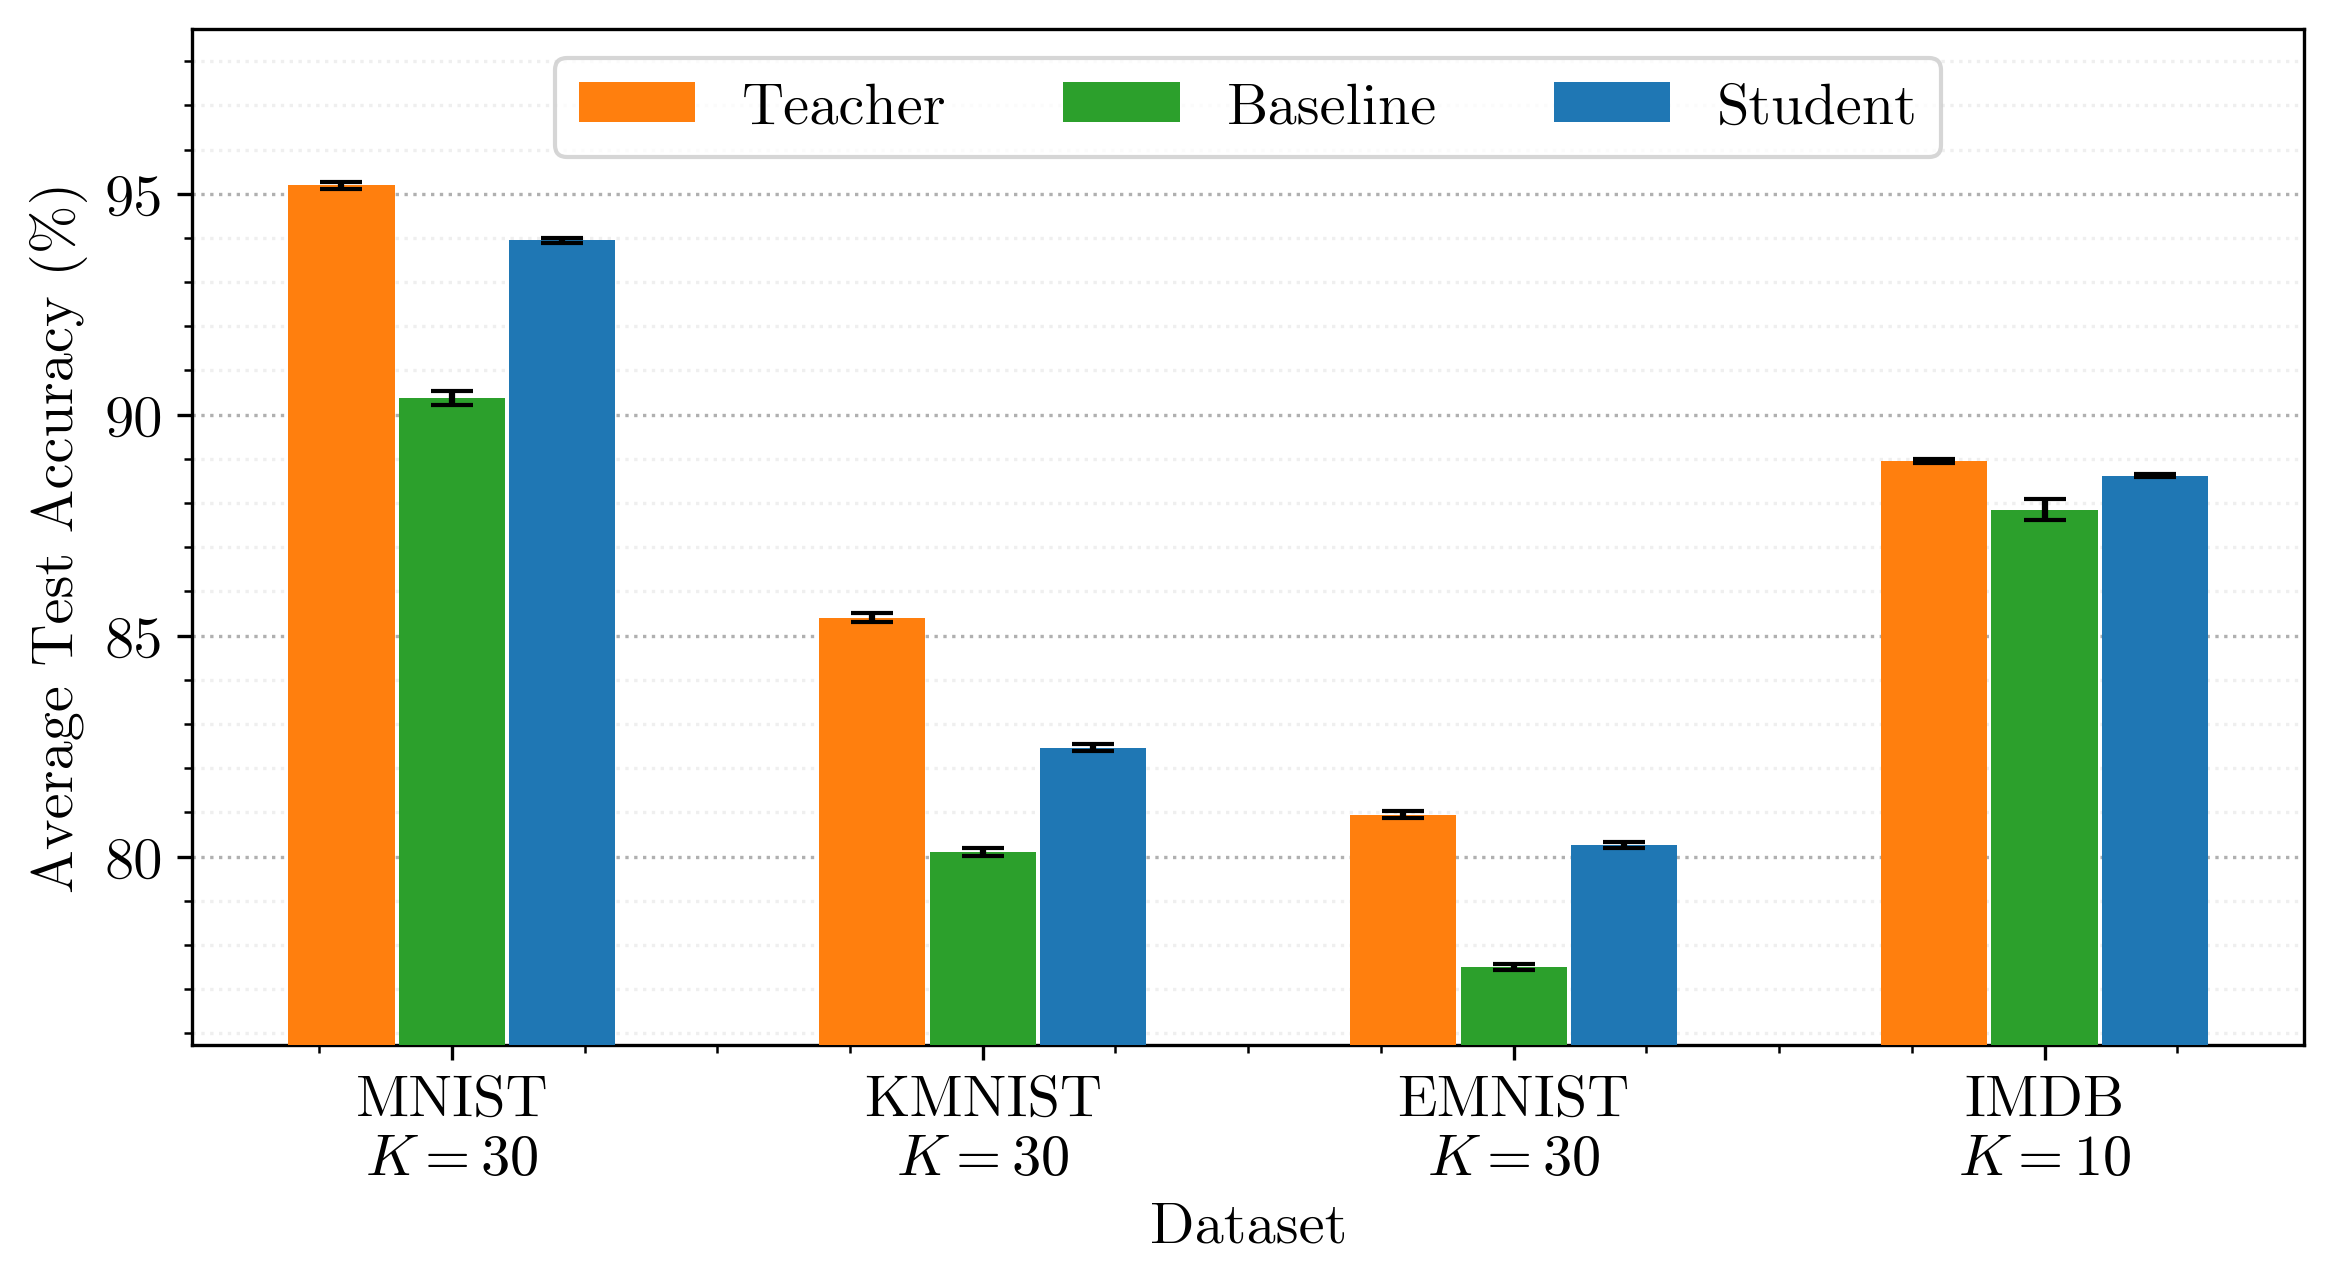
\includegraphics[width=\linewidth]{combined_test_acc.png}
        \caption{Average testing accuracy $Acc$ on each dataset using DKD.}
        \label{fig:test-acc-combined}
    \end{subfigure}
    \hfill
    \begin{subfigure}[b]{0.49\linewidth}
        \centering
        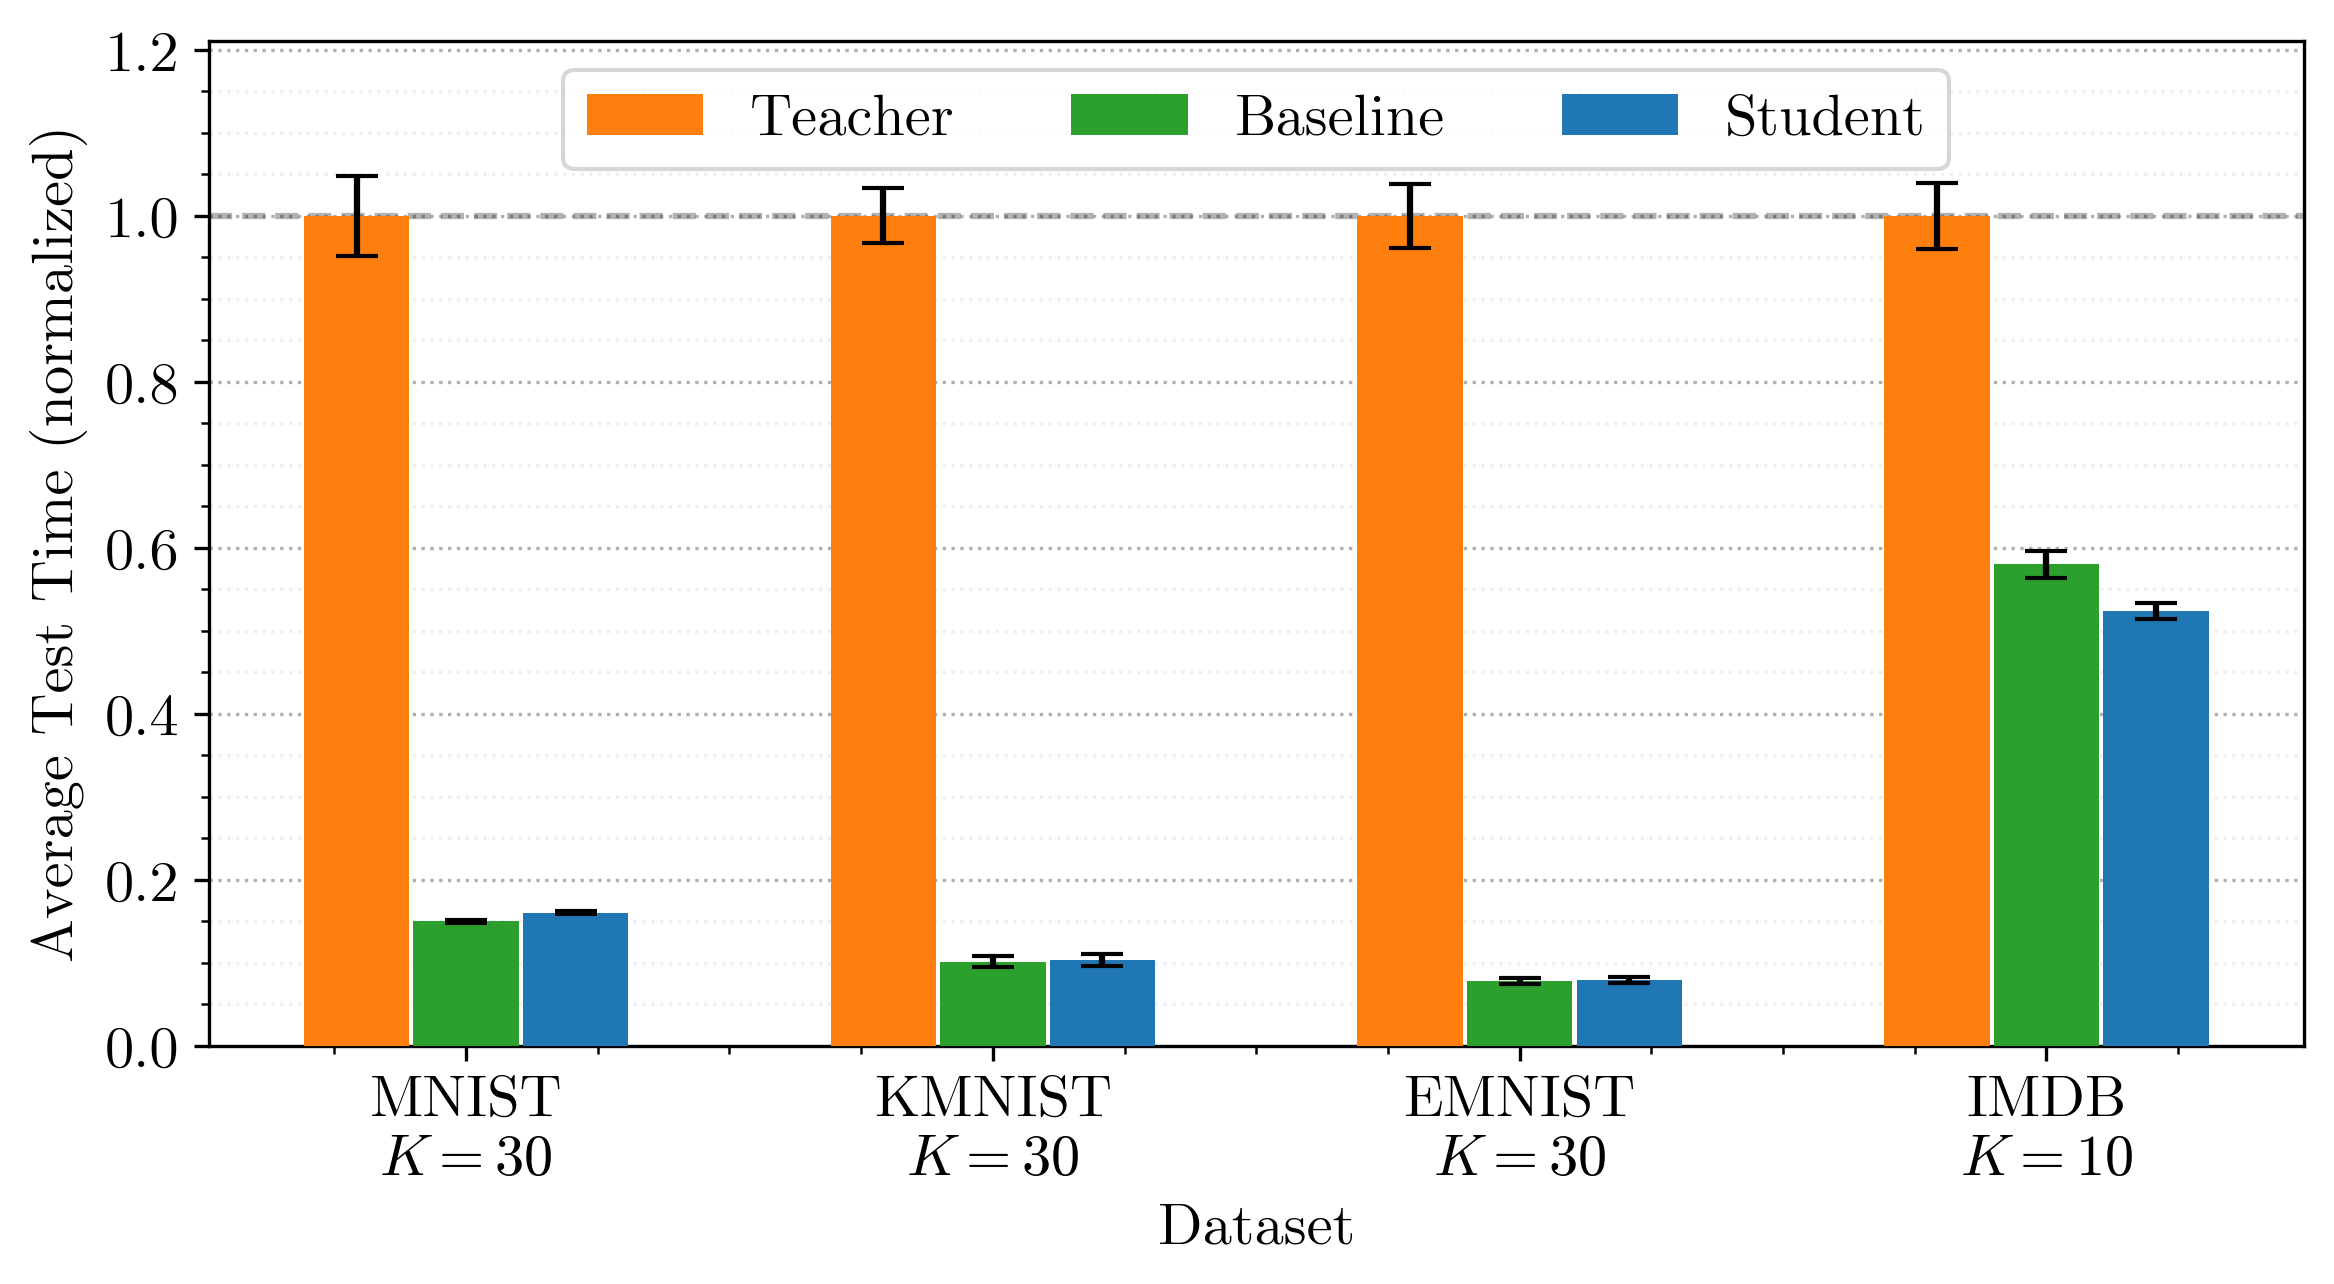
\includegraphics[width=\linewidth]{combined_test_time.png}
        \caption{Average testing epoch time $\mathcal{T}$ on each dataset using DKD.}
        \label{fig:test-time-combined}
    \end{subfigure}
    \caption{Testing accuracy and epoch time on each dataset using DKD.}
    \label{fig:test-acc-time-combined}
\end{figure}

Figure~\ref{fig:test-time-combined} shows the normalized average testing time per epoch relative to the teacher. Normalization allows a fair comparison across datasets of different sizes (see Table~\ref{tab:dataset-size}). We observe that each distilled model achieves testing performance similar to its respective baseline student model while improving accuracy.

For EMNIST, the distilled model demonstrates \DIFdelbegin \DIFdel{remarkable efficiency }\DIFdelend \DIFaddbegin \DIFadd{notable efficiency under the evaluated settings}\DIFaddend . As shown in Figure~\ref{fig:test-eff-emnist}, $TM_D$ achieves near-teacher accuracy while reducing inference time by roughly 12$\times$. The accuracy is comparable to multi-layer Tsetlin Machines reported in~\cite{gorbenko2024multi}, but with \DIFdelbegin \DIFdel{significantly }\DIFdelend lower inference time and \DIFdelbegin \DIFdel{memory usage }\DIFdelend \DIFaddbegin \DIFadd{a reduced number of clauses }\DIFaddend (Figures~\ref{fig:test-acc-emnist} and~\ref{fig:test-time-combined}). \DIFaddbegin \DIFadd{While clause count is a primary determinant of memory usage in Tsetlin Machines, explicit memory footprint measurements are not reported in this study.
}\DIFaddend 

\begin{figure}[h]
    \centering
    \begin{subfigure}[b]{0.49\linewidth}
        \centering
        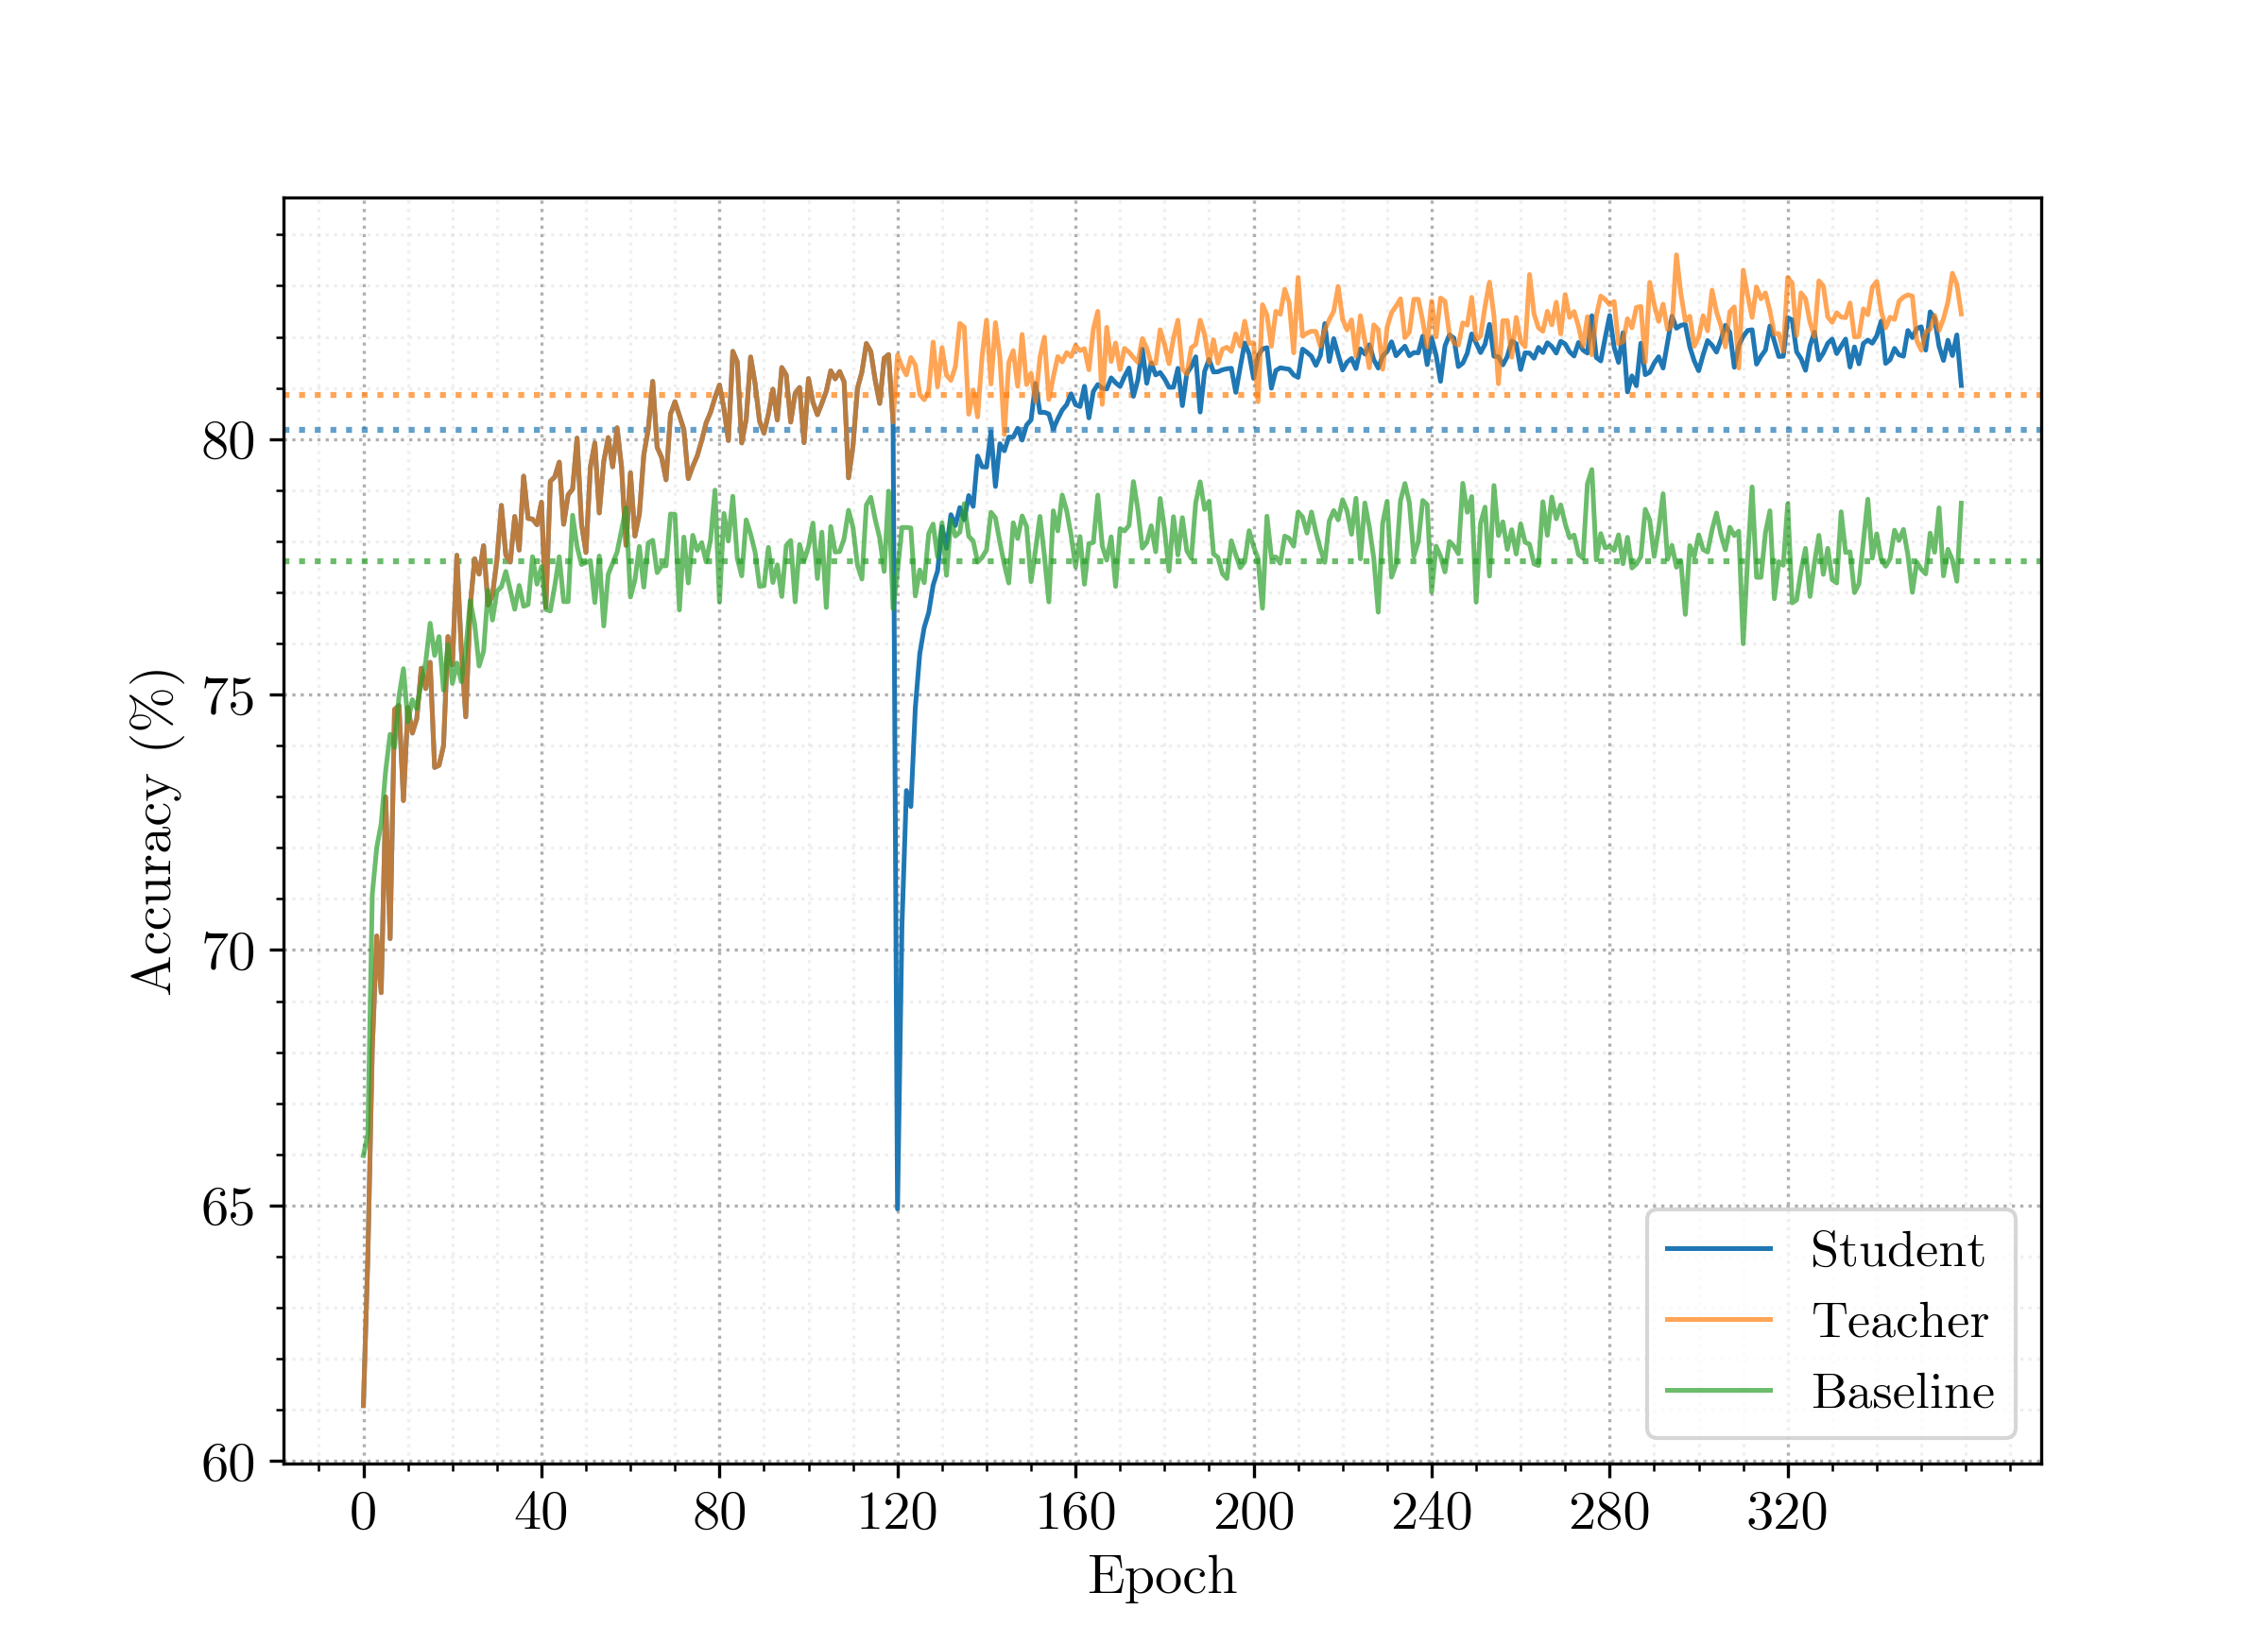
\includegraphics[width=\linewidth]{EMNIST_test_accuracy.png}
        \caption{Testing accuracy $Acc$ on EMNIST using DKD.}
        \label{fig:test-acc-emnist}
    \end{subfigure}
    \hfill
    \begin{subfigure}[b]{0.49\linewidth}
        \centering
        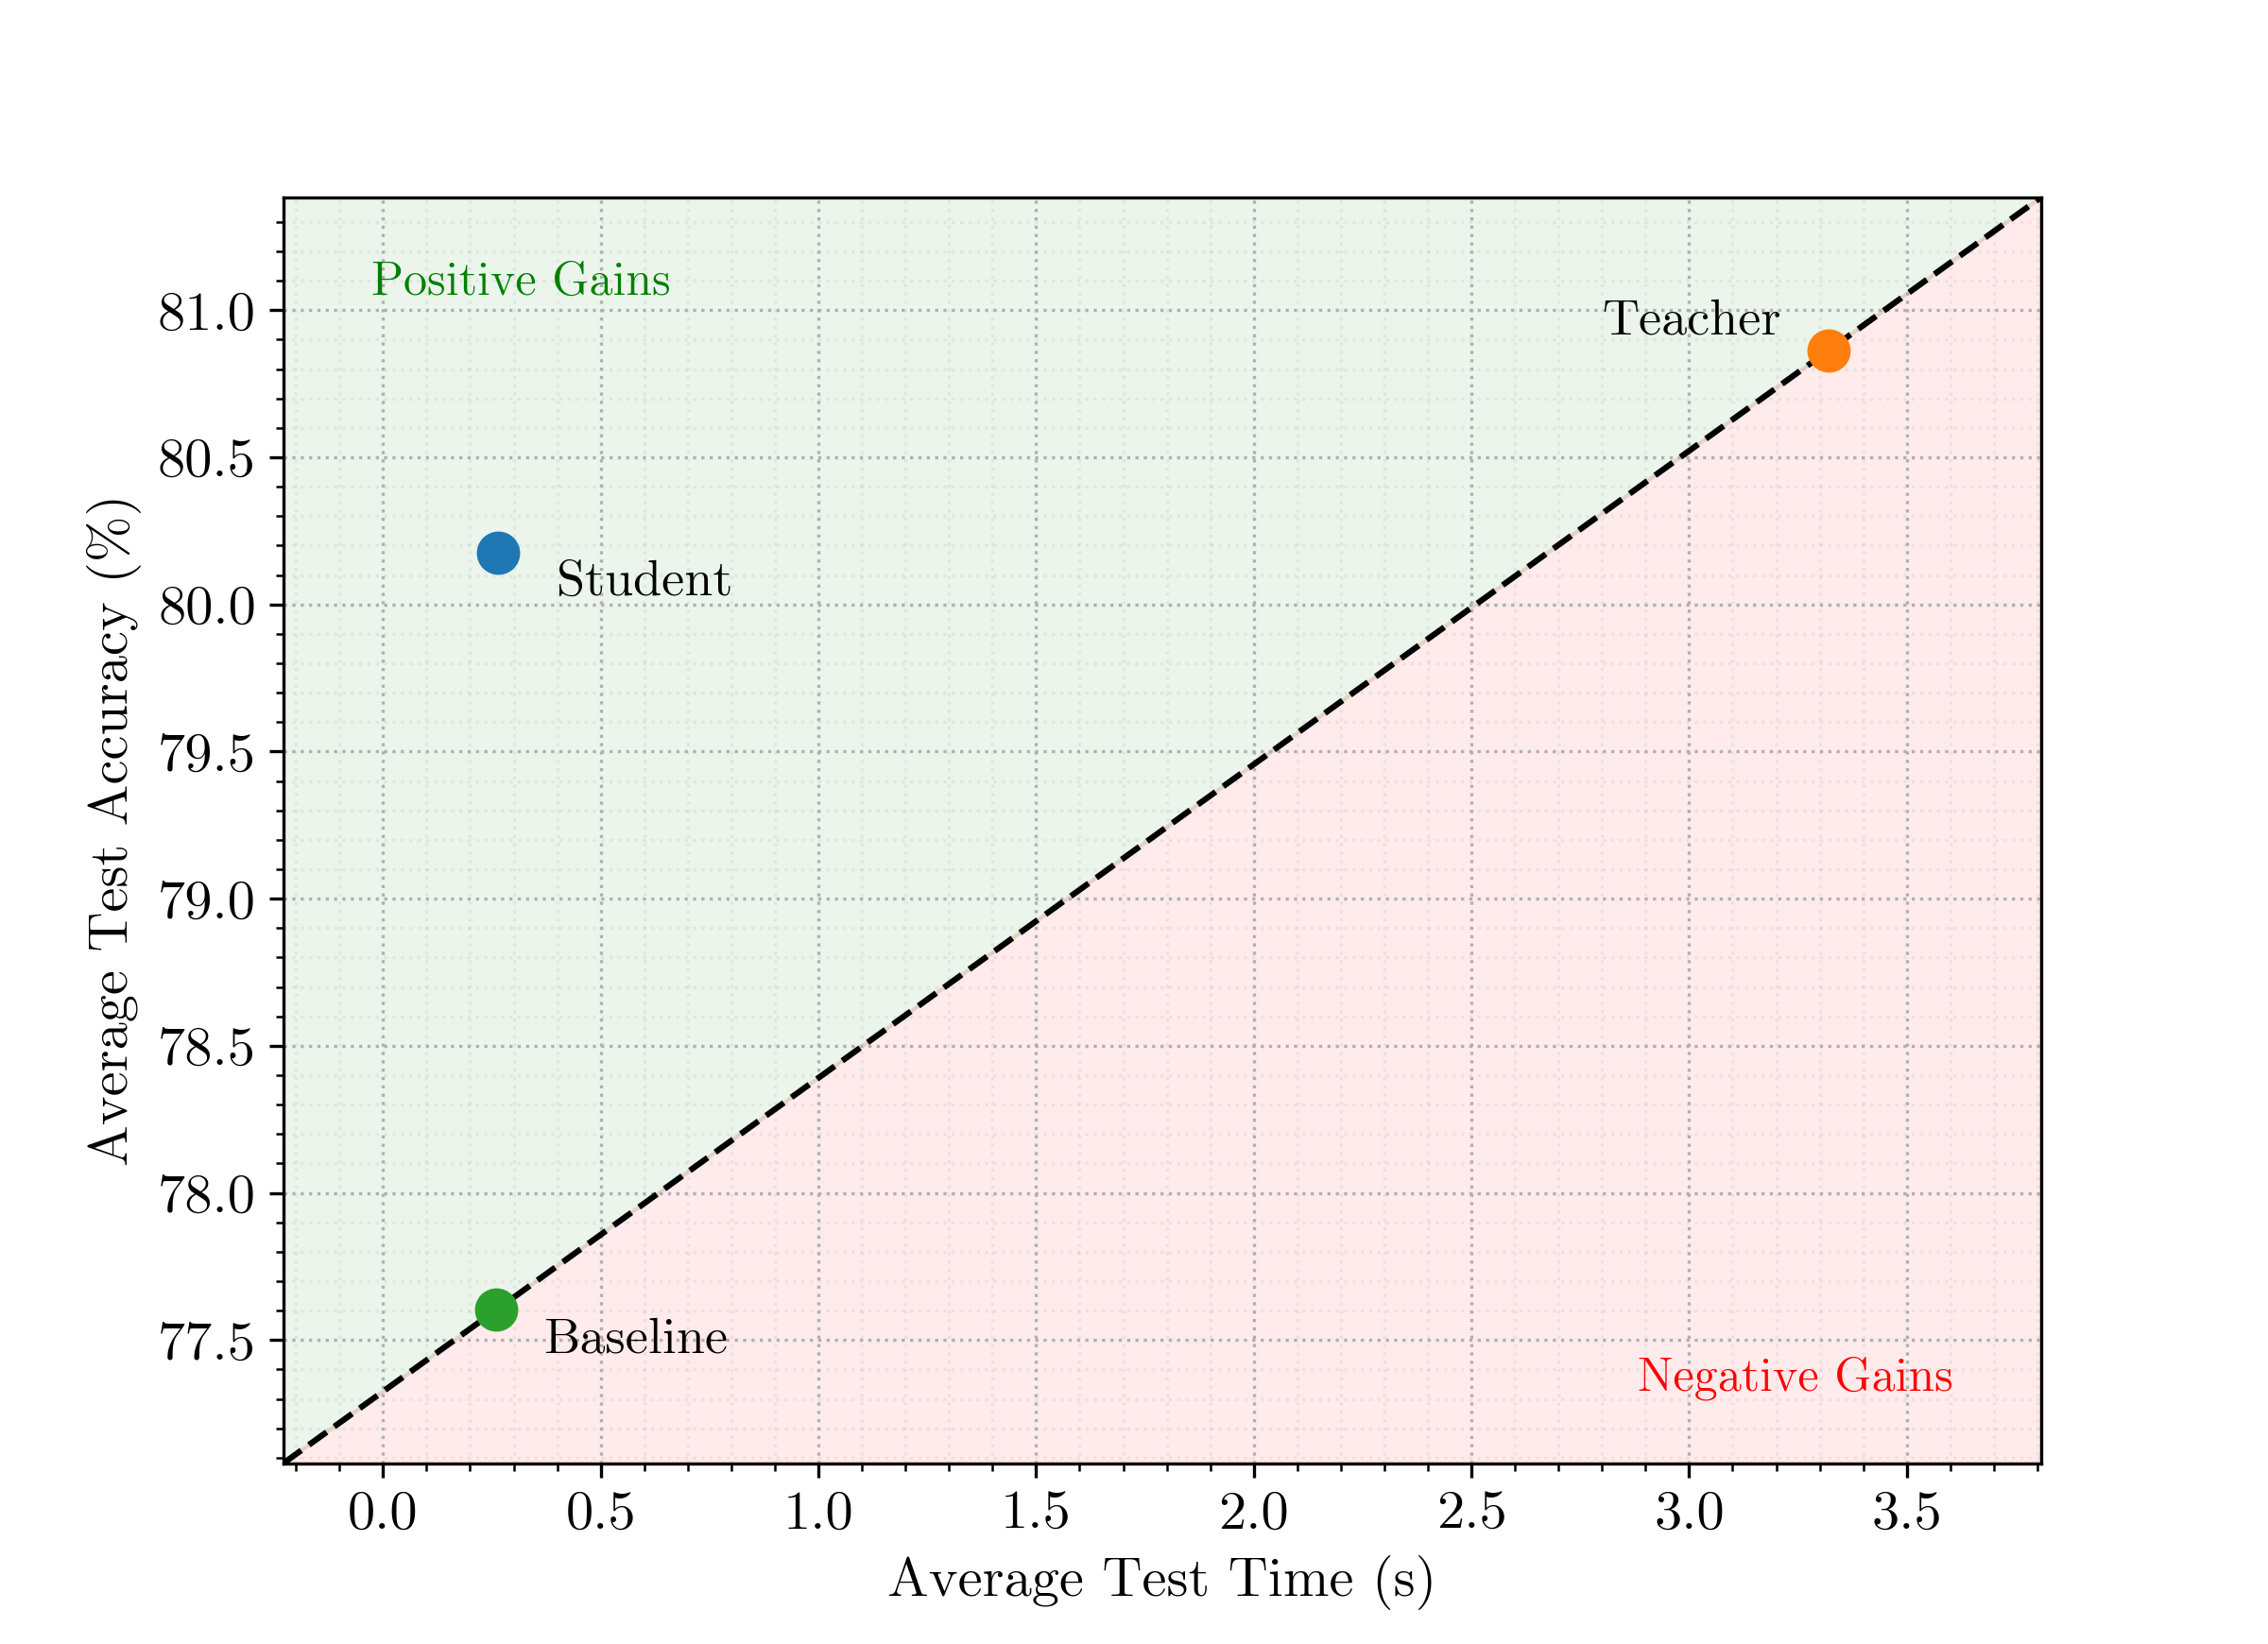
\includegraphics[width=\linewidth]{EMNIST_test_efficiency.png}
        \caption{Testing efficiency on EMNIST using DKD.}
        \label{fig:test-eff-emnist}
    \end{subfigure}
    \caption{Testing accuracy and efficiency on EMNIST \DIFdelbeginFL \DIFdelFL{using DKD.}\DIFdelendFL \DIFaddbeginFL \DIFaddFL{for teacher, student, and distilled models}\DIFaddendFL }
    \label{fig:test-emnist-combined}
\end{figure}

MNIST testing results reflect similar trends: $TM_D$ improves accuracy over the student by approximately 3.5--5 percentage points while maintaining or slightly reducing testing time. On KMNIST, the distilled model exceeds the student baseline by about 2.5 percentage points without increasing execution time. For IMDB, $TM_D$ improves accuracy by roughly 1 percentage point while decreasing inference time compared to both student and teacher models.

The temporary drop in accuracy at $E_T$ epochs is also observed in testing, for the same reasons described in Section~\ref{sec:trapa}.

\subsection{Activation Analysis}

The influence of the teacher on the student can be visualized through activation maps generated over the input data. Figure~\ref{fig:activation-emnist} shows an example on EMNIST test samples. For each pixel, green indicates an included positive feature (e.g., a white pixel), and red indicates an included negated feature (e.g., a black pixel). Pixel intensity reflects feature importance.

Teacher activation maps are denser than those of the student, as expected given the student has 10$\times$ fewer clauses. The distilled model, with the same number of clauses as the teacher, exhibits a slightly wider range of included features, leveraging the additional context provided by clause transfer. This contributes to the improved accuracy of the distilled model \footnote{Activation maps are straightforward to generate for image datasets but are less interpretable for textual datasets such as IMDB.}. 

Even with identical model sizes, $TM_D$ shows lower activation entropy (3.1 vs 3.6), indicating more focused and strategic feature usage, which \DIFdelbegin \DIFdel{explains its superior }\DIFdelend \DIFaddbegin \DIFadd{provides insight into its improved }\DIFaddend accuracy. Note that these visualizations are limited to image datasets; text feature patterns are less spatially interpretable.

\DIFdelbegin %DIFDELCMD < \begin{figure}[H]
%DIFDELCMD <     %%%
\DIFdelendFL \DIFaddbeginFL \begin{figure}[h]
    \DIFaddendFL \centering
    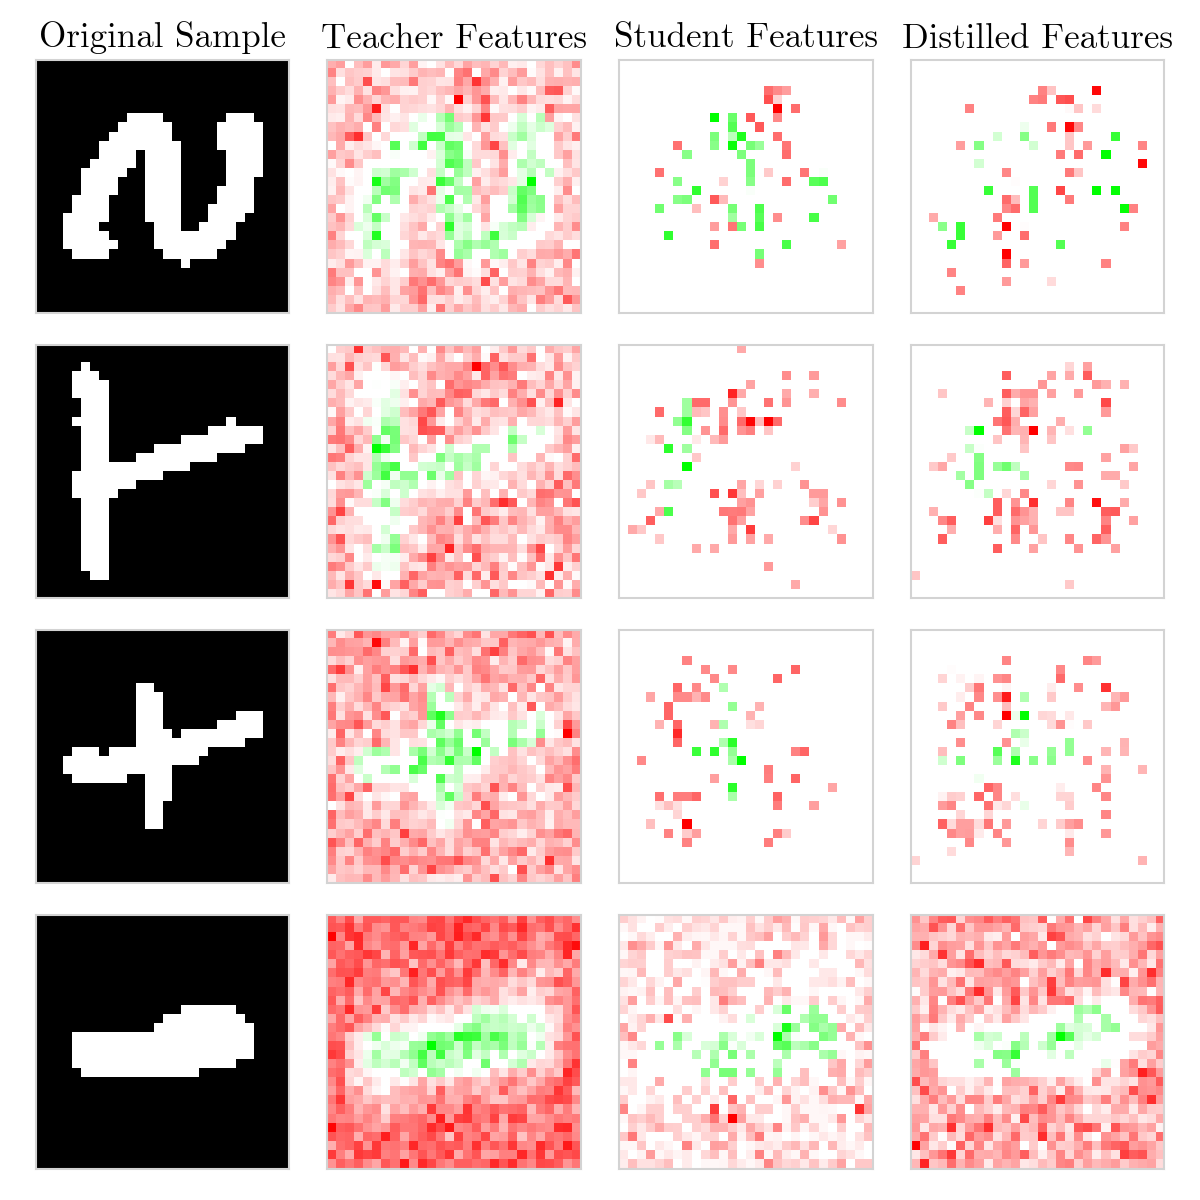
\includegraphics[width=0.8\linewidth]{EMNIST_activation_maps.png}
    \caption{Activation maps for $TM_T$, $TM_S$, and $TM_D$ on four EMNIST test samples.}
    \label{fig:activation-emnist}
\end{figure}

 %DIF <  \section{Conclusion}
%DIF <  This paper puts forward a novel framework for implementing knowledge distillation in Tsetlin Machines. It introduces a hybrid feature- and response-based method to distill information from a larger teacher model to a smaller student model. Our results have shown that a small distilled model can significantly outperform a parametrically identical model at the same size, increasing accuracy without increasing latency. This has consequential results in the relatively new domain of Tsetlin Machines. Notably, knowledge distillation was achieved without any sort of loss function, which is a key component in traditional, neural-network-based distillation. The exclusion of a loss function preserves the ability of Tsetlin Machines to run on low power, edge computing devices where complex math operations are prohibited or computationally expensive. 
\DIFaddbegin \section{\DIFadd{Limitations}}
 \DIFadd{While our Distribution-Enhanced Knowledge Distillation demonstrates consistent empirical improvements, several limitations warrant acknowledgment.
}\DIFaddend 

\DIFdelbegin \section{\DIFdel{Discussion and Conclusion}}
%DIFAUXCMD
\addtocounter{section}{-1}%DIFAUXCMD
\DIFdelend \DIFaddbegin \DIFadd{Our experiments focus on relatively simple, balanced datasets with moderate feature dimensionality (784--5000 features). Performance on high-dimensional problems, severely imbalanced classes, or complex domains (e.g., medical imaging, time-series) remains unexplored. Notably, IMDB shows a modest improvement of 0.57 percentage points, suggesting that distillation effectiveness may vary across domains.
}\DIFaddend 

\DIFaddbegin \DIFadd{We do not compare against simpler compression alternatives such as direct clause pruning from the teacher or training the student model for $E_{T+S}$ total epochs. Additionally, explicit memory consumption measurements and actual edge device deployment tests are not included in this study and would be required to fully substantiate practical applicability claims.
}

\DIFadd{Our approach lacks formal analysis of approximation bounds or information-theoretic characterization of what ``dark knowledge'' the soft labels capture in propositional logic systems. Understanding why temperature values $\tau \in [3.0, 4.0]$ work well for TMs, compared to $\tau \approx 1$--2 typical in neural networks, requires further investigation.
}

\DIFadd{Further research could be directed at optimizing the balance $\alpha$, weight transfer $z$, and temperature $\tau$ parameters, through automated hyperparameter search methods, or exploring adaptive temperature scheduling during training similar to curriculum learning approaches. Investigating whether temperature should vary by dataset characteristics (e.g., number of classes, class imbalance) could yield additional insights. The clause transfer algorithm could also be improved by considering clause coverage on all features, not just diversity and weight. Instead of solely using offline distillation as shown in this paper, further research could also be directed at comparing the effects of online and offline distillation. We would also explore the application of our algorithm in other domains like few-shot learning \mbox{%DIFAUXCMD
\cite{anjum2025using, DBLP:conf/bigdataconf/GuoAZ22, anjum2025weighted} }\hskip0pt%DIFAUXCMD
and bioinformatics \mbox{%DIFAUXCMD
\cite{woessner2024identifying}}\hskip0pt%DIFAUXCMD
, where data is few and knowledge transfer can help training these models with limited data.
}



\section{\DIFadd{Conclusion}}
%DIF >  This paper puts forward a novel framework for implementing knowledge distillation in Tsetlin Machines. It introduces a hybrid feature- and response-based method to distill information from a larger teacher model to a smaller student model. Our results have shown that a small distilled model can significantly outperform a parametrically identical model at the same size, increasing accuracy without increasing latency. This has consequential results in the relatively new domain of Tsetlin Machines. Notably, knowledge distillation was achieved without any sort of loss function, which is a key component in traditional, neural-network-based distillation. The exclusion of a loss function preserves the ability of Tsetlin Machines to run on low power, edge computing devices where complex math operations are prohibited or computationally expensive. 

\DIFaddend Clause-based knowledge distillation substantially accelerates Tsetlin Machine training while preserving or improving accuracy. Distilled models \DIFdelbegin \DIFdel{reach performance close to, or in some cases surpass, the teacher }\DIFdelend \DIFaddbegin \DIFadd{approach or occasionally exceed teacher performance under specific settings}\DIFaddend , particularly for IMDB and MNIST3D datasets. The method is especially effective when feature counts $|L_T|$ and $|L_S|$ exceed total teacher clauses $|C_T| \times |\zeta|$, highlighting the importance of clause density.

Activation map analysis confirms that the distilled model leverages teacher clause context to strategically select features. Training and inference times are \DIFdelbegin \DIFdel{significantly }\DIFdelend reduced, demonstrating practical efficiency\DIFdelbegin \DIFdel{.
}%DIFDELCMD < 

%DIFDELCMD < %%%
\subsection{\DIFdel{Limitations}}
%DIFAUXCMD
\addtocounter{subsection}{-1}%DIFAUXCMD
%DIFDELCMD < 

%DIFDELCMD < %%%
\DIFdel{DKD was tested on moderate-dimensional, relatively balanced datasets. Its performance on high-dimensional, highly imbalanced, or more complex domains remains unexplored. Gains on IMDB were modest (0.57pp), indicating domain-dependent effectiveness. We do not compare directly with simpler compression strategies or evaluate memory usage and edge-device deployment. Formal analysis of soft-label information in propositional logic systems remains future work. Adaptive temperature scheduling, online vs. offline distillation, and refined clause transfer methods are promising avenues for further exploration.
}%DIFDELCMD < 

%DIFDELCMD < %%%
\subsection{\DIFdel{Future Work}}
%DIFAUXCMD
\addtocounter{subsection}{-1}%DIFAUXCMD
%DIFDELCMD < 

%DIFDELCMD < %%%
\DIFdel{Future directions include investigating teacher and student hyperparameter effects, automated hyperparameter optimization, dataset-specific temperature scheduling, online/offline distillation comparisons, and application to low-data domains such as few-shot learning \mbox{%DIFAUXCMD
\cite{anjum2025using, DBLP:conf/bigdataconf/GuoAZ22, anjum2025weighted} }\hskip0pt%DIFAUXCMD
and bioinformatics \mbox{%DIFAUXCMD
\cite{woessner2024identifying}}\hskip0pt%DIFAUXCMD
}\DIFdelend .


During the preparation of this work the author(s) used Claude and ChatGPT in order to fix grammatical and syntax errors and clarify the material in the paper. After using this tool/service, the author(s) reviewed and edited the content as needed and take(s) full responsibility for the content of the published article.

% \begin{appendices}

% \input{appendix}

%%=============================================%%
%% For submissions to Nature Portfolio Journals %%
%% please use the heading ``Extended Data''.   %%
%%=============================================%%

%%=============================================================%%
%% Sample for another appendix section			       %%
%%=============================================================%%

%% \section{Example of another appendix section}\label{secA2}%
%% Appendices may be used for helpful, supporting or essential material that would otherwise 
%% clutter, break up or be distracting to the text. Appendices can consist of sections, figures, 
%% tables and equations etc.

%%===========================================================================================%%
%% If you are submitting to one of the Nature Portfolio journals, using the eJP submission   %%
%% system, please include the references within the manuscript file itself. You may do this  %%
%% by copying the reference list from your .bbl file, paste it into the main manuscript .tex %%
%% file, and delete the associated \verb+\bibliography+ commands.                            %%
%%===========================================================================================%%


%% BioMed_Central_Bib_Style_v1.01

\begin{thebibliography}{47}
% BibTex style file: bmc-mathphys.bst (version 2.1), 2014-07-24
\ifx \bisbn   \undefined \def \bisbn  #1{ISBN #1}\fi
\ifx \binits  \undefined \def \binits#1{#1}\fi
\ifx \bauthor  \undefined \def \bauthor#1{#1}\fi
\ifx \batitle  \undefined \def \batitle#1{#1}\fi
\ifx \bjtitle  \undefined \def \bjtitle#1{#1}\fi
\ifx \bvolume  \undefined \def \bvolume#1{\textbf{#1}}\fi
\ifx \byear  \undefined \def \byear#1{#1}\fi
\ifx \bissue  \undefined \def \bissue#1{#1}\fi
\ifx \bfpage  \undefined \def \bfpage#1{#1}\fi
\ifx \blpage  \undefined \def \blpage #1{#1}\fi
\ifx \burl  \undefined \def \burl#1{\textsf{#1}}\fi
\ifx \doiurl  \undefined \def \doiurl#1{\url{https://doi.org/#1}}\fi
\ifx \betal  \undefined \def \betal{\textit{et al.}}\fi
\ifx \binstitute  \undefined \def \binstitute#1{#1}\fi
\ifx \binstitutionaled  \undefined \def \binstitutionaled#1{#1}\fi
\ifx \bctitle  \undefined \def \bctitle#1{#1}\fi
\ifx \beditor  \undefined \def \beditor#1{#1}\fi
\ifx \bpublisher  \undefined \def \bpublisher#1{#1}\fi
\ifx \bbtitle  \undefined \def \bbtitle#1{#1}\fi
\ifx \bedition  \undefined \def \bedition#1{#1}\fi
\ifx \bseriesno  \undefined \def \bseriesno#1{#1}\fi
\ifx \blocation  \undefined \def \blocation#1{#1}\fi
\ifx \bsertitle  \undefined \def \bsertitle#1{#1}\fi
\ifx \bsnm \undefined \def \bsnm#1{#1}\fi
\ifx \bsuffix \undefined \def \bsuffix#1{#1}\fi
\ifx \bparticle \undefined \def \bparticle#1{#1}\fi
\ifx \barticle \undefined \def \barticle#1{#1}\fi
\bibcommenthead
\ifx \bconfdate \undefined \def \bconfdate #1{#1}\fi
\ifx \botherref \undefined \def \botherref #1{#1}\fi
\ifx \url \undefined \def \url#1{\textsf{#1}}\fi
\ifx \bchapter \undefined \def \bchapter#1{#1}\fi
\ifx \bbook \undefined \def \bbook#1{#1}\fi
\ifx \bcomment \undefined \def \bcomment#1{#1}\fi
\ifx \oauthor \undefined \def \oauthor#1{#1}\fi
\ifx \citeauthoryear \undefined \def \citeauthoryear#1{#1}\fi
\ifx \endbibitem  \undefined \def \endbibitem {}\fi
\ifx \bconflocation  \undefined \def \bconflocation#1{#1}\fi
\ifx \arxivurl  \undefined \def \arxivurl#1{\textsf{#1}}\fi
\csname PreBibitemsHook\endcsname

%%% 1
\bibitem[\protect\citeauthoryear{Hinton
  et~al.}{2015}]{hinton2015distillingknowledgeneuralnetwork}
\begin{botherref}
\oauthor{\bsnm{Hinton}, \binits{G.}},
\oauthor{\bsnm{Vinyals}, \binits{O.}},
\oauthor{\bsnm{Dean}, \binits{J.}}:
Distilling the Knowledge in a Neural Network
(2015).
\url{https://arxiv.org/abs/1503.02531}
\end{botherref}
\endbibitem

%%% 2
\bibitem[\protect\citeauthoryear{DeepSeek-AI
  et~al.}{2025}]{deepseekai2025deepseekr1incentivizingreasoningcapability}
\begin{botherref}
\oauthor{\bsnm{DeepSeek-AI}}, et al.:
DeepSeek-R1: Incentivizing Reasoning Capability in LLMs via Reinforcement
  Learning
(2025).
\url{https://arxiv.org/abs/2501.12948}
\end{botherref}
\endbibitem

%%% 3
\bibitem[\protect\citeauthoryear{Matsuyama
  et~al.}{2025}]{matsuyama2025adaptive}
\begin{botherref}
\oauthor{\bsnm{Matsuyama}, \binits{K.}},
\oauthor{\bsnm{Anjum}, \binits{U.}},
\oauthor{\bsnm{Matsuyama}, \binits{S.}},
\oauthor{\bsnm{Shoda}, \binits{T.}},
\oauthor{\bsnm{Zhan}, \binits{J.}}:
Adaptive temperature based on logits correlation in knowledge distillation.
arXiv preprint arXiv:2503.09030
(2025)
\end{botherref}
\endbibitem

%%% 4
\bibitem[\protect\citeauthoryear{Granmo}{2018}]{granmo2018tsetlin}
\begin{botherref}
\oauthor{\bsnm{Granmo}, \binits{O.-C.}}:
The tsetlin machine--a game theoretic bandit driven approach to optimal pattern
  recognition with propositional logic.
arXiv preprint arXiv:1804.01508
(2018)
\end{botherref}
\endbibitem

%%% 5
\bibitem[\protect\citeauthoryear{Abeyrathna
  et~al.}{2021}]{abeyrathna2021massively}
\begin{bchapter}
\bauthor{\bsnm{Abeyrathna}, \binits{K.D.}},
\bauthor{\bsnm{Bhattarai}, \binits{B.}},
\bauthor{\bsnm{Goodwin}, \binits{M.}},
\bauthor{\bsnm{Gorji}, \binits{S.R.}},
\bauthor{\bsnm{Granmo}, \binits{O.-C.}},
\bauthor{\bsnm{Jiao}, \binits{L.}},
\bauthor{\bsnm{Saha}, \binits{R.}},
\bauthor{\bsnm{Yadav}, \binits{R.K.}}:
\bctitle{Massively parallel and asynchronous tsetlin machine architecture
  supporting almost constant-time scaling}.
In: \bbtitle{International Conference on Machine Learning},
pp. \bfpage{10}--\blpage{20}
(\byear{2021}).
\bcomment{PMLR}
\end{bchapter}
\endbibitem

%%% 6
\bibitem[\protect\citeauthoryear{Lei et~al.}{2020}]{lei2020arithmetic}
\begin{bchapter}
\bauthor{\bsnm{Lei}, \binits{J.}},
\bauthor{\bsnm{Wheeldon}, \binits{A.}},
\bauthor{\bsnm{Shafik}, \binits{R.}},
\bauthor{\bsnm{Yakovlev}, \binits{A.}},
\bauthor{\bsnm{Granmo}, \binits{O.-C.}}:
\bctitle{From arithmetic to logic based ai: A comparative analysis of neural
  networks and tsetlin machine}.
In: \bbtitle{2020 27th IEEE International Conference on Electronics, Circuits
  and Systems (ICECS)},
pp. \bfpage{1}--\blpage{4}
(\byear{2020}).
\bcomment{IEEE}
\end{bchapter}
\endbibitem

%%% 7
\bibitem[\protect\citeauthoryear{Xu et~al.}{2019}]{xu2019explainable}
\begin{bchapter}
\bauthor{\bsnm{Xu}, \binits{F.}},
\bauthor{\bsnm{Uszkoreit}, \binits{H.}},
\bauthor{\bsnm{Du}, \binits{Y.}},
\bauthor{\bsnm{Fan}, \binits{W.}},
\bauthor{\bsnm{Zhao}, \binits{D.}},
\bauthor{\bsnm{Zhu}, \binits{J.}}:
\bctitle{Explainable ai: A brief survey on history, research areas, approaches
  and challenges}.
In: \bbtitle{Natural Language Processing and Chinese Computing: 8th cCF
  International Conference, NLPCC 2019, Dunhuang, China, October 9--14, 2019,
  Proceedings, Part II 8},
pp. \bfpage{563}--\blpage{574}
(\byear{2019}).
\bcomment{Springer}
\end{bchapter}
\endbibitem

%%% 8
\bibitem[\protect\citeauthoryear{Do{\v{s}}ilovi{\'c}
  et~al.}{2018}]{dovsilovic2018explainable}
\begin{bchapter}
\bauthor{\bsnm{Do{\v{s}}ilovi{\'c}}, \binits{F.K.}},
\bauthor{\bsnm{Br{\v{c}}i{\'c}}, \binits{M.}},
\bauthor{\bsnm{Hlupi{\'c}}, \binits{N.}}:
\bctitle{Explainable artificial intelligence: A survey}.
In: \bbtitle{2018 41st International Convention on Information and
  Communication Technology, Electronics and Microelectronics (MIPRO)},
pp. \bfpage{0210}--\blpage{0215}
(\byear{2018}).
\bcomment{IEEE}
\end{bchapter}
\endbibitem

%%% 9
\bibitem[\protect\citeauthoryear{Anjum et~al.}{2022}]{anjum2022localization}
\begin{barticle}
\bauthor{\bsnm{Anjum}, \binits{U.}},
\bauthor{\bsnm{Zadorozhny}, \binits{V.}},
\bauthor{\bsnm{Krishnamurthy}, \binits{P.}}:
\batitle{Localization of unidentified events with raw microblogging data}.
\bjtitle{Online Social Networks and Media}
\bvolume{29},
\bfpage{100209}
(\byear{2022})
\end{barticle}
\endbibitem

%%% 10
\bibitem[\protect\citeauthoryear{Anjum et~al.}{2023}]{anjumlocalization}
\begin{botherref}
\oauthor{\bsnm{Anjum}, \binits{U.}},
\oauthor{\bsnm{Zadorozhny}, \binits{V.}},
\oauthor{\bsnm{Krishnamurthy}, \binits{P.}}:
Localization of events using neural networks in twitter data.
20th Annual Global Conference on Information Systems for Crisis Response and
  Management (ISCRAM 2023), May 28 - May 31, 2023, Omaha, Nebraska, USA,
909--919
(2023)
\end{botherref}
\endbibitem

%%% 11
\bibitem[\protect\citeauthoryear{Zhang et~al.}{2021}]{zhang2021low}
\begin{bchapter}
\bauthor{\bsnm{Zhang}, \binits{J.}},
\bauthor{\bsnm{Cheng}, \binits{L.}},
\bauthor{\bsnm{Li}, \binits{C.}},
\bauthor{\bsnm{Li}, \binits{Y.}},
\bauthor{\bsnm{He}, \binits{G.}},
\bauthor{\bsnm{Xu}, \binits{N.}},
\bauthor{\bsnm{Lian}, \binits{Y.}}:
\bctitle{A low-latency fpga implementation for real-time object detection}.
In: \bbtitle{2021 IEEE International Symposium on Circuits and Systems
  (ISCAS)},
pp. \bfpage{1}--\blpage{5}
(\byear{2021}).
\bcomment{IEEE}
\end{bchapter}
\endbibitem

%%% 12
\bibitem[\protect\citeauthoryear{Gao
  et~al.}{2019}]{gao2019embarrassinglysimpleapproachknowledge}
\begin{botherref}
\oauthor{\bsnm{Gao}, \binits{M.}},
\oauthor{\bsnm{Shen}, \binits{Y.}},
\oauthor{\bsnm{Li}, \binits{Q.}},
\oauthor{\bsnm{Yan}, \binits{J.}},
\oauthor{\bsnm{Wan}, \binits{L.}},
\oauthor{\bsnm{Lin}, \binits{D.}},
\oauthor{\bsnm{Loy}, \binits{C.C.}},
\oauthor{\bsnm{Tang}, \binits{X.}}:
An Embarrassingly Simple Approach for Knowledge Distillation
(2019).
\url{https://arxiv.org/abs/1812.01819}
\end{botherref}
\endbibitem

%%% 13
\bibitem[\protect\citeauthoryear{Tang et~al.}{2019}]{tang-etal-2019-natural}
\begin{bchapter}
\bauthor{\bsnm{Tang}, \binits{R.}},
\bauthor{\bsnm{Lu}, \binits{Y.}},
\bauthor{\bsnm{Lin}, \binits{J.}}:
\bctitle{Natural language generation for effective knowledge distillation}.
In: \beditor{\bsnm{Cherry}, \binits{C.}},
\beditor{\bsnm{Durrett}, \binits{G.}},
\beditor{\bsnm{Foster}, \binits{G.}},
\beditor{\bsnm{Haffari}, \binits{R.}},
\beditor{\bsnm{Khadivi}, \binits{S.}},
\beditor{\bsnm{Peng}, \binits{N.}},
\beditor{\bsnm{Ren}, \binits{X.}},
\beditor{\bsnm{Swayamdipta}, \binits{S.}} (eds.)
\bbtitle{Proceedings of the 2nd Workshop on Deep Learning Approaches for
  Low-Resource NLP (DeepLo 2019)},
pp. \bfpage{202}--\blpage{208}.
\bpublisher{Association for Computational Linguistics},
\blocation{Hong Kong, China}
(\byear{2019}).
\doiurl{10.18653/v1/D19-6122} .
\burl{https://aclanthology.org/D19-6122/}
\end{bchapter}
\endbibitem

%%% 14
\bibitem[\protect\citeauthoryear{Radford et~al.}{2019}]{radford2019language}
\begin{botherref}
\oauthor{\bsnm{Radford}, \binits{A.}},
\oauthor{\bsnm{Wu}, \binits{J.}},
\oauthor{\bsnm{Child}, \binits{R.}},
\oauthor{\bsnm{Luan}, \binits{D.}},
\oauthor{\bsnm{Amodei}, \binits{D.}},
\oauthor{\bsnm{Sutskever}, \binits{I.}}:
Language models are unsupervised multitask learners.
OpenAI Blog
(2019)
\end{botherref}
\endbibitem

%%% 15
\bibitem[\protect\citeauthoryear{Cui
  et~al.}{2019}]{cui2019deepbidirectionalunidirectionallstm}
\begin{botherref}
\oauthor{\bsnm{Cui}, \binits{Z.}},
\oauthor{\bsnm{Ke}, \binits{R.}},
\oauthor{\bsnm{Pu}, \binits{Z.}},
\oauthor{\bsnm{Wang}, \binits{Y.}}:
Deep Bidirectional and Unidirectional LSTM Recurrent Neural Network for
  Network-wide Traffic Speed Prediction
(2019).
\url{https://arxiv.org/abs/1801.02143}
\end{botherref}
\endbibitem

%%% 16
\bibitem[\protect\citeauthoryear{Zhang
  et~al.}{2019}]{zhang2019teacherimproveperformanceconvolutional}
\begin{botherref}
\oauthor{\bsnm{Zhang}, \binits{L.}},
\oauthor{\bsnm{Song}, \binits{J.}},
\oauthor{\bsnm{Gao}, \binits{A.}},
\oauthor{\bsnm{Chen}, \binits{J.}},
\oauthor{\bsnm{Bao}, \binits{C.}},
\oauthor{\bsnm{Ma}, \binits{K.}}:
Be Your Own Teacher: Improve the Performance of Convolutional Neural Networks
  via Self Distillation
(2019).
\url{https://arxiv.org/abs/1905.08094}
\end{botherref}
\endbibitem

%%% 17
\bibitem[\protect\citeauthoryear{Xu
  et~al.}{2023}]{xu2023initializingmodelslargerones}
\begin{botherref}
\oauthor{\bsnm{Xu}, \binits{Z.}},
\oauthor{\bsnm{Chen}, \binits{Y.}},
\oauthor{\bsnm{Vishniakov}, \binits{K.}},
\oauthor{\bsnm{Yin}, \binits{Y.}},
\oauthor{\bsnm{Shen}, \binits{Z.}},
\oauthor{\bsnm{Darrell}, \binits{T.}},
\oauthor{\bsnm{Liu}, \binits{L.}},
\oauthor{\bsnm{Liu}, \binits{Z.}}:
Initializing Models with Larger Ones
(2023).
\url{https://arxiv.org/abs/2311.18823}
\end{botherref}
\endbibitem

%%% 18
\bibitem[\protect\citeauthoryear{Bouneffouf}{2023}]{bouneffouf2023multi}
\begin{bbook}
\bauthor{\bsnm{Bouneffouf}, \binits{D.}}:
\bbtitle{Multi-armed Bandit Problem and Application}.
\bpublisher{Djallel Bouneffouf}, \blocation{???}
(\byear{2023})
\end{bbook}
\endbibitem

%%% 19
\bibitem[\protect\citeauthoryear{Bouneffouf
  et~al.}{2020}]{bouneffouf2020survey}
\begin{bchapter}
\bauthor{\bsnm{Bouneffouf}, \binits{D.}},
\bauthor{\bsnm{Rish}, \binits{I.}},
\bauthor{\bsnm{Aggarwal}, \binits{C.}}:
\bctitle{Survey on applications of multi-armed and contextual bandits}.
In: \bbtitle{2020 IEEE Congress on Evolutionary Computation (CEC)},
pp. \bfpage{1}--\blpage{8}
(\byear{2020}).
\bcomment{IEEE}
\end{bchapter}
\endbibitem

%%% 20
\bibitem[\protect\citeauthoryear{Seraj et~al.}{2022}]{seraj2022tsetlin}
\begin{barticle}
\bauthor{\bsnm{Seraj}, \binits{R.}},
\bauthor{\bsnm{Sharma}, \binits{J.}},
\bauthor{\bsnm{Granmo}, \binits{O.-C.}}:
\batitle{Tsetlin machine for solving contextual bandit problems}.
\bjtitle{Advances in Neural Information Processing Systems}
\bvolume{35},
\bfpage{30194}--\blpage{30205}
(\byear{2022})
\end{barticle}
\endbibitem

%%% 21
\bibitem[\protect\citeauthoryear{Granmo et~al.}{2019}]{granmo2019convolutional}
\begin{botherref}
\oauthor{\bsnm{Granmo}, \binits{O.-C.}},
\oauthor{\bsnm{Glimsdal}, \binits{S.}},
\oauthor{\bsnm{Jiao}, \binits{L.}},
\oauthor{\bsnm{Goodwin}, \binits{M.}},
\oauthor{\bsnm{Omlin}, \binits{C.W.}},
\oauthor{\bsnm{Berge}, \binits{G.T.}}:
The convolutional tsetlin machine.
arXiv preprint arXiv:1905.09688
(2019)
\end{botherref}
\endbibitem

%%% 22
\bibitem[\protect\citeauthoryear{Tunheim
  et~al.}{2023}]{tunheim2023convolutional}
\begin{barticle}
\bauthor{\bsnm{Tunheim}, \binits{S.A.}},
\bauthor{\bsnm{Jiao}, \binits{L.}},
\bauthor{\bsnm{Shafik}, \binits{R.}},
\bauthor{\bsnm{Yakovlev}, \binits{A.}},
\bauthor{\bsnm{Granmo}, \binits{O.-C.}}:
\batitle{Convolutional tsetlin machine-based training and inference accelerator
  for 2-d pattern classification}.
\bjtitle{Microprocessors and Microsystems}
\bvolume{103},
\bfpage{104949}
(\byear{2023})
\end{barticle}
\endbibitem

%%% 23
\bibitem[\protect\citeauthoryear{O'shea and
  Nash}{2015}]{convolutional2015introduction}
\begin{botherref}
\oauthor{\bsnm{O'shea}, \binits{K.}},
\oauthor{\bsnm{Nash}, \binits{R.}}:
An introduction to convolutional neural networks.
arXiv preprint arXiv:1511.08458
(2015)
\end{botherref}
\endbibitem

%%% 24
\bibitem[\protect\citeauthoryear{Darshana~Abeyrathna
  et~al.}{2020}]{darshana2020regression}
\begin{barticle}
\bauthor{\bsnm{Darshana~Abeyrathna}, \binits{K.}},
\bauthor{\bsnm{Granmo}, \binits{O.-C.}},
\bauthor{\bsnm{Zhang}, \binits{X.}},
\bauthor{\bsnm{Jiao}, \binits{L.}},
\bauthor{\bsnm{Goodwin}, \binits{M.}}:
\batitle{The regression tsetlin machine: a novel approach to interpretable
  nonlinear regression}.
\bjtitle{Philosophical Transactions of the Royal Society A}
\bvolume{378}(\bissue{2164}),
\bfpage{20190165}
(\byear{2020})
\end{barticle}
\endbibitem

%%% 25
\bibitem[\protect\citeauthoryear{Glimsdal and
  Granmo}{2021}]{glimsdal2021coalesced}
\begin{botherref}
\oauthor{\bsnm{Glimsdal}, \binits{S.}},
\oauthor{\bsnm{Granmo}, \binits{O.-C.}}:
Coalesced multi-output tsetlin machines with clause sharing.
arXiv preprint arXiv:2108.07594
(2021)
\end{botherref}
\endbibitem

%%% 26
\bibitem[\protect\citeauthoryear{Oommen}{1997}]{oommen1997stochastic}
\begin{barticle}
\bauthor{\bsnm{Oommen}, \binits{B.J.}}:
\batitle{Stochastic searching on the line and its applications to parameter
  learning in nonlinear optimization}.
\bjtitle{IEEE Transactions on Systems, Man, and Cybernetics, Part B
  (Cybernetics)}
\bvolume{27}(\bissue{4}),
\bfpage{733}--\blpage{739}
(\byear{1997})
\end{barticle}
\endbibitem

%%% 27
\bibitem[\protect\citeauthoryear{Bhattarai et~al.}{2023}]{bhattarai2023tsetlin}
\begin{botherref}
\oauthor{\bsnm{Bhattarai}, \binits{B.}},
\oauthor{\bsnm{Granmo}, \binits{O.-C.}},
\oauthor{\bsnm{Jiao}, \binits{L.}},
\oauthor{\bsnm{Yadav}, \binits{R.}},
\oauthor{\bsnm{Sharma}, \binits{J.}}:
Tsetlin machine embedding: Representing words using logical expressions.
arXiv preprint arXiv:2301.00709
(2023)
\end{botherref}
\endbibitem

%%% 28
\bibitem[\protect\citeauthoryear{Saha et~al.}{2022}]{saha2022relational}
\begin{botherref}
\oauthor{\bsnm{Saha}, \binits{R.}},
\oauthor{\bsnm{Granmo}, \binits{O.-C.}},
\oauthor{\bsnm{Zadorozhny}, \binits{V.I.}},
\oauthor{\bsnm{Goodwin}, \binits{M.}}:
A relational tsetlin machine with applications to natural language
  understanding.
Journal of Intelligent Information Systems,
1--28
(2022)
\end{botherref}
\endbibitem

%%% 29
\bibitem[\protect\citeauthoryear{Saha et~al.}{2023}]{saha2023using}
\begin{barticle}
\bauthor{\bsnm{Saha}, \binits{R.}},
\bauthor{\bsnm{Granmo}, \binits{O.-C.}},
\bauthor{\bsnm{Goodwin}, \binits{M.}}:
\batitle{Using tsetlin machine to discover interpretable rules in natural
  language processing applications}.
\bjtitle{Expert Systems}
\bvolume{40}(\bissue{4}),
\bfpage{12873}
(\byear{2023})
\end{barticle}
\endbibitem

%%% 30
\bibitem[\protect\citeauthoryear{Berge et~al.}{2019}]{berge2019using}
\begin{barticle}
\bauthor{\bsnm{Berge}, \binits{G.T.}},
\bauthor{\bsnm{Granmo}, \binits{O.-C.}},
\bauthor{\bsnm{Tveit}, \binits{T.O.}},
\bauthor{\bsnm{Goodwin}, \binits{M.}},
\bauthor{\bsnm{Jiao}, \binits{L.}},
\bauthor{\bsnm{Matheussen}, \binits{B.V.}}:
\batitle{Using the tsetlin machine to learn human-interpretable rules for
  high-accuracy text categorization with medical applications}.
\bjtitle{IEEE Access}
\bvolume{7},
\bfpage{115134}--\blpage{115146}
(\byear{2019})
\end{barticle}
\endbibitem

%%% 31
\bibitem[\protect\citeauthoryear{{Yadav} et~al.}{2021}]{yadav2021sentiment}
\begin{bchapter}
\bauthor{\bsnm{{Yadav}}, \binits{R.K.}},
\bauthor{\bsnm{{Jiao}}, \binits{L.}},
\bauthor{\bsnm{{Granmo}}, \binits{O.-C.}},
\bauthor{\bsnm{{Goodwin}}, \binits{M.}}:
\bctitle{{Human-Level Interpretable Learning for Aspect-Based Sentiment
  Analysis}}.
In: \bbtitle{The Thirty-Fifth AAAI Conference on Artificial Intelligence
  (AAAI-21)}
(\byear{2021}).
\bcomment{AAAI}
\end{bchapter}
\endbibitem

%%% 32
\bibitem[\protect\citeauthoryear{Abouzeid et~al.}{2022}]{abouzeid2022label}
\begin{bchapter}
\bauthor{\bsnm{Abouzeid}, \binits{A.}},
\bauthor{\bsnm{Granmo}, \binits{O.-C.}},
\bauthor{\bsnm{Goodwin}, \binits{M.}},
\bauthor{\bsnm{Webersik}, \binits{C.}}:
\bctitle{Label-critic tsetlin machine: A novel self-supervised learning scheme
  for interpretable clustering}.
In: \bbtitle{2022 International Symposium on the Tsetlin Machine (ISTM)},
pp. \bfpage{41}--\blpage{48}
(\byear{2022}).
\bcomment{IEEE}
\end{bchapter}
\endbibitem

%%% 33
\bibitem[\protect\citeauthoryear{Phoulady et~al.}{2019}]{phoulady2019weighted}
\begin{botherref}
\oauthor{\bsnm{Phoulady}, \binits{A.}},
\oauthor{\bsnm{Granmo}, \binits{O.-C.}},
\oauthor{\bsnm{Gorji}, \binits{S.R.}},
\oauthor{\bsnm{Phoulady}, \binits{H.A.}}:
The weighted tsetlin machine: compressed representations with weighted clauses.
arXiv preprint arXiv:1911.12607
(2019)
\end{botherref}
\endbibitem

%%% 34
\bibitem[\protect\citeauthoryear{Anjum and Zhan}{2024}]{anjum2024novel}
\begin{barticle}
\bauthor{\bsnm{Anjum}, \binits{U.}},
\bauthor{\bsnm{Zhan}, \binits{J.}}:
\batitle{A novel tsetlin machine with enhanced generalization}.
\bjtitle{Electronics}
\bvolume{13}(\bissue{19}),
\bfpage{3825}
(\byear{2024})
\end{barticle}
\endbibitem

%%% 35
\bibitem[\protect\citeauthoryear{Gao et~al.}{2020}]{softmax}
\begin{bchapter}
\bauthor{\bsnm{Gao}, \binits{Y.}},
\bauthor{\bsnm{Liu}, \binits{W.}},
\bauthor{\bsnm{Lombardi}, \binits{F.}}:
\bctitle{Design and implementation of an approximate softmax layer for deep
  neural networks}.
In: \bbtitle{2020 IEEE International Symposium on Circuits and Systems
  (ISCAS)},
pp. \bfpage{1}--\blpage{5}
(\byear{2020}).
\doiurl{10.1109/ISCAS45731.2020.9180870}
\end{bchapter}
\endbibitem

%%% 36
\bibitem[\protect\citeauthoryear{Gorbenko et~al.}{2024}]{gorbenko2024multi}
\begin{botherref}
\oauthor{\bsnm{Gorbenko}, \binits{A.}},
\oauthor{\bsnm{Tarasyuk}, \binits{O.}},
\oauthor{\bsnm{Yakovlev}, \binits{A.}},
\oauthor{\bsnm{Shafik}, \binits{R.}}:
Multi-layer tsetlin machine: Architecture and performance evaluation.
2024 International Symposium on the Tsetlin Machine (ISTM), 29-30 Aug 2024,
  Pittsburgh, USA
(2024)
\end{botherref}
\endbibitem

%%% 37
\bibitem[\protect\citeauthoryear{Bhattarai
  et~al.}{2023}]{bhattarai2023contractingtsetlinmachineabsorbing}
\begin{botherref}
\oauthor{\bsnm{Bhattarai}, \binits{B.}},
\oauthor{\bsnm{Granmo}, \binits{O.-C.}},
\oauthor{\bsnm{Jiao}, \binits{L.}},
\oauthor{\bsnm{Andersen}, \binits{P.-A.}},
\oauthor{\bsnm{Tunheim}, \binits{S.A.}},
\oauthor{\bsnm{Shafik}, \binits{R.}},
\oauthor{\bsnm{Yakovlev}, \binits{A.}}:
Contracting Tsetlin Machine with Absorbing Automata
(2023).
\url{https://arxiv.org/abs/2310.11481}
\end{botherref}
\endbibitem

%%% 38
\bibitem[\protect\citeauthoryear{Abeyrathna
  et~al.}{2023}]{abeyrathna2023building}
\begin{botherref}
\oauthor{\bsnm{Abeyrathna}, \binits{K.D.}},
\oauthor{\bsnm{Abouzeid}, \binits{A.A.O.}},
\oauthor{\bsnm{Bhattarai}, \binits{B.}},
\oauthor{\bsnm{Giri}, \binits{C.}},
\oauthor{\bsnm{Glimsdal}, \binits{S.}},
\oauthor{\bsnm{Granmo}, \binits{O.-C.}},
\oauthor{\bsnm{Jiao}, \binits{L.}},
\oauthor{\bsnm{Saha}, \binits{R.}},
\oauthor{\bsnm{Sharma}, \binits{J.}},
\oauthor{\bsnm{Tunheim}, \binits{S.A.}}, et al.:
Building concise logical patterns by constraining tsetlin machine clause size.
arXiv preprint arXiv:2301.08190
(2023)
\end{botherref}
\endbibitem

%%% 39
\bibitem[\protect\citeauthoryear{Rahman et~al.}{2022}]{9923795}
\begin{bchapter}
\bauthor{\bsnm{Rahman}, \binits{T.}},
\bauthor{\bsnm{Maheshwari}, \binits{S.}},
\bauthor{\bsnm{Shafik}, \binits{R.}},
\bauthor{\bsnm{Yakovlev}, \binits{A.}},
\bauthor{\bsnm{Das}, \binits{S.}}:
\bctitle{Mileage: An automated optimal clause search paradigm for tsetlin
  machines}.
In: \bbtitle{2022 International Symposium on the Tsetlin Machine (ISTM)},
pp. \bfpage{49}--\blpage{52}
(\byear{2022}).
\doiurl{10.1109/ISTM54910.2022.00017}
\end{bchapter}
\endbibitem

%%% 40
\bibitem[\protect\citeauthoryear{LeCun et~al.}{1998}]{lecun1998gradient}
\begin{barticle}
\bauthor{\bsnm{LeCun}, \binits{Y.}},
\bauthor{\bsnm{Bottou}, \binits{L.}},
\bauthor{\bsnm{Bengio}, \binits{Y.}},
\bauthor{\bsnm{Haffner}, \binits{P.}}:
\batitle{Gradient-based learning applied to document recognition}.
\bjtitle{Proceedings of the IEEE}
\bvolume{86}(\bissue{11}),
\bfpage{2278}--\blpage{2324}
(\byear{1998})
\end{barticle}
\endbibitem

%%% 41
\bibitem[\protect\citeauthoryear{Clanuwat et~al.}{2018}]{kmnist}
\begin{botherref}
\oauthor{\bsnm{Clanuwat}, \binits{T.}},
\oauthor{\bsnm{Bober-Irizar}, \binits{M.}},
\oauthor{\bsnm{Kitamoto}, \binits{A.}},
\oauthor{\bsnm{Lamb}, \binits{A.}},
\oauthor{\bsnm{Yamamoto}, \binits{K.}},
\oauthor{\bsnm{Ha}, \binits{D.}}:
Deep learning for classical japanese literature.
arXiv preprint arXiv:1812.01718
(2018)
\end{botherref}
\endbibitem

%%% 42
\bibitem[\protect\citeauthoryear{Cohen et~al.}{2017}]{DBLP:EMNIST}
\begin{botherref}
\oauthor{\bsnm{Cohen}, \binits{G.}},
\oauthor{\bsnm{Afshar}, \binits{S.}},
\oauthor{\bsnm{Tapson}, \binits{J.}},
\oauthor{\bsnm{Schaik}, \binits{A.}}:
{EMNIST:} an extension of {MNIST} to handwritten letters.
CoRR
\textbf{abs/1702.05373}
(2017)
{\href{https://arxiv.org/abs/1702.05373}{{1702.05373}}}
\end{botherref}
\endbibitem

%%% 43
\bibitem[\protect\citeauthoryear{Maas
  et~al.}{2011}]{maas-EtAl:2011:ACL-HLT2011}
\begin{bchapter}
\bauthor{\bsnm{Maas}, \binits{A.L.}},
\bauthor{\bsnm{Daly}, \binits{R.E.}},
\bauthor{\bsnm{Pham}, \binits{P.T.}},
\bauthor{\bsnm{Huang}, \binits{D.}},
\bauthor{\bsnm{Ng}, \binits{A.Y.}},
\bauthor{\bsnm{Potts}, \binits{C.}}:
\bctitle{Learning word vectors for sentiment analysis}.
In: \bbtitle{Proceedings of the 49th Annual Meeting of the Association for
  Computational Linguistics: Human Language Technologies},
pp. \bfpage{142}--\blpage{150}.
\bpublisher{Association for Computational Linguistics},
\blocation{Portland, Oregon, USA}
(\byear{2011}).
\burl{http://www.aclweb.org/anthology/P11-1015}
\end{bchapter}
\endbibitem

%%% 44
\bibitem[\protect\citeauthoryear{Anjum et~al.}{2025}]{anjum2025using}
\begin{botherref}
\oauthor{\bsnm{Anjum}, \binits{U.}},
\oauthor{\bsnm{Stockman}, \binits{C.}},
\oauthor{\bsnm{Luong}, \binits{C.}},
\oauthor{\bsnm{Zhan}, \binits{F.}}:
Using adaptive learning and momentum to improve generalization.
Neural Computing and Applications,
1--28
(2025)
\end{botherref}
\endbibitem

%%% 45
\bibitem[\protect\citeauthoryear{Guo
  et~al.}{2022}]{DBLP:conf/bigdataconf/GuoAZ22}
\begin{bchapter}
\bauthor{\bsnm{Guo}, \binits{X.}},
\bauthor{\bsnm{Anjum}, \binits{U.}},
\bauthor{\bsnm{Zhan}, \binits{J.}}:
\bctitle{Cyberbully detection using {BERT} with augmented texts}.
In: \beditor{\bsnm{Tsumoto}, \binits{S.}},
\beditor{\bsnm{Ohsawa}, \binits{Y.}},
\beditor{\bsnm{Chen}, \binits{L.}},
\beditor{\bsnm{Poel}, \binits{D.V.}},
\beditor{\bsnm{Hu}, \binits{X.}},
\beditor{\bsnm{Motomura}, \binits{Y.}},
\beditor{\bsnm{Takagi}, \binits{T.}},
\beditor{\bsnm{Wu}, \binits{L.}},
\beditor{\bsnm{Xie}, \binits{Y.}},
\beditor{\bsnm{Abe}, \binits{A.}},
\beditor{\bsnm{Raghavan}, \binits{V.}} (eds.)
\bbtitle{{IEEE} International Conference on Big Data, Big Data 2022, Osaka,
  Japan, December 17-20, 2022},
pp. \bfpage{1246}--\blpage{1253}.
\bpublisher{{IEEE}}, \blocation{???}
(\byear{2022}).
\doiurl{10.1109/BIGDATA55660.2022.10020581} .
\burl{https://doi.org/10.1109/BigData55660.2022.10020581}
\end{bchapter}
\endbibitem

%%% 46
\bibitem[\protect\citeauthoryear{Anjum and Zhan}{2025}]{anjum2025weighted}
\begin{bchapter}
\bauthor{\bsnm{Anjum}, \binits{U.}},
\bauthor{\bsnm{Zhan}, \binits{J.}}:
\bctitle{Weighted trilateration using domain knowledge for event localization
  in twitter data}.
In: \bbtitle{Proceedings of the International ISCRAM Conference}
(\byear{2025})
\end{bchapter}
\endbibitem

%%% 47
\bibitem[\protect\citeauthoryear{Woessner
  et~al.}{2024}]{woessner2024identifying}
\begin{barticle}
\bauthor{\bsnm{Woessner}, \binits{A.E.}},
\bauthor{\bsnm{Anjum}, \binits{U.}},
\bauthor{\bsnm{Salman}, \binits{H.}},
\bauthor{\bsnm{Lear}, \binits{J.}},
\bauthor{\bsnm{Turner}, \binits{J.T.}},
\bauthor{\bsnm{Campbell}, \binits{R.}},
\bauthor{\bsnm{Beaudry}, \binits{L.}},
\bauthor{\bsnm{Zhan}, \binits{J.}},
\bauthor{\bsnm{Cornett}, \binits{L.E.}},
\bauthor{\bsnm{Gauch}, \binits{S.}}, \betal:
\batitle{Identifying and training deep learning neural networks on
  biomedical-related datasets}.
\bjtitle{Briefings in Bioinformatics}
\bvolume{25}(\bissue{Supplement\_1}),
\bfpage{232}
(\byear{2024})
\end{barticle}
\endbibitem

\end{thebibliography}
 % Assumes references.bib file
%% if required, the content of .bbl file can be included here once bbl is generated
%%\input sn-article.bbl

\end{document}
